\documentclass[twoside]{book}

% Packages required by doxygen
\usepackage{fixltx2e}
\usepackage{calc}
\usepackage{doxygen}
\usepackage[export]{adjustbox} % also loads graphicx
\usepackage{graphicx}
\usepackage[utf8]{inputenc}
\usepackage{makeidx}
\usepackage{multicol}
\usepackage{multirow}
\PassOptionsToPackage{warn}{textcomp}
\usepackage{textcomp}
\usepackage[nointegrals]{wasysym}
\usepackage[table]{xcolor}

% Font selection
\usepackage[T1]{fontenc}
\usepackage[scaled=.90]{helvet}
\usepackage{courier}
\usepackage{amssymb}
\usepackage{sectsty}
\renewcommand{\familydefault}{\sfdefault}
\allsectionsfont{%
  \fontseries{bc}\selectfont%
  \color{darkgray}%
}
\renewcommand{\DoxyLabelFont}{%
  \fontseries{bc}\selectfont%
  \color{darkgray}%
}
\newcommand{\+}{\discretionary{\mbox{\scriptsize$\hookleftarrow$}}{}{}}

% Page & text layout
\usepackage{geometry}
\geometry{%
  a4paper,%
  top=2.5cm,%
  bottom=2.5cm,%
  left=2.5cm,%
  right=2.5cm%
}
\tolerance=750
\hfuzz=15pt
\hbadness=750
\setlength{\emergencystretch}{15pt}
\setlength{\parindent}{0cm}
\setlength{\parskip}{3ex plus 2ex minus 2ex}
\makeatletter
\renewcommand{\paragraph}{%
  \@startsection{paragraph}{4}{0ex}{-1.0ex}{1.0ex}{%
    \normalfont\normalsize\bfseries\SS@parafont%
  }%
}
\renewcommand{\subparagraph}{%
  \@startsection{subparagraph}{5}{0ex}{-1.0ex}{1.0ex}{%
    \normalfont\normalsize\bfseries\SS@subparafont%
  }%
}
\makeatother

% Headers & footers
\usepackage{fancyhdr}
\pagestyle{fancyplain}
\fancyhead[LE]{\fancyplain{}{\bfseries\thepage}}
\fancyhead[CE]{\fancyplain{}{}}
\fancyhead[RE]{\fancyplain{}{\bfseries\leftmark}}
\fancyhead[LO]{\fancyplain{}{\bfseries\rightmark}}
\fancyhead[CO]{\fancyplain{}{}}
\fancyhead[RO]{\fancyplain{}{\bfseries\thepage}}
\fancyfoot[LE]{\fancyplain{}{}}
\fancyfoot[CE]{\fancyplain{}{}}
\fancyfoot[RE]{\fancyplain{}{\bfseries\scriptsize Generated by Doxygen }}
\fancyfoot[LO]{\fancyplain{}{\bfseries\scriptsize Generated by Doxygen }}
\fancyfoot[CO]{\fancyplain{}{}}
\fancyfoot[RO]{\fancyplain{}{}}
\renewcommand{\footrulewidth}{0.4pt}
\renewcommand{\chaptermark}[1]{%
  \markboth{#1}{}%
}
\renewcommand{\sectionmark}[1]{%
  \markright{\thesection\ #1}%
}

% Indices & bibliography
\usepackage{natbib}
\usepackage[titles]{tocloft}
\setcounter{tocdepth}{3}
\setcounter{secnumdepth}{5}
\makeindex

% Hyperlinks (required, but should be loaded last)
\usepackage{ifpdf}
\ifpdf
  \usepackage[pdftex,pagebackref=true]{hyperref}
\else
  \usepackage[ps2pdf,pagebackref=true]{hyperref}
\fi
\hypersetup{%
  colorlinks=true,%
  linkcolor=blue,%
  citecolor=blue,%
  unicode%
}

% Custom commands
\newcommand{\clearemptydoublepage}{%
  \newpage{\pagestyle{empty}\cleardoublepage}%
}

\usepackage{caption}
\captionsetup{labelsep=space,justification=centering,font={bf},singlelinecheck=off,skip=4pt,position=top}

%===== C O N T E N T S =====

\begin{document}

% Titlepage & ToC
\hypersetup{pageanchor=false,
             bookmarksnumbered=true,
             pdfencoding=unicode
            }
\pagenumbering{roman}
\begin{titlepage}
\vspace*{7cm}
\begin{center}%
{\Large comp371project }\\
\vspace*{1cm}
{\large Generated by Doxygen 1.8.11}\\
\end{center}
\end{titlepage}
\clearemptydoublepage
\tableofcontents
\clearemptydoublepage
\pagenumbering{arabic}
\hypersetup{pageanchor=true}

%--- Begin generated contents ---
\chapter{Namespace Index}
\section{Namespace List}
Here is a list of all namespaces with brief descriptions\+:\begin{DoxyCompactList}
\item\contentsline{section}{\hyperlink{namespaceglhelper}{glhelper} }{\pageref{namespaceglhelper}}{}
\item\contentsline{section}{\hyperlink{namespace_materials}{Materials} }{\pageref{namespace_materials}}{}
\item\contentsline{section}{\hyperlink{namespace_u_i}{UI} }{\pageref{namespace_u_i}}{}
\end{DoxyCompactList}

\chapter{Hierarchical Index}
\section{Class Hierarchy}
This inheritance list is sorted roughly, but not completely, alphabetically\+:\begin{DoxyCompactList}
\item \contentsline{section}{Para\+Tree\+:\+:Actions}{\pageref{struct_para_tree_1_1_actions}}{}
\item \contentsline{section}{Camera}{\pageref{class_camera}}{}
\item \contentsline{section}{Tree\+:\+:lsys\+Data}{\pageref{struct_tree_1_1lsys_data}}{}
\item \contentsline{section}{L\+System$<$ action\+Signature $>$}{\pageref{class_l_system}}{}
\item \contentsline{section}{L\+System$<$ callback\+\_\+t $>$}{\pageref{class_l_system}}{}
\item \contentsline{section}{Material}{\pageref{struct_material}}{}
\item \contentsline{section}{Mesh}{\pageref{class_mesh}}{}
\item \contentsline{section}{Mesh\+Instance}{\pageref{class_mesh_instance}}{}
\item \contentsline{section}{Mesh\+Instance\+Ptr}{\pageref{class_mesh_instance_ptr}}{}
\item \contentsline{section}{Model}{\pageref{class_model}}{}
\begin{DoxyCompactList}
\item \contentsline{section}{Para\+Tree}{\pageref{class_para_tree}}{}
\item \contentsline{section}{Terrain}{\pageref{class_terrain}}{}
\item \contentsline{section}{Tree}{\pageref{class_tree}}{}
\end{DoxyCompactList}
\item \contentsline{section}{P\+LS\+:\+:Module}{\pageref{class_p_l_s_1_1_module}}{}
\item \contentsline{section}{P\+LS\+:\+:Param}{\pageref{class_p_l_s_1_1_param}}{}
\item \contentsline{section}{P\+LS}{\pageref{class_p_l_s}}{}
\item \contentsline{section}{Para\+Tree\+:\+:Presets}{\pageref{struct_para_tree_1_1_presets}}{}
\item \contentsline{section}{P\+LS\+:\+:Production}{\pageref{class_p_l_s_1_1_production}}{}
\item \contentsline{section}{L\+System$<$ action\+Signature $>$\+:\+:Rule}{\pageref{struct_l_system_1_1_rule}}{}
\item \contentsline{section}{Shader}{\pageref{class_shader}}{}
\item \contentsline{section}{Turtle\+:\+:Transformation\+Set}{\pageref{struct_turtle_1_1_transformation_set}}{}
\item \contentsline{section}{Para\+Tree\+:\+:Tree\+Params}{\pageref{struct_para_tree_1_1_tree_params}}{}
\item \contentsline{section}{Turtle}{\pageref{class_turtle}}{}
\item \contentsline{section}{UI\+:\+:U\+I\+Base}{\pageref{class_u_i_1_1_u_i_base}}{}
\begin{DoxyCompactList}
\item \contentsline{section}{UI\+:\+:U\+I\+Explore}{\pageref{class_u_i_1_1_u_i_explore}}{}
\end{DoxyCompactList}
\item \contentsline{section}{Vertex}{\pageref{struct_vertex}}{}
\item \contentsline{section}{World}{\pageref{class_world}}{}
\end{DoxyCompactList}

\chapter{Class Index}
\section{Class List}
Here are the classes, structs, unions and interfaces with brief descriptions\+:\begin{DoxyCompactList}
\item\contentsline{section}{\hyperlink{struct_para_tree_1_1_actions}{Para\+Tree\+::\+Actions} }{\pageref{struct_para_tree_1_1_actions}}{}
\item\contentsline{section}{\hyperlink{class_camera}{Camera} }{\pageref{class_camera}}{}
\item\contentsline{section}{\hyperlink{struct_tree_1_1lsys_data}{Tree\+::lsys\+Data} }{\pageref{struct_tree_1_1lsys_data}}{}
\item\contentsline{section}{\hyperlink{class_l_system}{L\+System$<$ action\+Signature $>$} }{\pageref{class_l_system}}{}
\item\contentsline{section}{\hyperlink{struct_material}{Material} }{\pageref{struct_material}}{}
\item\contentsline{section}{\hyperlink{class_mesh}{Mesh} }{\pageref{class_mesh}}{}
\item\contentsline{section}{\hyperlink{class_mesh_instance}{Mesh\+Instance} }{\pageref{class_mesh_instance}}{}
\item\contentsline{section}{\hyperlink{class_mesh_instance_ptr}{Mesh\+Instance\+Ptr} }{\pageref{class_mesh_instance_ptr}}{}
\item\contentsline{section}{\hyperlink{class_model}{Model} }{\pageref{class_model}}{}
\item\contentsline{section}{\hyperlink{class_p_l_s_1_1_module}{P\+L\+S\+::\+Module} }{\pageref{class_p_l_s_1_1_module}}{}
\item\contentsline{section}{\hyperlink{class_p_l_s_1_1_param}{P\+L\+S\+::\+Param} }{\pageref{class_p_l_s_1_1_param}}{}
\item\contentsline{section}{\hyperlink{class_para_tree}{Para\+Tree} }{\pageref{class_para_tree}}{}
\item\contentsline{section}{\hyperlink{class_p_l_s}{P\+LS} }{\pageref{class_p_l_s}}{}
\item\contentsline{section}{\hyperlink{struct_para_tree_1_1_presets}{Para\+Tree\+::\+Presets} }{\pageref{struct_para_tree_1_1_presets}}{}
\item\contentsline{section}{\hyperlink{class_p_l_s_1_1_production}{P\+L\+S\+::\+Production} }{\pageref{class_p_l_s_1_1_production}}{}
\item\contentsline{section}{\hyperlink{struct_l_system_1_1_rule}{L\+System$<$ action\+Signature $>$\+::\+Rule} }{\pageref{struct_l_system_1_1_rule}}{}
\item\contentsline{section}{\hyperlink{class_shader}{Shader} }{\pageref{class_shader}}{}
\item\contentsline{section}{\hyperlink{class_terrain}{Terrain} }{\pageref{class_terrain}}{}
\item\contentsline{section}{\hyperlink{struct_turtle_1_1_transformation_set}{Turtle\+::\+Transformation\+Set} }{\pageref{struct_turtle_1_1_transformation_set}}{}
\item\contentsline{section}{\hyperlink{class_tree}{Tree} }{\pageref{class_tree}}{}
\item\contentsline{section}{\hyperlink{struct_para_tree_1_1_tree_params}{Para\+Tree\+::\+Tree\+Params} }{\pageref{struct_para_tree_1_1_tree_params}}{}
\item\contentsline{section}{\hyperlink{class_turtle}{Turtle} }{\pageref{class_turtle}}{}
\item\contentsline{section}{\hyperlink{class_u_i_1_1_u_i_base}{U\+I\+::\+U\+I\+Base} }{\pageref{class_u_i_1_1_u_i_base}}{}
\item\contentsline{section}{\hyperlink{class_u_i_1_1_u_i_explore}{U\+I\+::\+U\+I\+Explore} }{\pageref{class_u_i_1_1_u_i_explore}}{}
\item\contentsline{section}{\hyperlink{struct_vertex}{Vertex} }{\pageref{struct_vertex}}{}
\item\contentsline{section}{\hyperlink{class_world}{World} }{\pageref{class_world}}{}
\end{DoxyCompactList}

\chapter{File Index}
\section{File List}
Here is a list of all files with brief descriptions\+:\begin{DoxyCompactList}
\item\contentsline{section}{src/\hyperlink{_camera_8cpp}{Camera.\+cpp} }{\pageref{_camera_8cpp}}{}
\item\contentsline{section}{src/\hyperlink{_camera_8h}{Camera.\+h} }{\pageref{_camera_8h}}{}
\item\contentsline{section}{src/\hyperlink{glhelper_8cpp}{glhelper.\+cpp} }{\pageref{glhelper_8cpp}}{}
\item\contentsline{section}{src/\hyperlink{glhelper_8h}{glhelper.\+h} }{\pageref{glhelper_8h}}{}
\item\contentsline{section}{src/\hyperlink{_l_system_8h}{L\+System.\+h} }{\pageref{_l_system_8h}}{}
\item\contentsline{section}{src/\hyperlink{_material_8cpp}{Material.\+cpp} }{\pageref{_material_8cpp}}{}
\item\contentsline{section}{src/\hyperlink{_material_8h}{Material.\+h} }{\pageref{_material_8h}}{}
\item\contentsline{section}{src/\hyperlink{_mesh_8cpp}{Mesh.\+cpp} }{\pageref{_mesh_8cpp}}{}
\item\contentsline{section}{src/\hyperlink{_mesh_8h}{Mesh.\+h} }{\pageref{_mesh_8h}}{}
\item\contentsline{section}{src/\hyperlink{_mesh_instance_8h}{Mesh\+Instance.\+h} }{\pageref{_mesh_instance_8h}}{}
\item\contentsline{section}{src/\hyperlink{_model_8cpp}{Model.\+cpp} }{\pageref{_model_8cpp}}{}
\item\contentsline{section}{src/\hyperlink{_model_8h}{Model.\+h} }{\pageref{_model_8h}}{}
\item\contentsline{section}{src/\hyperlink{_para_tree_8cpp}{Para\+Tree.\+cpp} }{\pageref{_para_tree_8cpp}}{}
\item\contentsline{section}{src/\hyperlink{_para_tree_8h}{Para\+Tree.\+h} }{\pageref{_para_tree_8h}}{}
\item\contentsline{section}{src/\hyperlink{_p_l_s_8h}{P\+L\+S.\+h} }{\pageref{_p_l_s_8h}}{}
\item\contentsline{section}{src/\hyperlink{project_8cpp}{project.\+cpp} }{\pageref{project_8cpp}}{}
\item\contentsline{section}{src/\hyperlink{_shader_8cpp}{Shader.\+cpp} }{\pageref{_shader_8cpp}}{}
\item\contentsline{section}{src/\hyperlink{_shader_8h}{Shader.\+h} }{\pageref{_shader_8h}}{}
\item\contentsline{section}{src/\hyperlink{_terrain_8cpp}{Terrain.\+cpp} }{\pageref{_terrain_8cpp}}{}
\item\contentsline{section}{src/\hyperlink{_terrain_8h}{Terrain.\+h} }{\pageref{_terrain_8h}}{}
\item\contentsline{section}{src/\hyperlink{_tree_8cpp}{Tree.\+cpp} }{\pageref{_tree_8cpp}}{}
\item\contentsline{section}{src/\hyperlink{_tree_8h}{Tree.\+h} }{\pageref{_tree_8h}}{}
\item\contentsline{section}{src/\hyperlink{_turtle_8h}{Turtle.\+h} }{\pageref{_turtle_8h}}{}
\item\contentsline{section}{src/\hyperlink{_u_i_8cpp}{U\+I.\+cpp} }{\pageref{_u_i_8cpp}}{}
\item\contentsline{section}{src/\hyperlink{_u_i_8h}{U\+I.\+h} }{\pageref{_u_i_8h}}{}
\item\contentsline{section}{src/\hyperlink{_vertex_8h}{Vertex.\+h} }{\pageref{_vertex_8h}}{}
\item\contentsline{section}{src/\hyperlink{_world_8cpp}{World.\+cpp} }{\pageref{_world_8cpp}}{}
\item\contentsline{section}{src/\hyperlink{_world_8h}{World.\+h} }{\pageref{_world_8h}}{}
\end{DoxyCompactList}

\chapter{Namespace Documentation}
\hypertarget{namespaceglhelper}{}\section{glhelper Namespace Reference}
\label{namespaceglhelper}\index{glhelper@{glhelper}}
\subsection*{Functions}
\begin{DoxyCompactItemize}
\item 
G\+L\+F\+Wwindow $\ast$ \hyperlink{namespaceglhelper_a85794f1bd977739856a424facd8f5997}{init\+GL} ()
\item 
void \hyperlink{namespaceglhelper_ad036cebbb4e6d4d91894d7711899e881}{glfw\+\_\+error\+\_\+callback} (int error, const char $\ast$description)
\end{DoxyCompactItemize}
\subsection*{Variables}
\begin{DoxyCompactItemize}
\item 
const int \hyperlink{namespaceglhelper_ab40d949f334fd21e9fe0f64429f60446}{O\+P\+E\+N\+G\+L\+\_\+\+V\+E\+R\+S\+I\+O\+N\+\_\+\+M\+A\+J\+OR} = 3
\item 
const int \hyperlink{namespaceglhelper_a20bcdbfa51ca5b1ccf42446d6487398f}{O\+P\+E\+N\+G\+L\+\_\+\+V\+E\+R\+S\+I\+O\+N\+\_\+\+M\+I\+N\+OR} = 3
\item 
const G\+Luint \hyperlink{namespaceglhelper_ad10f93be5cc81472c972915bbcb85a82}{W\+I\+N\+D\+O\+W\+\_\+\+W\+I\+D\+TH} = 800
\item 
const G\+Luint \hyperlink{namespaceglhelper_ac85338fb10b2fc3c3efab9639d5c64db}{W\+I\+N\+D\+O\+W\+\_\+\+H\+E\+I\+G\+HT} = 600
\end{DoxyCompactItemize}


\subsection{Function Documentation}
\index{glhelper@{glhelper}!glfw\+\_\+error\+\_\+callback@{glfw\+\_\+error\+\_\+callback}}
\index{glfw\+\_\+error\+\_\+callback@{glfw\+\_\+error\+\_\+callback}!glhelper@{glhelper}}
\subsubsection[{\texorpdfstring{glfw\+\_\+error\+\_\+callback(int error, const char $\ast$description)}{glfw_error_callback(int error, const char *description)}}]{\setlength{\rightskip}{0pt plus 5cm}void glhelper\+::glfw\+\_\+error\+\_\+callback (
\begin{DoxyParamCaption}
\item[{int}]{error, }
\item[{const char $\ast$}]{description}
\end{DoxyParamCaption}
)}\hypertarget{namespaceglhelper_ad036cebbb4e6d4d91894d7711899e881}{}\label{namespaceglhelper_ad036cebbb4e6d4d91894d7711899e881}
\index{glhelper@{glhelper}!init\+GL@{init\+GL}}
\index{init\+GL@{init\+GL}!glhelper@{glhelper}}
\subsubsection[{\texorpdfstring{init\+G\+L()}{initGL()}}]{\setlength{\rightskip}{0pt plus 5cm}G\+L\+F\+Wwindow $\ast$ glhelper\+::init\+GL (
\begin{DoxyParamCaption}
{}
\end{DoxyParamCaption}
)}\hypertarget{namespaceglhelper_a85794f1bd977739856a424facd8f5997}{}\label{namespaceglhelper_a85794f1bd977739856a424facd8f5997}


\subsection{Variable Documentation}
\index{glhelper@{glhelper}!O\+P\+E\+N\+G\+L\+\_\+\+V\+E\+R\+S\+I\+O\+N\+\_\+\+M\+A\+J\+OR@{O\+P\+E\+N\+G\+L\+\_\+\+V\+E\+R\+S\+I\+O\+N\+\_\+\+M\+A\+J\+OR}}
\index{O\+P\+E\+N\+G\+L\+\_\+\+V\+E\+R\+S\+I\+O\+N\+\_\+\+M\+A\+J\+OR@{O\+P\+E\+N\+G\+L\+\_\+\+V\+E\+R\+S\+I\+O\+N\+\_\+\+M\+A\+J\+OR}!glhelper@{glhelper}}
\subsubsection[{\texorpdfstring{O\+P\+E\+N\+G\+L\+\_\+\+V\+E\+R\+S\+I\+O\+N\+\_\+\+M\+A\+J\+OR}{OPENGL_VERSION_MAJOR}}]{\setlength{\rightskip}{0pt plus 5cm}const int glhelper\+::\+O\+P\+E\+N\+G\+L\+\_\+\+V\+E\+R\+S\+I\+O\+N\+\_\+\+M\+A\+J\+OR = 3}\hypertarget{namespaceglhelper_ab40d949f334fd21e9fe0f64429f60446}{}\label{namespaceglhelper_ab40d949f334fd21e9fe0f64429f60446}
\index{glhelper@{glhelper}!O\+P\+E\+N\+G\+L\+\_\+\+V\+E\+R\+S\+I\+O\+N\+\_\+\+M\+I\+N\+OR@{O\+P\+E\+N\+G\+L\+\_\+\+V\+E\+R\+S\+I\+O\+N\+\_\+\+M\+I\+N\+OR}}
\index{O\+P\+E\+N\+G\+L\+\_\+\+V\+E\+R\+S\+I\+O\+N\+\_\+\+M\+I\+N\+OR@{O\+P\+E\+N\+G\+L\+\_\+\+V\+E\+R\+S\+I\+O\+N\+\_\+\+M\+I\+N\+OR}!glhelper@{glhelper}}
\subsubsection[{\texorpdfstring{O\+P\+E\+N\+G\+L\+\_\+\+V\+E\+R\+S\+I\+O\+N\+\_\+\+M\+I\+N\+OR}{OPENGL_VERSION_MINOR}}]{\setlength{\rightskip}{0pt plus 5cm}const int glhelper\+::\+O\+P\+E\+N\+G\+L\+\_\+\+V\+E\+R\+S\+I\+O\+N\+\_\+\+M\+I\+N\+OR = 3}\hypertarget{namespaceglhelper_a20bcdbfa51ca5b1ccf42446d6487398f}{}\label{namespaceglhelper_a20bcdbfa51ca5b1ccf42446d6487398f}
\index{glhelper@{glhelper}!W\+I\+N\+D\+O\+W\+\_\+\+H\+E\+I\+G\+HT@{W\+I\+N\+D\+O\+W\+\_\+\+H\+E\+I\+G\+HT}}
\index{W\+I\+N\+D\+O\+W\+\_\+\+H\+E\+I\+G\+HT@{W\+I\+N\+D\+O\+W\+\_\+\+H\+E\+I\+G\+HT}!glhelper@{glhelper}}
\subsubsection[{\texorpdfstring{W\+I\+N\+D\+O\+W\+\_\+\+H\+E\+I\+G\+HT}{WINDOW_HEIGHT}}]{\setlength{\rightskip}{0pt plus 5cm}const G\+Luint glhelper\+::\+W\+I\+N\+D\+O\+W\+\_\+\+H\+E\+I\+G\+HT = 600}\hypertarget{namespaceglhelper_ac85338fb10b2fc3c3efab9639d5c64db}{}\label{namespaceglhelper_ac85338fb10b2fc3c3efab9639d5c64db}
\index{glhelper@{glhelper}!W\+I\+N\+D\+O\+W\+\_\+\+W\+I\+D\+TH@{W\+I\+N\+D\+O\+W\+\_\+\+W\+I\+D\+TH}}
\index{W\+I\+N\+D\+O\+W\+\_\+\+W\+I\+D\+TH@{W\+I\+N\+D\+O\+W\+\_\+\+W\+I\+D\+TH}!glhelper@{glhelper}}
\subsubsection[{\texorpdfstring{W\+I\+N\+D\+O\+W\+\_\+\+W\+I\+D\+TH}{WINDOW_WIDTH}}]{\setlength{\rightskip}{0pt plus 5cm}const G\+Luint glhelper\+::\+W\+I\+N\+D\+O\+W\+\_\+\+W\+I\+D\+TH = 800}\hypertarget{namespaceglhelper_ad10f93be5cc81472c972915bbcb85a82}{}\label{namespaceglhelper_ad10f93be5cc81472c972915bbcb85a82}

\hypertarget{namespace_materials}{}\section{Materials Namespace Reference}
\label{namespace_materials}\index{Materials@{Materials}}
\subsection*{Variables}
\begin{DoxyCompactItemize}
\item 
\hyperlink{struct_material}{Material} \hyperlink{namespace_materials_adb662ea7a8869f3cba2dcf125ac0d902}{brass}
\item 
\hyperlink{struct_material}{Material} \hyperlink{namespace_materials_aef75c359633b069fb948443f8011afb1}{bronze}
\item 
\hyperlink{struct_material}{Material} \hyperlink{namespace_materials_a74ca93b9b8f4b91eac56e29dcf2f4fb4}{polished\+Bronze}
\item 
\hyperlink{struct_material}{Material} \hyperlink{namespace_materials_ae1d90d5c8c231d887fd22e459a4632ca}{chrome}
\item 
\hyperlink{struct_material}{Material} \hyperlink{namespace_materials_a00e102c39a09ca4fd6932f43094af174}{copper}
\item 
\hyperlink{struct_material}{Material} \hyperlink{namespace_materials_a2140516cc8e291d497ac00dbd73d8fbd}{polished\+Copper}
\item 
\hyperlink{struct_material}{Material} \hyperlink{namespace_materials_aaa1f200530d72d7ee11f5fc492f82bf9}{gold}
\item 
\hyperlink{struct_material}{Material} \hyperlink{namespace_materials_a714fa575786b960faa0e02dac82a4435}{polished\+Gold}
\item 
\hyperlink{struct_material}{Material} \hyperlink{namespace_materials_a125b4c95ab2ef64d802378762572abea}{pewter}
\item 
\hyperlink{struct_material}{Material} \hyperlink{namespace_materials_a566238bc6d1fe2f5e8a78e2031b8eb09}{silver}
\item 
\hyperlink{struct_material}{Material} \hyperlink{namespace_materials_aca88f7adaadc3a3bbfce3dea0c276451}{polished\+Silver}
\item 
\hyperlink{struct_material}{Material} \hyperlink{namespace_materials_af0d20fbbd84514c88dc37f22beb5ff8e}{emerald}
\item 
\hyperlink{struct_material}{Material} \hyperlink{namespace_materials_a5fc7c043507c2cea752070b593ca85aa}{jade}
\item 
\hyperlink{struct_material}{Material} \hyperlink{namespace_materials_ac8f37f7d2fdb484dee3ceab10190ba5f}{obsidian}
\item 
\hyperlink{struct_material}{Material} \hyperlink{namespace_materials_a3b1f30a53ed581645b32a371a3f18518}{pearl}
\item 
\hyperlink{struct_material}{Material} \hyperlink{namespace_materials_a0440cdfea64816f17c8616a5bbf626e2}{ruby}
\item 
\hyperlink{struct_material}{Material} \hyperlink{namespace_materials_ab5b494a26565e795963d6b448cb62516}{turquoise}
\item 
\hyperlink{struct_material}{Material} \hyperlink{namespace_materials_a8676bb061fa114ca6cde5b899d1d6b71}{black\+Plastic}
\item 
\hyperlink{struct_material}{Material} \hyperlink{namespace_materials_af18248a1ab616cf0a0c3cc026a3a7231}{black\+Rubber}
\end{DoxyCompactItemize}


\subsection{Variable Documentation}
\index{Materials@{Materials}!black\+Plastic@{black\+Plastic}}
\index{black\+Plastic@{black\+Plastic}!Materials@{Materials}}
\subsubsection[{\texorpdfstring{black\+Plastic}{blackPlastic}}]{\setlength{\rightskip}{0pt plus 5cm}{\bf Material} Materials\+::black\+Plastic}\hypertarget{namespace_materials_a8676bb061fa114ca6cde5b899d1d6b71}{}\label{namespace_materials_a8676bb061fa114ca6cde5b899d1d6b71}
{\bfseries Initial value\+:}
\begin{DoxyCode}
= \{
        glm::vec4(0, 0, 0, 1),
        glm::vec4(0.01, 0.01, 0.01, 1),
        glm::vec4(0.5, 0.5, 0.5, 1),
        32
    \}
\end{DoxyCode}
\index{Materials@{Materials}!black\+Rubber@{black\+Rubber}}
\index{black\+Rubber@{black\+Rubber}!Materials@{Materials}}
\subsubsection[{\texorpdfstring{black\+Rubber}{blackRubber}}]{\setlength{\rightskip}{0pt plus 5cm}{\bf Material} Materials\+::black\+Rubber}\hypertarget{namespace_materials_af18248a1ab616cf0a0c3cc026a3a7231}{}\label{namespace_materials_af18248a1ab616cf0a0c3cc026a3a7231}
{\bfseries Initial value\+:}
\begin{DoxyCode}
= \{
        glm::vec4(0.02, 0.02, 0.02, 1),
        glm::vec4(0.01, 0.01, 0.01, 1),
        glm::vec4(0.4, 0.4, 0.4, 1),
        10
    \}
\end{DoxyCode}
\index{Materials@{Materials}!brass@{brass}}
\index{brass@{brass}!Materials@{Materials}}
\subsubsection[{\texorpdfstring{brass}{brass}}]{\setlength{\rightskip}{0pt plus 5cm}{\bf Material} Materials\+::brass}\hypertarget{namespace_materials_adb662ea7a8869f3cba2dcf125ac0d902}{}\label{namespace_materials_adb662ea7a8869f3cba2dcf125ac0d902}
{\bfseries Initial value\+:}
\begin{DoxyCode}
= \{
        glm::vec4(0.329412, 0.223529, 0.027451, 1),
        glm::vec4(0.780392, 0.568627, 0.113725, 1),
        glm::vec4(0.992157, 0.941176, 0.807843, 1),
        27.8974
    \}
\end{DoxyCode}
\index{Materials@{Materials}!bronze@{bronze}}
\index{bronze@{bronze}!Materials@{Materials}}
\subsubsection[{\texorpdfstring{bronze}{bronze}}]{\setlength{\rightskip}{0pt plus 5cm}{\bf Material} Materials\+::bronze}\hypertarget{namespace_materials_aef75c359633b069fb948443f8011afb1}{}\label{namespace_materials_aef75c359633b069fb948443f8011afb1}
{\bfseries Initial value\+:}
\begin{DoxyCode}
= \{
        glm::vec4(0.2125, 0.1275, 0.054, 1),
        glm::vec4(0.714, 0.4284, 0.18144, 1),
        glm::vec4(0.393548, 0.271906, 0.166721, 1),
        25.6
    \}
\end{DoxyCode}
\index{Materials@{Materials}!chrome@{chrome}}
\index{chrome@{chrome}!Materials@{Materials}}
\subsubsection[{\texorpdfstring{chrome}{chrome}}]{\setlength{\rightskip}{0pt plus 5cm}{\bf Material} Materials\+::chrome}\hypertarget{namespace_materials_ae1d90d5c8c231d887fd22e459a4632ca}{}\label{namespace_materials_ae1d90d5c8c231d887fd22e459a4632ca}
{\bfseries Initial value\+:}
\begin{DoxyCode}
= \{
        glm::vec4(0.25, 0.25, 0.25, 1),
        glm::vec4(0.4, 0.4, 0.4, 1),
        glm::vec4(0.774597, 0.774597, 0.774597, 1),
        76.8
    \}
\end{DoxyCode}
\index{Materials@{Materials}!copper@{copper}}
\index{copper@{copper}!Materials@{Materials}}
\subsubsection[{\texorpdfstring{copper}{copper}}]{\setlength{\rightskip}{0pt plus 5cm}{\bf Material} Materials\+::copper}\hypertarget{namespace_materials_a00e102c39a09ca4fd6932f43094af174}{}\label{namespace_materials_a00e102c39a09ca4fd6932f43094af174}
{\bfseries Initial value\+:}
\begin{DoxyCode}
= \{
        glm::vec4(0.19125, 0.0735, 0.0225, 1),
        glm::vec4(0.7038, 0.27048, 0.0828, 1),
        glm::vec4(0.256777, 0.137622, 0.086014, 1),
        12.8
    \}
\end{DoxyCode}
\index{Materials@{Materials}!emerald@{emerald}}
\index{emerald@{emerald}!Materials@{Materials}}
\subsubsection[{\texorpdfstring{emerald}{emerald}}]{\setlength{\rightskip}{0pt plus 5cm}{\bf Material} Materials\+::emerald}\hypertarget{namespace_materials_af0d20fbbd84514c88dc37f22beb5ff8e}{}\label{namespace_materials_af0d20fbbd84514c88dc37f22beb5ff8e}
{\bfseries Initial value\+:}
\begin{DoxyCode}
= \{
        glm::vec4(0.0215, 0.1745, 0.0215, 0.55),
        glm::vec4(0.07568, 0.61424, 0.07568, 0.55),
        glm::vec4(0.633, 0.727811, 0.633, 0.55),
        76.8
    \}
\end{DoxyCode}
\index{Materials@{Materials}!gold@{gold}}
\index{gold@{gold}!Materials@{Materials}}
\subsubsection[{\texorpdfstring{gold}{gold}}]{\setlength{\rightskip}{0pt plus 5cm}{\bf Material} Materials\+::gold}\hypertarget{namespace_materials_aaa1f200530d72d7ee11f5fc492f82bf9}{}\label{namespace_materials_aaa1f200530d72d7ee11f5fc492f82bf9}
{\bfseries Initial value\+:}
\begin{DoxyCode}
= \{
        glm::vec4(0.24725, 0.1995, 0.0745, 1),
        glm::vec4(0.75164, 0.60648, 0.22648, 1),
        glm::vec4(0.628281, 0.555802, 0.366065, 1),
        51.2
    \}
\end{DoxyCode}
\index{Materials@{Materials}!jade@{jade}}
\index{jade@{jade}!Materials@{Materials}}
\subsubsection[{\texorpdfstring{jade}{jade}}]{\setlength{\rightskip}{0pt plus 5cm}{\bf Material} Materials\+::jade}\hypertarget{namespace_materials_a5fc7c043507c2cea752070b593ca85aa}{}\label{namespace_materials_a5fc7c043507c2cea752070b593ca85aa}
{\bfseries Initial value\+:}
\begin{DoxyCode}
= \{
        glm::vec4(0.135, 0.2225, 0.1575, 0.95),
        glm::vec4(0.54, 0.89, 0.63, 0.95),
        glm::vec4(0.316228, 0.316228, 0.316228, 0.95),
        12.8
    \}
\end{DoxyCode}
\index{Materials@{Materials}!obsidian@{obsidian}}
\index{obsidian@{obsidian}!Materials@{Materials}}
\subsubsection[{\texorpdfstring{obsidian}{obsidian}}]{\setlength{\rightskip}{0pt plus 5cm}{\bf Material} Materials\+::obsidian}\hypertarget{namespace_materials_ac8f37f7d2fdb484dee3ceab10190ba5f}{}\label{namespace_materials_ac8f37f7d2fdb484dee3ceab10190ba5f}
{\bfseries Initial value\+:}
\begin{DoxyCode}
= \{
        glm::vec4(0.05375, 0.05, 0.06625, 0.82),
        glm::vec4(0.18275, 0.17, 0.22525, 0.82),
        glm::vec4(0.332741, 0.328634, 0.346435, 0.82),
        38.4
    \}
\end{DoxyCode}
\index{Materials@{Materials}!pearl@{pearl}}
\index{pearl@{pearl}!Materials@{Materials}}
\subsubsection[{\texorpdfstring{pearl}{pearl}}]{\setlength{\rightskip}{0pt plus 5cm}{\bf Material} Materials\+::pearl}\hypertarget{namespace_materials_a3b1f30a53ed581645b32a371a3f18518}{}\label{namespace_materials_a3b1f30a53ed581645b32a371a3f18518}
{\bfseries Initial value\+:}
\begin{DoxyCode}
= \{
        glm::vec4(0.25, 0.20725, 0.20725, 0.922),
        glm::vec4(1, 0.829, 0.829, 0.922),
        glm::vec4(0.296648, 0.296648, 0.296648, 0.922),
        11.264
    \}
\end{DoxyCode}
\index{Materials@{Materials}!pewter@{pewter}}
\index{pewter@{pewter}!Materials@{Materials}}
\subsubsection[{\texorpdfstring{pewter}{pewter}}]{\setlength{\rightskip}{0pt plus 5cm}{\bf Material} Materials\+::pewter}\hypertarget{namespace_materials_a125b4c95ab2ef64d802378762572abea}{}\label{namespace_materials_a125b4c95ab2ef64d802378762572abea}
{\bfseries Initial value\+:}
\begin{DoxyCode}
= \{
        glm::vec4(0.105882, 0.058824, 0.113725, 1),
        glm::vec4(0.427451, 0.470588, 0.541176, 1),
        glm::vec4(0.333333, 0.333333, 0.521569, 1),
        9.84615
    \}
\end{DoxyCode}
\index{Materials@{Materials}!polished\+Bronze@{polished\+Bronze}}
\index{polished\+Bronze@{polished\+Bronze}!Materials@{Materials}}
\subsubsection[{\texorpdfstring{polished\+Bronze}{polishedBronze}}]{\setlength{\rightskip}{0pt plus 5cm}{\bf Material} Materials\+::polished\+Bronze}\hypertarget{namespace_materials_a74ca93b9b8f4b91eac56e29dcf2f4fb4}{}\label{namespace_materials_a74ca93b9b8f4b91eac56e29dcf2f4fb4}
{\bfseries Initial value\+:}
\begin{DoxyCode}
= \{
        glm::vec4(0.25, 0.148, 0.06475, 1),
        glm::vec4(0.4, 0.2368, 0.1036, 1),
        glm::vec4(0.774597, 0.458561, 0.200621, 1),
        76.8
    \}
\end{DoxyCode}
\index{Materials@{Materials}!polished\+Copper@{polished\+Copper}}
\index{polished\+Copper@{polished\+Copper}!Materials@{Materials}}
\subsubsection[{\texorpdfstring{polished\+Copper}{polishedCopper}}]{\setlength{\rightskip}{0pt plus 5cm}{\bf Material} Materials\+::polished\+Copper}\hypertarget{namespace_materials_a2140516cc8e291d497ac00dbd73d8fbd}{}\label{namespace_materials_a2140516cc8e291d497ac00dbd73d8fbd}
{\bfseries Initial value\+:}
\begin{DoxyCode}
= \{
        glm::vec4(0.2295, 0.08825, 0.0275, 1),
        glm::vec4(0.5508, 0.2118, 0.066, 1),
        glm::vec4(0.580594, 0.223257, 0.0695701, 1),
        51.2
    \}
\end{DoxyCode}
\index{Materials@{Materials}!polished\+Gold@{polished\+Gold}}
\index{polished\+Gold@{polished\+Gold}!Materials@{Materials}}
\subsubsection[{\texorpdfstring{polished\+Gold}{polishedGold}}]{\setlength{\rightskip}{0pt plus 5cm}{\bf Material} Materials\+::polished\+Gold}\hypertarget{namespace_materials_a714fa575786b960faa0e02dac82a4435}{}\label{namespace_materials_a714fa575786b960faa0e02dac82a4435}
{\bfseries Initial value\+:}
\begin{DoxyCode}
= \{
        glm::vec4(0.24725, 0.2245, 0.0645, 1),
        glm::vec4(0.34615, 0.3143, 0.0903, 1),
        glm::vec4(0.797357, 0.723991, 0.208006, 1),
        83.2
    \}
\end{DoxyCode}
\index{Materials@{Materials}!polished\+Silver@{polished\+Silver}}
\index{polished\+Silver@{polished\+Silver}!Materials@{Materials}}
\subsubsection[{\texorpdfstring{polished\+Silver}{polishedSilver}}]{\setlength{\rightskip}{0pt plus 5cm}{\bf Material} Materials\+::polished\+Silver}\hypertarget{namespace_materials_aca88f7adaadc3a3bbfce3dea0c276451}{}\label{namespace_materials_aca88f7adaadc3a3bbfce3dea0c276451}
{\bfseries Initial value\+:}
\begin{DoxyCode}
= \{
        glm::vec4(0.23125, 0.23125, 0.23125, 1),
        glm::vec4(0.2775, 0.2775, 0.2775, 1),
        glm::vec4(0.773911, 0.773911, 0.773911, 1),
        89.6
    \}
\end{DoxyCode}
\index{Materials@{Materials}!ruby@{ruby}}
\index{ruby@{ruby}!Materials@{Materials}}
\subsubsection[{\texorpdfstring{ruby}{ruby}}]{\setlength{\rightskip}{0pt plus 5cm}{\bf Material} Materials\+::ruby}\hypertarget{namespace_materials_a0440cdfea64816f17c8616a5bbf626e2}{}\label{namespace_materials_a0440cdfea64816f17c8616a5bbf626e2}
{\bfseries Initial value\+:}
\begin{DoxyCode}
= \{
        glm::vec4(0.1745, 0.01175, 0.01175, 0.55),
        glm::vec4(0.61424, 0.04136, 0.04136, 0.55),
        glm::vec4(0.727811, 0.626959, 0.626959, 0.55),
        76.8
    \}
\end{DoxyCode}
\index{Materials@{Materials}!silver@{silver}}
\index{silver@{silver}!Materials@{Materials}}
\subsubsection[{\texorpdfstring{silver}{silver}}]{\setlength{\rightskip}{0pt plus 5cm}{\bf Material} Materials\+::silver}\hypertarget{namespace_materials_a566238bc6d1fe2f5e8a78e2031b8eb09}{}\label{namespace_materials_a566238bc6d1fe2f5e8a78e2031b8eb09}
{\bfseries Initial value\+:}
\begin{DoxyCode}
= \{
        glm::vec4(0.19225, 0.19225, 0.19225, 1),
        glm::vec4(0.50754, 0.50754, 0.50754, 1),
        glm::vec4(0.508273, 0.508273, 0.508273, 1),
        51.2
    \}
\end{DoxyCode}
\index{Materials@{Materials}!turquoise@{turquoise}}
\index{turquoise@{turquoise}!Materials@{Materials}}
\subsubsection[{\texorpdfstring{turquoise}{turquoise}}]{\setlength{\rightskip}{0pt plus 5cm}{\bf Material} Materials\+::turquoise}\hypertarget{namespace_materials_ab5b494a26565e795963d6b448cb62516}{}\label{namespace_materials_ab5b494a26565e795963d6b448cb62516}
{\bfseries Initial value\+:}
\begin{DoxyCode}
= \{
        glm::vec4(0.1, 0.18725, 0.1745, 0.8),
        glm::vec4(0.396, 0.74151, 0.69102, 0.8),
        glm::vec4(0.297254, 0.30829, 0.306678, 0.8),
        12.8
    \}
\end{DoxyCode}

\hypertarget{namespace_u_i}{}\section{UI Namespace Reference}
\label{namespace_u_i}\index{UI@{UI}}
\subsection*{Classes}
\begin{DoxyCompactItemize}
\item 
class \hyperlink{class_u_i_1_1_u_i_base}{U\+I\+Base}
\item 
class \hyperlink{class_u_i_1_1_u_i_explore}{U\+I\+Explore}
\end{DoxyCompactItemize}
\subsection*{Functions}
\begin{DoxyCompactItemize}
\item 
void \hyperlink{namespace_u_i_a16e5aee40bc2d40e67afdfe6749ecc12}{init} (\hyperlink{class_world}{World} $\ast$\hyperlink{namespace_u_i_a84dc8a978d6b785608801d14bac894b7}{world}, G\+L\+F\+Wwindow $\ast$\hyperlink{namespace_u_i_ac05ba8c1833c723ee85c762399654d3e}{window})
\item 
void \hyperlink{namespace_u_i_af31deeef2d9fe94fa317bdf1adc6e942}{set\+Active} (\hyperlink{class_u_i_1_1_u_i_base}{U\+I\+Base} \&U\+Iinstance)
\end{DoxyCompactItemize}
\subsection*{Variables}
\begin{DoxyCompactItemize}
\item 
const float \hyperlink{namespace_u_i_a3acb427a17b83fb6a34d117989a7c435}{M\+O\+U\+S\+E\+\_\+\+S\+E\+N\+S\+\_\+\+M\+OV} = 0.\+05f
\item 
const float \hyperlink{namespace_u_i_a807544150b32fe6af7851672f882500b}{C\+A\+M\+E\+R\+A\+\_\+\+F\+OV} = 45.\+0f
\item 
\hyperlink{class_world}{World} $\ast$ \hyperlink{namespace_u_i_a84dc8a978d6b785608801d14bac894b7}{world}
\item 
G\+L\+F\+Wwindow $\ast$ \hyperlink{namespace_u_i_ac05ba8c1833c723ee85c762399654d3e}{window}
\item 
\hyperlink{class_u_i_1_1_u_i_explore}{U\+I\+Explore} \hyperlink{namespace_u_i_a5724793eec5b84e087210957c562dad6}{Explore}
\end{DoxyCompactItemize}


\subsection{Function Documentation}
\index{UI@{UI}!init@{init}}
\index{init@{init}!UI@{UI}}
\subsubsection[{\texorpdfstring{init(\+World $\ast$world, G\+L\+F\+Wwindow $\ast$window)}{init(World *world, GLFWwindow *window)}}]{\setlength{\rightskip}{0pt plus 5cm}void U\+I\+::init (
\begin{DoxyParamCaption}
\item[{{\bf World} $\ast$}]{world, }
\item[{G\+L\+F\+Wwindow $\ast$}]{window}
\end{DoxyParamCaption}
)}\hypertarget{namespace_u_i_a16e5aee40bc2d40e67afdfe6749ecc12}{}\label{namespace_u_i_a16e5aee40bc2d40e67afdfe6749ecc12}
\index{UI@{UI}!set\+Active@{set\+Active}}
\index{set\+Active@{set\+Active}!UI@{UI}}
\subsubsection[{\texorpdfstring{set\+Active(\+U\+I\+Base \&\+U\+Iinstance)}{setActive(UIBase &UIinstance)}}]{\setlength{\rightskip}{0pt plus 5cm}void U\+I\+::set\+Active (
\begin{DoxyParamCaption}
\item[{{\bf U\+I\+Base} \&}]{U\+Iinstance}
\end{DoxyParamCaption}
)}\hypertarget{namespace_u_i_af31deeef2d9fe94fa317bdf1adc6e942}{}\label{namespace_u_i_af31deeef2d9fe94fa317bdf1adc6e942}


\subsection{Variable Documentation}
\index{UI@{UI}!C\+A\+M\+E\+R\+A\+\_\+\+F\+OV@{C\+A\+M\+E\+R\+A\+\_\+\+F\+OV}}
\index{C\+A\+M\+E\+R\+A\+\_\+\+F\+OV@{C\+A\+M\+E\+R\+A\+\_\+\+F\+OV}!UI@{UI}}
\subsubsection[{\texorpdfstring{C\+A\+M\+E\+R\+A\+\_\+\+F\+OV}{CAMERA_FOV}}]{\setlength{\rightskip}{0pt plus 5cm}const float U\+I\+::\+C\+A\+M\+E\+R\+A\+\_\+\+F\+OV = 45.\+0f}\hypertarget{namespace_u_i_a807544150b32fe6af7851672f882500b}{}\label{namespace_u_i_a807544150b32fe6af7851672f882500b}
\index{UI@{UI}!Explore@{Explore}}
\index{Explore@{Explore}!UI@{UI}}
\subsubsection[{\texorpdfstring{Explore}{Explore}}]{\setlength{\rightskip}{0pt plus 5cm}{\bf U\+I\+::\+U\+I\+Explore} U\+I\+::\+Explore}\hypertarget{namespace_u_i_a5724793eec5b84e087210957c562dad6}{}\label{namespace_u_i_a5724793eec5b84e087210957c562dad6}
\index{UI@{UI}!M\+O\+U\+S\+E\+\_\+\+S\+E\+N\+S\+\_\+\+M\+OV@{M\+O\+U\+S\+E\+\_\+\+S\+E\+N\+S\+\_\+\+M\+OV}}
\index{M\+O\+U\+S\+E\+\_\+\+S\+E\+N\+S\+\_\+\+M\+OV@{M\+O\+U\+S\+E\+\_\+\+S\+E\+N\+S\+\_\+\+M\+OV}!UI@{UI}}
\subsubsection[{\texorpdfstring{M\+O\+U\+S\+E\+\_\+\+S\+E\+N\+S\+\_\+\+M\+OV}{MOUSE_SENS_MOV}}]{\setlength{\rightskip}{0pt plus 5cm}const float U\+I\+::\+M\+O\+U\+S\+E\+\_\+\+S\+E\+N\+S\+\_\+\+M\+OV = 0.\+05f}\hypertarget{namespace_u_i_a3acb427a17b83fb6a34d117989a7c435}{}\label{namespace_u_i_a3acb427a17b83fb6a34d117989a7c435}
\index{UI@{UI}!window@{window}}
\index{window@{window}!UI@{UI}}
\subsubsection[{\texorpdfstring{window}{window}}]{\setlength{\rightskip}{0pt plus 5cm}G\+L\+F\+Wwindow$\ast$ U\+I\+::window}\hypertarget{namespace_u_i_ac05ba8c1833c723ee85c762399654d3e}{}\label{namespace_u_i_ac05ba8c1833c723ee85c762399654d3e}
\index{UI@{UI}!world@{world}}
\index{world@{world}!UI@{UI}}
\subsubsection[{\texorpdfstring{world}{world}}]{\setlength{\rightskip}{0pt plus 5cm}{\bf World}$\ast$ U\+I\+::world}\hypertarget{namespace_u_i_a84dc8a978d6b785608801d14bac894b7}{}\label{namespace_u_i_a84dc8a978d6b785608801d14bac894b7}

\chapter{Class Documentation}
\hypertarget{struct_para_tree_1_1_actions}{}\section{Para\+Tree\+:\+:Actions Struct Reference}
\label{struct_para_tree_1_1_actions}\index{Para\+Tree\+::\+Actions@{Para\+Tree\+::\+Actions}}


{\ttfamily \#include $<$Para\+Tree.\+h$>$}

\subsection*{Static Public Member Functions}
\begin{DoxyCompactItemize}
\item 
static void \hyperlink{struct_para_tree_1_1_actions_ab5e142c83527930f31b90056a5db87b3}{set\+Width} (void $\ast$v\+\_\+self, float w)
\item 
static void \hyperlink{struct_para_tree_1_1_actions_a6d369decf87886a204ea1cb477821276}{forward} (void $\ast$v\+\_\+self, float length=1)
\item 
static void \hyperlink{struct_para_tree_1_1_actions_a8dfa769d92c5727a8980dcecf7fe833a}{turn\+Left} (void $\ast$v\+\_\+self, float angle=20)
\item 
static void \hyperlink{struct_para_tree_1_1_actions_abc1ca476c25664aaec5ca584056e75df}{turn\+Right} (void $\ast$v\+\_\+self, float angle)
\item 
static void \hyperlink{struct_para_tree_1_1_actions_a85239f26eec51850f940e0661f933611}{roll\+Left} (void $\ast$v\+\_\+self, float angle)
\item 
static void \hyperlink{struct_para_tree_1_1_actions_a69b88c947538c5fa1c76abf071eeff96}{roll\+Right} (void $\ast$v\+\_\+self, float angle)
\item 
static void \hyperlink{struct_para_tree_1_1_actions_aa4b68284e50477f6f82a067c8fddca89}{push} (void $\ast$v\+\_\+self)
\item 
static void \hyperlink{struct_para_tree_1_1_actions_aacfd900a2850846fc5eea14702e1fed1}{pop} (void $\ast$v\+\_\+self)
\item 
static void \hyperlink{struct_para_tree_1_1_actions_ae3c41952afcf85ad4646ae1f11de4571}{noop} ()
\end{DoxyCompactItemize}


\subsection{Member Function Documentation}
\index{Para\+Tree\+::\+Actions@{Para\+Tree\+::\+Actions}!forward@{forward}}
\index{forward@{forward}!Para\+Tree\+::\+Actions@{Para\+Tree\+::\+Actions}}
\subsubsection[{\texorpdfstring{forward(void $\ast$v\+\_\+self, float length=1)}{forward(void *v_self, float length=1)}}]{\setlength{\rightskip}{0pt plus 5cm}void Para\+Tree\+::\+Actions\+::forward (
\begin{DoxyParamCaption}
\item[{void $\ast$}]{v\+\_\+self, }
\item[{float}]{length = {\ttfamily 1}}
\end{DoxyParamCaption}
)\hspace{0.3cm}{\ttfamily [static]}}\hypertarget{struct_para_tree_1_1_actions_a6d369decf87886a204ea1cb477821276}{}\label{struct_para_tree_1_1_actions_a6d369decf87886a204ea1cb477821276}
\index{Para\+Tree\+::\+Actions@{Para\+Tree\+::\+Actions}!noop@{noop}}
\index{noop@{noop}!Para\+Tree\+::\+Actions@{Para\+Tree\+::\+Actions}}
\subsubsection[{\texorpdfstring{noop()}{noop()}}]{\setlength{\rightskip}{0pt plus 5cm}static void Para\+Tree\+::\+Actions\+::noop (
\begin{DoxyParamCaption}
{}
\end{DoxyParamCaption}
)\hspace{0.3cm}{\ttfamily [inline]}, {\ttfamily [static]}}\hypertarget{struct_para_tree_1_1_actions_ae3c41952afcf85ad4646ae1f11de4571}{}\label{struct_para_tree_1_1_actions_ae3c41952afcf85ad4646ae1f11de4571}
\index{Para\+Tree\+::\+Actions@{Para\+Tree\+::\+Actions}!pop@{pop}}
\index{pop@{pop}!Para\+Tree\+::\+Actions@{Para\+Tree\+::\+Actions}}
\subsubsection[{\texorpdfstring{pop(void $\ast$v\+\_\+self)}{pop(void *v_self)}}]{\setlength{\rightskip}{0pt plus 5cm}static void Para\+Tree\+::\+Actions\+::pop (
\begin{DoxyParamCaption}
\item[{void $\ast$}]{v\+\_\+self}
\end{DoxyParamCaption}
)\hspace{0.3cm}{\ttfamily [inline]}, {\ttfamily [static]}}\hypertarget{struct_para_tree_1_1_actions_aacfd900a2850846fc5eea14702e1fed1}{}\label{struct_para_tree_1_1_actions_aacfd900a2850846fc5eea14702e1fed1}
\index{Para\+Tree\+::\+Actions@{Para\+Tree\+::\+Actions}!push@{push}}
\index{push@{push}!Para\+Tree\+::\+Actions@{Para\+Tree\+::\+Actions}}
\subsubsection[{\texorpdfstring{push(void $\ast$v\+\_\+self)}{push(void *v_self)}}]{\setlength{\rightskip}{0pt plus 5cm}static void Para\+Tree\+::\+Actions\+::push (
\begin{DoxyParamCaption}
\item[{void $\ast$}]{v\+\_\+self}
\end{DoxyParamCaption}
)\hspace{0.3cm}{\ttfamily [inline]}, {\ttfamily [static]}}\hypertarget{struct_para_tree_1_1_actions_aa4b68284e50477f6f82a067c8fddca89}{}\label{struct_para_tree_1_1_actions_aa4b68284e50477f6f82a067c8fddca89}
\index{Para\+Tree\+::\+Actions@{Para\+Tree\+::\+Actions}!roll\+Left@{roll\+Left}}
\index{roll\+Left@{roll\+Left}!Para\+Tree\+::\+Actions@{Para\+Tree\+::\+Actions}}
\subsubsection[{\texorpdfstring{roll\+Left(void $\ast$v\+\_\+self, float angle)}{rollLeft(void *v_self, float angle)}}]{\setlength{\rightskip}{0pt plus 5cm}static void Para\+Tree\+::\+Actions\+::roll\+Left (
\begin{DoxyParamCaption}
\item[{void $\ast$}]{v\+\_\+self, }
\item[{float}]{angle}
\end{DoxyParamCaption}
)\hspace{0.3cm}{\ttfamily [inline]}, {\ttfamily [static]}}\hypertarget{struct_para_tree_1_1_actions_a85239f26eec51850f940e0661f933611}{}\label{struct_para_tree_1_1_actions_a85239f26eec51850f940e0661f933611}
\index{Para\+Tree\+::\+Actions@{Para\+Tree\+::\+Actions}!roll\+Right@{roll\+Right}}
\index{roll\+Right@{roll\+Right}!Para\+Tree\+::\+Actions@{Para\+Tree\+::\+Actions}}
\subsubsection[{\texorpdfstring{roll\+Right(void $\ast$v\+\_\+self, float angle)}{rollRight(void *v_self, float angle)}}]{\setlength{\rightskip}{0pt plus 5cm}static void Para\+Tree\+::\+Actions\+::roll\+Right (
\begin{DoxyParamCaption}
\item[{void $\ast$}]{v\+\_\+self, }
\item[{float}]{angle}
\end{DoxyParamCaption}
)\hspace{0.3cm}{\ttfamily [inline]}, {\ttfamily [static]}}\hypertarget{struct_para_tree_1_1_actions_a69b88c947538c5fa1c76abf071eeff96}{}\label{struct_para_tree_1_1_actions_a69b88c947538c5fa1c76abf071eeff96}
\index{Para\+Tree\+::\+Actions@{Para\+Tree\+::\+Actions}!set\+Width@{set\+Width}}
\index{set\+Width@{set\+Width}!Para\+Tree\+::\+Actions@{Para\+Tree\+::\+Actions}}
\subsubsection[{\texorpdfstring{set\+Width(void $\ast$v\+\_\+self, float w)}{setWidth(void *v_self, float w)}}]{\setlength{\rightskip}{0pt plus 5cm}static void Para\+Tree\+::\+Actions\+::set\+Width (
\begin{DoxyParamCaption}
\item[{void $\ast$}]{v\+\_\+self, }
\item[{float}]{w}
\end{DoxyParamCaption}
)\hspace{0.3cm}{\ttfamily [inline]}, {\ttfamily [static]}}\hypertarget{struct_para_tree_1_1_actions_ab5e142c83527930f31b90056a5db87b3}{}\label{struct_para_tree_1_1_actions_ab5e142c83527930f31b90056a5db87b3}
\index{Para\+Tree\+::\+Actions@{Para\+Tree\+::\+Actions}!turn\+Left@{turn\+Left}}
\index{turn\+Left@{turn\+Left}!Para\+Tree\+::\+Actions@{Para\+Tree\+::\+Actions}}
\subsubsection[{\texorpdfstring{turn\+Left(void $\ast$v\+\_\+self, float angle=20)}{turnLeft(void *v_self, float angle=20)}}]{\setlength{\rightskip}{0pt plus 5cm}static void Para\+Tree\+::\+Actions\+::turn\+Left (
\begin{DoxyParamCaption}
\item[{void $\ast$}]{v\+\_\+self, }
\item[{float}]{angle = {\ttfamily 20}}
\end{DoxyParamCaption}
)\hspace{0.3cm}{\ttfamily [inline]}, {\ttfamily [static]}}\hypertarget{struct_para_tree_1_1_actions_a8dfa769d92c5727a8980dcecf7fe833a}{}\label{struct_para_tree_1_1_actions_a8dfa769d92c5727a8980dcecf7fe833a}
\index{Para\+Tree\+::\+Actions@{Para\+Tree\+::\+Actions}!turn\+Right@{turn\+Right}}
\index{turn\+Right@{turn\+Right}!Para\+Tree\+::\+Actions@{Para\+Tree\+::\+Actions}}
\subsubsection[{\texorpdfstring{turn\+Right(void $\ast$v\+\_\+self, float angle)}{turnRight(void *v_self, float angle)}}]{\setlength{\rightskip}{0pt plus 5cm}static void Para\+Tree\+::\+Actions\+::turn\+Right (
\begin{DoxyParamCaption}
\item[{void $\ast$}]{v\+\_\+self, }
\item[{float}]{angle}
\end{DoxyParamCaption}
)\hspace{0.3cm}{\ttfamily [inline]}, {\ttfamily [static]}}\hypertarget{struct_para_tree_1_1_actions_abc1ca476c25664aaec5ca584056e75df}{}\label{struct_para_tree_1_1_actions_abc1ca476c25664aaec5ca584056e75df}


The documentation for this struct was generated from the following files\+:\begin{DoxyCompactItemize}
\item 
src/\hyperlink{_para_tree_8h}{Para\+Tree.\+h}\item 
src/\hyperlink{_para_tree_8cpp}{Para\+Tree.\+cpp}\end{DoxyCompactItemize}

\hypertarget{class_camera}{}\section{Camera Class Reference}
\label{class_camera}\index{Camera@{Camera}}


{\ttfamily \#include $<$Camera.\+h$>$}

\subsection*{Public Member Functions}
\begin{DoxyCompactItemize}
\item 
\hyperlink{class_camera_a68ef089f4eedcfbae2bdfcad31367124}{Camera} (glm\+::vec3 \hyperlink{class_camera_a04b5db2c530d8630660e8cfb93a4b3b5}{position}, glm\+::vec3 \hyperlink{class_camera_a1be00c1e1049e3f682094be8d85060a8}{orientation})
\item 
\hyperlink{class_camera_a01f94c3543f56ede7af49dc778f19331}{Camera} ()
\item 
glm\+::vec3 \hyperlink{class_camera_a520c5a7413b3e704f2f442288db17bcf}{get\+Position} ()
\item 
void \hyperlink{class_camera_abe8633adb8475cb7c62e1a12743a1025}{set\+Position} (glm\+::vec3 \hyperlink{class_camera_a04b5db2c530d8630660e8cfb93a4b3b5}{position})
\item 
void \hyperlink{class_camera_a8c60b4783ba52788407db8b7288340d8}{translate} (glm\+::vec3 t)
\item 
void \hyperlink{class_camera_a273e57a23eff6fc19c874e6b3f55815d}{move\+Relative} (glm\+::vec3 m)
\item 
glm\+::vec3 \hyperlink{class_camera_a8342c02ba4a61ed967c6c63525553148}{get\+Orientation} ()
\item 
glm\+::mat4 \hyperlink{class_camera_aa1f56868dc6c575f0a81e3ef6ce3743c}{get\+Orientation\+Mat} ()
\item 
void \hyperlink{class_camera_a481b95946689f4a1f33c666e9647f4ce}{set\+Orientation} (glm\+::vec3 \hyperlink{class_camera_a1be00c1e1049e3f682094be8d85060a8}{orientation})
\item 
void \hyperlink{class_camera_a444cef4d5ea1dcf192dd3280f23b39c9}{set\+Heading} (float angle)
\item 
void \hyperlink{class_camera_a7f61f7b731c8d7773c4c72b34ab4d9dc}{set\+Attitude} (float angle)
\item 
void \hyperlink{class_camera_af7293d15bf9c29c10b07fdb88eb6b9bb}{set\+Bank} (float angle)
\item 
void \hyperlink{class_camera_ab4eab94754431725c572d528a07a35cc}{yaw} (float angle)
\item 
void \hyperlink{class_camera_a49e00b90b94853e4485a6bdf063796de}{pitch} (float angle)
\item 
void \hyperlink{class_camera_a72be99f88b1cc21122178109d3441818}{roll} (float angle)
\item 
void \hyperlink{class_camera_ae20678234eded18bcacd5bb834862324}{look\+At} (glm\+::vec3 target)
\item 
glm\+::mat4 \hyperlink{class_camera_af2f57d81a76bf58f30c1d7ebb9531982}{get\+View\+Mat} ()
\item 
void \hyperlink{class_camera_ad51f1ae7e0ae56506b8e58f3919e89ec}{perspective} (float fov, float aspect, float near, float far)
\item 
glm\+::mat4 \hyperlink{class_camera_af030ec7f7e2774900f6522f34b080aaa}{get\+Proj\+Mat} ()
\end{DoxyCompactItemize}
\subsection*{Protected Member Functions}
\begin{DoxyCompactItemize}
\item 
glm\+::vec3 \hyperlink{class_camera_a8e94dcd032d92a96cfe8e13cab9c31a0}{get\+Forward} ()
\item 
glm\+::vec3 \hyperlink{class_camera_ab467583121fc13126a24798d17090b4d}{get\+Up} ()
\item 
glm\+::vec3 \hyperlink{class_camera_a21c35c617f5795382a7553bcbadee849}{get\+Right} ()
\end{DoxyCompactItemize}
\subsection*{Protected Attributes}
\begin{DoxyCompactItemize}
\item 
glm\+::vec3 \hyperlink{class_camera_a04b5db2c530d8630660e8cfb93a4b3b5}{position}
\item 
glm\+::vec3 \hyperlink{class_camera_a1be00c1e1049e3f682094be8d85060a8}{orientation}
\item 
glm\+::mat4 \hyperlink{class_camera_aac4ef81728f68a571955d72639f90f24}{proj\+Mat}
\end{DoxyCompactItemize}
\subsection*{Static Protected Attributes}
\begin{DoxyCompactItemize}
\item 
static const float \hyperlink{class_camera_ae9e657802de3bf87548c6888b66b5bb2}{max\+Absolute\+Attitude} = 89.\+0f
\end{DoxyCompactItemize}


\subsection{Constructor \& Destructor Documentation}
\index{Camera@{Camera}!Camera@{Camera}}
\index{Camera@{Camera}!Camera@{Camera}}
\subsubsection[{\texorpdfstring{Camera(glm\+::vec3 position, glm\+::vec3 orientation)}{Camera(glm::vec3 position, glm::vec3 orientation)}}]{\setlength{\rightskip}{0pt plus 5cm}Camera\+::\+Camera (
\begin{DoxyParamCaption}
\item[{glm\+::vec3}]{position, }
\item[{glm\+::vec3}]{orientation}
\end{DoxyParamCaption}
)}\hypertarget{class_camera_a68ef089f4eedcfbae2bdfcad31367124}{}\label{class_camera_a68ef089f4eedcfbae2bdfcad31367124}
\index{Camera@{Camera}!Camera@{Camera}}
\index{Camera@{Camera}!Camera@{Camera}}
\subsubsection[{\texorpdfstring{Camera()}{Camera()}}]{\setlength{\rightskip}{0pt plus 5cm}Camera\+::\+Camera (
\begin{DoxyParamCaption}
{}
\end{DoxyParamCaption}
)\hspace{0.3cm}{\ttfamily [inline]}}\hypertarget{class_camera_a01f94c3543f56ede7af49dc778f19331}{}\label{class_camera_a01f94c3543f56ede7af49dc778f19331}


\subsection{Member Function Documentation}
\index{Camera@{Camera}!get\+Forward@{get\+Forward}}
\index{get\+Forward@{get\+Forward}!Camera@{Camera}}
\subsubsection[{\texorpdfstring{get\+Forward()}{getForward()}}]{\setlength{\rightskip}{0pt plus 5cm}glm\+::vec3 Camera\+::get\+Forward (
\begin{DoxyParamCaption}
{}
\end{DoxyParamCaption}
)\hspace{0.3cm}{\ttfamily [protected]}}\hypertarget{class_camera_a8e94dcd032d92a96cfe8e13cab9c31a0}{}\label{class_camera_a8e94dcd032d92a96cfe8e13cab9c31a0}
\index{Camera@{Camera}!get\+Orientation@{get\+Orientation}}
\index{get\+Orientation@{get\+Orientation}!Camera@{Camera}}
\subsubsection[{\texorpdfstring{get\+Orientation()}{getOrientation()}}]{\setlength{\rightskip}{0pt plus 5cm}glm\+::vec3 Camera\+::get\+Orientation (
\begin{DoxyParamCaption}
{}
\end{DoxyParamCaption}
)}\hypertarget{class_camera_a8342c02ba4a61ed967c6c63525553148}{}\label{class_camera_a8342c02ba4a61ed967c6c63525553148}
\index{Camera@{Camera}!get\+Orientation\+Mat@{get\+Orientation\+Mat}}
\index{get\+Orientation\+Mat@{get\+Orientation\+Mat}!Camera@{Camera}}
\subsubsection[{\texorpdfstring{get\+Orientation\+Mat()}{getOrientationMat()}}]{\setlength{\rightskip}{0pt plus 5cm}glm\+::mat4 Camera\+::get\+Orientation\+Mat (
\begin{DoxyParamCaption}
{}
\end{DoxyParamCaption}
)}\hypertarget{class_camera_aa1f56868dc6c575f0a81e3ef6ce3743c}{}\label{class_camera_aa1f56868dc6c575f0a81e3ef6ce3743c}
\index{Camera@{Camera}!get\+Position@{get\+Position}}
\index{get\+Position@{get\+Position}!Camera@{Camera}}
\subsubsection[{\texorpdfstring{get\+Position()}{getPosition()}}]{\setlength{\rightskip}{0pt plus 5cm}glm\+::vec3 Camera\+::get\+Position (
\begin{DoxyParamCaption}
{}
\end{DoxyParamCaption}
)}\hypertarget{class_camera_a520c5a7413b3e704f2f442288db17bcf}{}\label{class_camera_a520c5a7413b3e704f2f442288db17bcf}
\index{Camera@{Camera}!get\+Proj\+Mat@{get\+Proj\+Mat}}
\index{get\+Proj\+Mat@{get\+Proj\+Mat}!Camera@{Camera}}
\subsubsection[{\texorpdfstring{get\+Proj\+Mat()}{getProjMat()}}]{\setlength{\rightskip}{0pt plus 5cm}glm\+::mat4 Camera\+::get\+Proj\+Mat (
\begin{DoxyParamCaption}
{}
\end{DoxyParamCaption}
)}\hypertarget{class_camera_af030ec7f7e2774900f6522f34b080aaa}{}\label{class_camera_af030ec7f7e2774900f6522f34b080aaa}
\index{Camera@{Camera}!get\+Right@{get\+Right}}
\index{get\+Right@{get\+Right}!Camera@{Camera}}
\subsubsection[{\texorpdfstring{get\+Right()}{getRight()}}]{\setlength{\rightskip}{0pt plus 5cm}glm\+::vec3 Camera\+::get\+Right (
\begin{DoxyParamCaption}
{}
\end{DoxyParamCaption}
)\hspace{0.3cm}{\ttfamily [protected]}}\hypertarget{class_camera_a21c35c617f5795382a7553bcbadee849}{}\label{class_camera_a21c35c617f5795382a7553bcbadee849}
\index{Camera@{Camera}!get\+Up@{get\+Up}}
\index{get\+Up@{get\+Up}!Camera@{Camera}}
\subsubsection[{\texorpdfstring{get\+Up()}{getUp()}}]{\setlength{\rightskip}{0pt plus 5cm}glm\+::vec3 Camera\+::get\+Up (
\begin{DoxyParamCaption}
{}
\end{DoxyParamCaption}
)\hspace{0.3cm}{\ttfamily [protected]}}\hypertarget{class_camera_ab467583121fc13126a24798d17090b4d}{}\label{class_camera_ab467583121fc13126a24798d17090b4d}
\index{Camera@{Camera}!get\+View\+Mat@{get\+View\+Mat}}
\index{get\+View\+Mat@{get\+View\+Mat}!Camera@{Camera}}
\subsubsection[{\texorpdfstring{get\+View\+Mat()}{getViewMat()}}]{\setlength{\rightskip}{0pt plus 5cm}glm\+::mat4 Camera\+::get\+View\+Mat (
\begin{DoxyParamCaption}
{}
\end{DoxyParamCaption}
)}\hypertarget{class_camera_af2f57d81a76bf58f30c1d7ebb9531982}{}\label{class_camera_af2f57d81a76bf58f30c1d7ebb9531982}
\index{Camera@{Camera}!look\+At@{look\+At}}
\index{look\+At@{look\+At}!Camera@{Camera}}
\subsubsection[{\texorpdfstring{look\+At(glm\+::vec3 target)}{lookAt(glm::vec3 target)}}]{\setlength{\rightskip}{0pt plus 5cm}void Camera\+::look\+At (
\begin{DoxyParamCaption}
\item[{glm\+::vec3}]{target}
\end{DoxyParamCaption}
)}\hypertarget{class_camera_ae20678234eded18bcacd5bb834862324}{}\label{class_camera_ae20678234eded18bcacd5bb834862324}
\index{Camera@{Camera}!move\+Relative@{move\+Relative}}
\index{move\+Relative@{move\+Relative}!Camera@{Camera}}
\subsubsection[{\texorpdfstring{move\+Relative(glm\+::vec3 m)}{moveRelative(glm::vec3 m)}}]{\setlength{\rightskip}{0pt plus 5cm}void Camera\+::move\+Relative (
\begin{DoxyParamCaption}
\item[{glm\+::vec3}]{m}
\end{DoxyParamCaption}
)}\hypertarget{class_camera_a273e57a23eff6fc19c874e6b3f55815d}{}\label{class_camera_a273e57a23eff6fc19c874e6b3f55815d}
\index{Camera@{Camera}!perspective@{perspective}}
\index{perspective@{perspective}!Camera@{Camera}}
\subsubsection[{\texorpdfstring{perspective(float fov, float aspect, float near, float far)}{perspective(float fov, float aspect, float near, float far)}}]{\setlength{\rightskip}{0pt plus 5cm}void Camera\+::perspective (
\begin{DoxyParamCaption}
\item[{float}]{fov, }
\item[{float}]{aspect, }
\item[{float}]{near, }
\item[{float}]{far}
\end{DoxyParamCaption}
)}\hypertarget{class_camera_ad51f1ae7e0ae56506b8e58f3919e89ec}{}\label{class_camera_ad51f1ae7e0ae56506b8e58f3919e89ec}
\index{Camera@{Camera}!pitch@{pitch}}
\index{pitch@{pitch}!Camera@{Camera}}
\subsubsection[{\texorpdfstring{pitch(float angle)}{pitch(float angle)}}]{\setlength{\rightskip}{0pt plus 5cm}void Camera\+::pitch (
\begin{DoxyParamCaption}
\item[{float}]{angle}
\end{DoxyParamCaption}
)}\hypertarget{class_camera_a49e00b90b94853e4485a6bdf063796de}{}\label{class_camera_a49e00b90b94853e4485a6bdf063796de}
\index{Camera@{Camera}!roll@{roll}}
\index{roll@{roll}!Camera@{Camera}}
\subsubsection[{\texorpdfstring{roll(float angle)}{roll(float angle)}}]{\setlength{\rightskip}{0pt plus 5cm}void Camera\+::roll (
\begin{DoxyParamCaption}
\item[{float}]{angle}
\end{DoxyParamCaption}
)}\hypertarget{class_camera_a72be99f88b1cc21122178109d3441818}{}\label{class_camera_a72be99f88b1cc21122178109d3441818}
\index{Camera@{Camera}!set\+Attitude@{set\+Attitude}}
\index{set\+Attitude@{set\+Attitude}!Camera@{Camera}}
\subsubsection[{\texorpdfstring{set\+Attitude(float angle)}{setAttitude(float angle)}}]{\setlength{\rightskip}{0pt plus 5cm}void Camera\+::set\+Attitude (
\begin{DoxyParamCaption}
\item[{float}]{angle}
\end{DoxyParamCaption}
)}\hypertarget{class_camera_a7f61f7b731c8d7773c4c72b34ab4d9dc}{}\label{class_camera_a7f61f7b731c8d7773c4c72b34ab4d9dc}
\index{Camera@{Camera}!set\+Bank@{set\+Bank}}
\index{set\+Bank@{set\+Bank}!Camera@{Camera}}
\subsubsection[{\texorpdfstring{set\+Bank(float angle)}{setBank(float angle)}}]{\setlength{\rightskip}{0pt plus 5cm}void Camera\+::set\+Bank (
\begin{DoxyParamCaption}
\item[{float}]{angle}
\end{DoxyParamCaption}
)}\hypertarget{class_camera_af7293d15bf9c29c10b07fdb88eb6b9bb}{}\label{class_camera_af7293d15bf9c29c10b07fdb88eb6b9bb}
\index{Camera@{Camera}!set\+Heading@{set\+Heading}}
\index{set\+Heading@{set\+Heading}!Camera@{Camera}}
\subsubsection[{\texorpdfstring{set\+Heading(float angle)}{setHeading(float angle)}}]{\setlength{\rightskip}{0pt plus 5cm}void Camera\+::set\+Heading (
\begin{DoxyParamCaption}
\item[{float}]{angle}
\end{DoxyParamCaption}
)}\hypertarget{class_camera_a444cef4d5ea1dcf192dd3280f23b39c9}{}\label{class_camera_a444cef4d5ea1dcf192dd3280f23b39c9}
\index{Camera@{Camera}!set\+Orientation@{set\+Orientation}}
\index{set\+Orientation@{set\+Orientation}!Camera@{Camera}}
\subsubsection[{\texorpdfstring{set\+Orientation(glm\+::vec3 orientation)}{setOrientation(glm::vec3 orientation)}}]{\setlength{\rightskip}{0pt plus 5cm}void Camera\+::set\+Orientation (
\begin{DoxyParamCaption}
\item[{glm\+::vec3}]{orientation}
\end{DoxyParamCaption}
)}\hypertarget{class_camera_a481b95946689f4a1f33c666e9647f4ce}{}\label{class_camera_a481b95946689f4a1f33c666e9647f4ce}
\index{Camera@{Camera}!set\+Position@{set\+Position}}
\index{set\+Position@{set\+Position}!Camera@{Camera}}
\subsubsection[{\texorpdfstring{set\+Position(glm\+::vec3 position)}{setPosition(glm::vec3 position)}}]{\setlength{\rightskip}{0pt plus 5cm}void Camera\+::set\+Position (
\begin{DoxyParamCaption}
\item[{glm\+::vec3}]{position}
\end{DoxyParamCaption}
)}\hypertarget{class_camera_abe8633adb8475cb7c62e1a12743a1025}{}\label{class_camera_abe8633adb8475cb7c62e1a12743a1025}
\index{Camera@{Camera}!translate@{translate}}
\index{translate@{translate}!Camera@{Camera}}
\subsubsection[{\texorpdfstring{translate(glm\+::vec3 t)}{translate(glm::vec3 t)}}]{\setlength{\rightskip}{0pt plus 5cm}void Camera\+::translate (
\begin{DoxyParamCaption}
\item[{glm\+::vec3}]{t}
\end{DoxyParamCaption}
)}\hypertarget{class_camera_a8c60b4783ba52788407db8b7288340d8}{}\label{class_camera_a8c60b4783ba52788407db8b7288340d8}
\index{Camera@{Camera}!yaw@{yaw}}
\index{yaw@{yaw}!Camera@{Camera}}
\subsubsection[{\texorpdfstring{yaw(float angle)}{yaw(float angle)}}]{\setlength{\rightskip}{0pt plus 5cm}void Camera\+::yaw (
\begin{DoxyParamCaption}
\item[{float}]{angle}
\end{DoxyParamCaption}
)}\hypertarget{class_camera_ab4eab94754431725c572d528a07a35cc}{}\label{class_camera_ab4eab94754431725c572d528a07a35cc}


\subsection{Member Data Documentation}
\index{Camera@{Camera}!max\+Absolute\+Attitude@{max\+Absolute\+Attitude}}
\index{max\+Absolute\+Attitude@{max\+Absolute\+Attitude}!Camera@{Camera}}
\subsubsection[{\texorpdfstring{max\+Absolute\+Attitude}{maxAbsoluteAttitude}}]{\setlength{\rightskip}{0pt plus 5cm}const float Camera\+::max\+Absolute\+Attitude = 89.\+0f\hspace{0.3cm}{\ttfamily [static]}, {\ttfamily [protected]}}\hypertarget{class_camera_ae9e657802de3bf87548c6888b66b5bb2}{}\label{class_camera_ae9e657802de3bf87548c6888b66b5bb2}
\index{Camera@{Camera}!orientation@{orientation}}
\index{orientation@{orientation}!Camera@{Camera}}
\subsubsection[{\texorpdfstring{orientation}{orientation}}]{\setlength{\rightskip}{0pt plus 5cm}glm\+::vec3 Camera\+::orientation\hspace{0.3cm}{\ttfamily [protected]}}\hypertarget{class_camera_a1be00c1e1049e3f682094be8d85060a8}{}\label{class_camera_a1be00c1e1049e3f682094be8d85060a8}
\index{Camera@{Camera}!position@{position}}
\index{position@{position}!Camera@{Camera}}
\subsubsection[{\texorpdfstring{position}{position}}]{\setlength{\rightskip}{0pt plus 5cm}glm\+::vec3 Camera\+::position\hspace{0.3cm}{\ttfamily [protected]}}\hypertarget{class_camera_a04b5db2c530d8630660e8cfb93a4b3b5}{}\label{class_camera_a04b5db2c530d8630660e8cfb93a4b3b5}
\index{Camera@{Camera}!proj\+Mat@{proj\+Mat}}
\index{proj\+Mat@{proj\+Mat}!Camera@{Camera}}
\subsubsection[{\texorpdfstring{proj\+Mat}{projMat}}]{\setlength{\rightskip}{0pt plus 5cm}glm\+::mat4 Camera\+::proj\+Mat\hspace{0.3cm}{\ttfamily [protected]}}\hypertarget{class_camera_aac4ef81728f68a571955d72639f90f24}{}\label{class_camera_aac4ef81728f68a571955d72639f90f24}


The documentation for this class was generated from the following files\+:\begin{DoxyCompactItemize}
\item 
src/\hyperlink{_camera_8h}{Camera.\+h}\item 
src/\hyperlink{_camera_8cpp}{Camera.\+cpp}\end{DoxyCompactItemize}

\hypertarget{struct_tree_1_1lsys_data}{}\section{Tree\+:\+:lsys\+Data Struct Reference}
\label{struct_tree_1_1lsys_data}\index{Tree\+::lsys\+Data@{Tree\+::lsys\+Data}}


{\ttfamily \#include $<$Tree.\+h$>$}

\subsection*{Static Public Member Functions}
\begin{DoxyCompactItemize}
\item 
static void \hyperlink{struct_tree_1_1lsys_data_af1db4858c0ed26dd8a3f3bb12a4eada5}{forward} (void $\ast$v\+\_\+self)
\item 
static void \hyperlink{struct_tree_1_1lsys_data_a02e1ade9ca028495a279f831d11b1d53}{left} (void $\ast$v\+\_\+self)
\item 
static void \hyperlink{struct_tree_1_1lsys_data_a6755c4f1306f5a406837c65f71f9d983}{right} (void $\ast$v\+\_\+self)
\item 
static void \hyperlink{struct_tree_1_1lsys_data_ab353b51eeb34040ae4aea68fb3bacb2a}{push} (void $\ast$v\+\_\+self)
\item 
static void \hyperlink{struct_tree_1_1lsys_data_a9e913d1434402d991cf97aca035d7540}{pop} (void $\ast$v\+\_\+self)
\item 
static void \hyperlink{struct_tree_1_1lsys_data_a2f30b4ba821b9dc690b7dd2061fe4f72}{noop} (void $\ast$v\+\_\+self)
\end{DoxyCompactItemize}


\subsection{Member Function Documentation}
\index{Tree\+::lsys\+Data@{Tree\+::lsys\+Data}!forward@{forward}}
\index{forward@{forward}!Tree\+::lsys\+Data@{Tree\+::lsys\+Data}}
\subsubsection[{\texorpdfstring{forward(void $\ast$v\+\_\+self)}{forward(void *v_self)}}]{\setlength{\rightskip}{0pt plus 5cm}void Tree\+::lsys\+Data\+::forward (
\begin{DoxyParamCaption}
\item[{void $\ast$}]{v\+\_\+self}
\end{DoxyParamCaption}
)\hspace{0.3cm}{\ttfamily [static]}}\hypertarget{struct_tree_1_1lsys_data_af1db4858c0ed26dd8a3f3bb12a4eada5}{}\label{struct_tree_1_1lsys_data_af1db4858c0ed26dd8a3f3bb12a4eada5}
\index{Tree\+::lsys\+Data@{Tree\+::lsys\+Data}!left@{left}}
\index{left@{left}!Tree\+::lsys\+Data@{Tree\+::lsys\+Data}}
\subsubsection[{\texorpdfstring{left(void $\ast$v\+\_\+self)}{left(void *v_self)}}]{\setlength{\rightskip}{0pt plus 5cm}void Tree\+::lsys\+Data\+::left (
\begin{DoxyParamCaption}
\item[{void $\ast$}]{v\+\_\+self}
\end{DoxyParamCaption}
)\hspace{0.3cm}{\ttfamily [static]}}\hypertarget{struct_tree_1_1lsys_data_a02e1ade9ca028495a279f831d11b1d53}{}\label{struct_tree_1_1lsys_data_a02e1ade9ca028495a279f831d11b1d53}
\index{Tree\+::lsys\+Data@{Tree\+::lsys\+Data}!noop@{noop}}
\index{noop@{noop}!Tree\+::lsys\+Data@{Tree\+::lsys\+Data}}
\subsubsection[{\texorpdfstring{noop(void $\ast$v\+\_\+self)}{noop(void *v_self)}}]{\setlength{\rightskip}{0pt plus 5cm}static void Tree\+::lsys\+Data\+::noop (
\begin{DoxyParamCaption}
\item[{void $\ast$}]{v\+\_\+self}
\end{DoxyParamCaption}
)\hspace{0.3cm}{\ttfamily [inline]}, {\ttfamily [static]}}\hypertarget{struct_tree_1_1lsys_data_a2f30b4ba821b9dc690b7dd2061fe4f72}{}\label{struct_tree_1_1lsys_data_a2f30b4ba821b9dc690b7dd2061fe4f72}
\index{Tree\+::lsys\+Data@{Tree\+::lsys\+Data}!pop@{pop}}
\index{pop@{pop}!Tree\+::lsys\+Data@{Tree\+::lsys\+Data}}
\subsubsection[{\texorpdfstring{pop(void $\ast$v\+\_\+self)}{pop(void *v_self)}}]{\setlength{\rightskip}{0pt plus 5cm}void Tree\+::lsys\+Data\+::pop (
\begin{DoxyParamCaption}
\item[{void $\ast$}]{v\+\_\+self}
\end{DoxyParamCaption}
)\hspace{0.3cm}{\ttfamily [static]}}\hypertarget{struct_tree_1_1lsys_data_a9e913d1434402d991cf97aca035d7540}{}\label{struct_tree_1_1lsys_data_a9e913d1434402d991cf97aca035d7540}
\index{Tree\+::lsys\+Data@{Tree\+::lsys\+Data}!push@{push}}
\index{push@{push}!Tree\+::lsys\+Data@{Tree\+::lsys\+Data}}
\subsubsection[{\texorpdfstring{push(void $\ast$v\+\_\+self)}{push(void *v_self)}}]{\setlength{\rightskip}{0pt plus 5cm}void Tree\+::lsys\+Data\+::push (
\begin{DoxyParamCaption}
\item[{void $\ast$}]{v\+\_\+self}
\end{DoxyParamCaption}
)\hspace{0.3cm}{\ttfamily [static]}}\hypertarget{struct_tree_1_1lsys_data_ab353b51eeb34040ae4aea68fb3bacb2a}{}\label{struct_tree_1_1lsys_data_ab353b51eeb34040ae4aea68fb3bacb2a}
\index{Tree\+::lsys\+Data@{Tree\+::lsys\+Data}!right@{right}}
\index{right@{right}!Tree\+::lsys\+Data@{Tree\+::lsys\+Data}}
\subsubsection[{\texorpdfstring{right(void $\ast$v\+\_\+self)}{right(void *v_self)}}]{\setlength{\rightskip}{0pt plus 5cm}void Tree\+::lsys\+Data\+::right (
\begin{DoxyParamCaption}
\item[{void $\ast$}]{v\+\_\+self}
\end{DoxyParamCaption}
)\hspace{0.3cm}{\ttfamily [static]}}\hypertarget{struct_tree_1_1lsys_data_a6755c4f1306f5a406837c65f71f9d983}{}\label{struct_tree_1_1lsys_data_a6755c4f1306f5a406837c65f71f9d983}


The documentation for this struct was generated from the following files\+:\begin{DoxyCompactItemize}
\item 
src/\hyperlink{_tree_8h}{Tree.\+h}\item 
src/\hyperlink{_tree_8cpp}{Tree.\+cpp}\end{DoxyCompactItemize}

\hypertarget{class_l_system}{}\section{L\+System$<$ action\+Signature $>$ Class Template Reference}
\label{class_l_system}\index{L\+System$<$ action\+Signature $>$@{L\+System$<$ action\+Signature $>$}}


{\ttfamily \#include $<$L\+System.\+h$>$}

\subsection*{Classes}
\begin{DoxyCompactItemize}
\item 
struct \hyperlink{struct_l_system_1_1_rule}{Rule}
\end{DoxyCompactItemize}
\subsection*{Public Types}
\begin{DoxyCompactItemize}
\item 
typedef unordered\+\_\+map$<$ char, \hyperlink{struct_l_system_1_1_rule}{Rule} $>$ \hyperlink{class_l_system_a0bdb8daa8d07986e63fce89bbe0208a0}{Grammar}
\end{DoxyCompactItemize}
\subsection*{Public Member Functions}
\begin{DoxyCompactItemize}
\item 
\hyperlink{class_l_system_a04e9a16890e869cd117f575fe68f7bb5}{L\+System} ()
\item 
\hyperlink{class_l_system_aad68a517f0b7a522c36e82babe556c0f}{L\+System} (string \hyperlink{class_l_system_a661af6c14827f518abc35821faa376eb}{axiom}, \hyperlink{class_l_system_a0bdb8daa8d07986e63fce89bbe0208a0}{Grammar} \hyperlink{class_l_system_afff9095bb0b813cd80253489880a3344}{grammar})
\item 
void \hyperlink{class_l_system_a8df4917edfd45230005a0cdb4ecd8a62}{iterate} ()
\item 
void \hyperlink{class_l_system_a58d81a7e5b103501e4931e584bb8bcf6}{iterate} (int n)
\item 
void \hyperlink{class_l_system_a0e9929a784995b80aef7f76cd39794c9}{run} ()
\item 
string \hyperlink{class_l_system_ae4ac2576c59ca06dfeef1d3fe700d52d}{get\+Value} ()
\end{DoxyCompactItemize}
\subsection*{Protected Attributes}
\begin{DoxyCompactItemize}
\item 
\hyperlink{class_l_system_a0bdb8daa8d07986e63fce89bbe0208a0}{Grammar} \hyperlink{class_l_system_afff9095bb0b813cd80253489880a3344}{grammar}
\item 
string \hyperlink{class_l_system_a661af6c14827f518abc35821faa376eb}{axiom}
\item 
string \hyperlink{class_l_system_a7d0159c166ac6443c592113393a5cbb6}{value}
\end{DoxyCompactItemize}


\subsection{Member Typedef Documentation}
\index{L\+System@{L\+System}!Grammar@{Grammar}}
\index{Grammar@{Grammar}!L\+System@{L\+System}}
\subsubsection[{\texorpdfstring{Grammar}{Grammar}}]{\setlength{\rightskip}{0pt plus 5cm}template$<$class action\+Signature$>$ typedef unordered\+\_\+map$<$char, {\bf Rule}$>$ {\bf L\+System}$<$ action\+Signature $>$\+::{\bf Grammar}}\hypertarget{class_l_system_a0bdb8daa8d07986e63fce89bbe0208a0}{}\label{class_l_system_a0bdb8daa8d07986e63fce89bbe0208a0}


\subsection{Constructor \& Destructor Documentation}
\index{L\+System@{L\+System}!L\+System@{L\+System}}
\index{L\+System@{L\+System}!L\+System@{L\+System}}
\subsubsection[{\texorpdfstring{L\+System()}{LSystem()}}]{\setlength{\rightskip}{0pt plus 5cm}template$<$class action\+Signature$>$ {\bf L\+System}$<$ action\+Signature $>$\+::{\bf L\+System} (
\begin{DoxyParamCaption}
{}
\end{DoxyParamCaption}
)\hspace{0.3cm}{\ttfamily [inline]}}\hypertarget{class_l_system_a04e9a16890e869cd117f575fe68f7bb5}{}\label{class_l_system_a04e9a16890e869cd117f575fe68f7bb5}
\index{L\+System@{L\+System}!L\+System@{L\+System}}
\index{L\+System@{L\+System}!L\+System@{L\+System}}
\subsubsection[{\texorpdfstring{L\+System(string axiom, Grammar grammar)}{LSystem(string axiom, Grammar grammar)}}]{\setlength{\rightskip}{0pt plus 5cm}template$<$class action\+Signature$>$ {\bf L\+System}$<$ action\+Signature $>$\+::{\bf L\+System} (
\begin{DoxyParamCaption}
\item[{string}]{axiom, }
\item[{{\bf Grammar}}]{grammar}
\end{DoxyParamCaption}
)\hspace{0.3cm}{\ttfamily [inline]}}\hypertarget{class_l_system_aad68a517f0b7a522c36e82babe556c0f}{}\label{class_l_system_aad68a517f0b7a522c36e82babe556c0f}


\subsection{Member Function Documentation}
\index{L\+System@{L\+System}!get\+Value@{get\+Value}}
\index{get\+Value@{get\+Value}!L\+System@{L\+System}}
\subsubsection[{\texorpdfstring{get\+Value()}{getValue()}}]{\setlength{\rightskip}{0pt plus 5cm}template$<$class action\+Signature$>$ string {\bf L\+System}$<$ action\+Signature $>$\+::get\+Value (
\begin{DoxyParamCaption}
{}
\end{DoxyParamCaption}
)\hspace{0.3cm}{\ttfamily [inline]}}\hypertarget{class_l_system_ae4ac2576c59ca06dfeef1d3fe700d52d}{}\label{class_l_system_ae4ac2576c59ca06dfeef1d3fe700d52d}
\index{L\+System@{L\+System}!iterate@{iterate}}
\index{iterate@{iterate}!L\+System@{L\+System}}
\subsubsection[{\texorpdfstring{iterate()}{iterate()}}]{\setlength{\rightskip}{0pt plus 5cm}template$<$class action\+Signature$>$ void {\bf L\+System}$<$ action\+Signature $>$\+::iterate (
\begin{DoxyParamCaption}
{}
\end{DoxyParamCaption}
)\hspace{0.3cm}{\ttfamily [inline]}}\hypertarget{class_l_system_a8df4917edfd45230005a0cdb4ecd8a62}{}\label{class_l_system_a8df4917edfd45230005a0cdb4ecd8a62}
\index{L\+System@{L\+System}!iterate@{iterate}}
\index{iterate@{iterate}!L\+System@{L\+System}}
\subsubsection[{\texorpdfstring{iterate(int n)}{iterate(int n)}}]{\setlength{\rightskip}{0pt plus 5cm}template$<$class action\+Signature$>$ void {\bf L\+System}$<$ action\+Signature $>$\+::iterate (
\begin{DoxyParamCaption}
\item[{int}]{n}
\end{DoxyParamCaption}
)\hspace{0.3cm}{\ttfamily [inline]}}\hypertarget{class_l_system_a58d81a7e5b103501e4931e584bb8bcf6}{}\label{class_l_system_a58d81a7e5b103501e4931e584bb8bcf6}
\index{L\+System@{L\+System}!run@{run}}
\index{run@{run}!L\+System@{L\+System}}
\subsubsection[{\texorpdfstring{run()}{run()}}]{\setlength{\rightskip}{0pt plus 5cm}template$<$class action\+Signature$>$ void {\bf L\+System}$<$ action\+Signature $>$\+::run (
\begin{DoxyParamCaption}
{}
\end{DoxyParamCaption}
)\hspace{0.3cm}{\ttfamily [inline]}}\hypertarget{class_l_system_a0e9929a784995b80aef7f76cd39794c9}{}\label{class_l_system_a0e9929a784995b80aef7f76cd39794c9}


\subsection{Member Data Documentation}
\index{L\+System@{L\+System}!axiom@{axiom}}
\index{axiom@{axiom}!L\+System@{L\+System}}
\subsubsection[{\texorpdfstring{axiom}{axiom}}]{\setlength{\rightskip}{0pt plus 5cm}template$<$class action\+Signature$>$ string {\bf L\+System}$<$ action\+Signature $>$\+::axiom\hspace{0.3cm}{\ttfamily [protected]}}\hypertarget{class_l_system_a661af6c14827f518abc35821faa376eb}{}\label{class_l_system_a661af6c14827f518abc35821faa376eb}
\index{L\+System@{L\+System}!grammar@{grammar}}
\index{grammar@{grammar}!L\+System@{L\+System}}
\subsubsection[{\texorpdfstring{grammar}{grammar}}]{\setlength{\rightskip}{0pt plus 5cm}template$<$class action\+Signature$>$ {\bf Grammar} {\bf L\+System}$<$ action\+Signature $>$\+::grammar\hspace{0.3cm}{\ttfamily [protected]}}\hypertarget{class_l_system_afff9095bb0b813cd80253489880a3344}{}\label{class_l_system_afff9095bb0b813cd80253489880a3344}
\index{L\+System@{L\+System}!value@{value}}
\index{value@{value}!L\+System@{L\+System}}
\subsubsection[{\texorpdfstring{value}{value}}]{\setlength{\rightskip}{0pt plus 5cm}template$<$class action\+Signature$>$ string {\bf L\+System}$<$ action\+Signature $>$\+::value\hspace{0.3cm}{\ttfamily [protected]}}\hypertarget{class_l_system_a7d0159c166ac6443c592113393a5cbb6}{}\label{class_l_system_a7d0159c166ac6443c592113393a5cbb6}


The documentation for this class was generated from the following file\+:\begin{DoxyCompactItemize}
\item 
src/\hyperlink{_l_system_8h}{L\+System.\+h}\end{DoxyCompactItemize}

\hypertarget{struct_material}{}\section{Material Struct Reference}
\label{struct_material}\index{Material@{Material}}


{\ttfamily \#include $<$Material.\+h$>$}

\subsection*{Public Attributes}
\begin{DoxyCompactItemize}
\item 
glm\+::vec4 \hyperlink{struct_material_a8ae15e86148278900783f3c482b26e13}{ambient}
\item 
glm\+::vec4 \hyperlink{struct_material_ac16a53d915f8dbc0d699a541a6d93733}{diffuse}
\item 
glm\+::vec4 \hyperlink{struct_material_ac891eeb20e11ff60f412484011d051b2}{specular}
\item 
float \hyperlink{struct_material_a9dc184c883ec135ace28c1917af3fe84}{shininess}
\end{DoxyCompactItemize}


\subsection{Member Data Documentation}
\index{Material@{Material}!ambient@{ambient}}
\index{ambient@{ambient}!Material@{Material}}
\subsubsection[{\texorpdfstring{ambient}{ambient}}]{\setlength{\rightskip}{0pt plus 5cm}glm\+::vec4 Material\+::ambient}\hypertarget{struct_material_a8ae15e86148278900783f3c482b26e13}{}\label{struct_material_a8ae15e86148278900783f3c482b26e13}
\index{Material@{Material}!diffuse@{diffuse}}
\index{diffuse@{diffuse}!Material@{Material}}
\subsubsection[{\texorpdfstring{diffuse}{diffuse}}]{\setlength{\rightskip}{0pt plus 5cm}glm\+::vec4 Material\+::diffuse}\hypertarget{struct_material_ac16a53d915f8dbc0d699a541a6d93733}{}\label{struct_material_ac16a53d915f8dbc0d699a541a6d93733}
\index{Material@{Material}!shininess@{shininess}}
\index{shininess@{shininess}!Material@{Material}}
\subsubsection[{\texorpdfstring{shininess}{shininess}}]{\setlength{\rightskip}{0pt plus 5cm}float Material\+::shininess}\hypertarget{struct_material_a9dc184c883ec135ace28c1917af3fe84}{}\label{struct_material_a9dc184c883ec135ace28c1917af3fe84}
\index{Material@{Material}!specular@{specular}}
\index{specular@{specular}!Material@{Material}}
\subsubsection[{\texorpdfstring{specular}{specular}}]{\setlength{\rightskip}{0pt plus 5cm}glm\+::vec4 Material\+::specular}\hypertarget{struct_material_ac891eeb20e11ff60f412484011d051b2}{}\label{struct_material_ac891eeb20e11ff60f412484011d051b2}


The documentation for this struct was generated from the following file\+:\begin{DoxyCompactItemize}
\item 
src/\hyperlink{_material_8h}{Material.\+h}\end{DoxyCompactItemize}

\hypertarget{class_mesh}{}\section{Mesh Class Reference}
\label{class_mesh}\index{Mesh@{Mesh}}


{\ttfamily \#include $<$Mesh.\+h$>$}

\subsection*{Public Member Functions}
\begin{DoxyCompactItemize}
\item 
\hyperlink{class_mesh_afa90b3528266a8937f40943df3af7fa7}{Mesh} (vector$<$ \hyperlink{struct_vertex}{Vertex} $>$ \hyperlink{class_mesh_abe5c05c224e47ba1e8b6393759798a9b}{vertices}, G\+Lenum \hyperlink{class_mesh_a258588a1f2686e27238f87841ec1da8f}{draw\+Mode}=G\+L\+\_\+\+T\+R\+I\+A\+N\+G\+L\+ES)
\item 
\hyperlink{class_mesh_a1b1b4d82dcb889b40d04aa3e15fec312}{Mesh} (vector$<$ \hyperlink{struct_vertex}{Vertex} $>$ \hyperlink{class_mesh_abe5c05c224e47ba1e8b6393759798a9b}{vertices}, vector$<$ G\+Luint $>$ \hyperlink{class_mesh_a233e40975b5ddafda502c8c31b77db2c}{indices}, G\+Lenum \hyperlink{class_mesh_a258588a1f2686e27238f87841ec1da8f}{draw\+Mode}=G\+L\+\_\+\+T\+R\+I\+A\+N\+G\+L\+ES)
\item 
\hyperlink{class_mesh_a1ca4486a1735d3cc171ee20c1d5178ce}{Mesh} (string file\+Path)
\item 
\hyperlink{class_mesh_instance_ptr}{Mesh\+Instance\+Ptr} \hyperlink{class_mesh_a36f1eafa576a15ffd27fb8c9cd780dff}{new\+Instance} ()
\item 
\hyperlink{class_mesh_instance_ptr}{Mesh\+Instance\+Ptr} \hyperlink{class_mesh_aa9e75b5b191927611dfc2581dda8114c}{new\+Instance} (glm\+::mat4 instance\+Mat)
\item 
\hyperlink{class_mesh_instance_ptr}{Mesh\+Instance\+Ptr} \hyperlink{class_mesh_a38063f2a7ed69bc48965b13ed851ae78}{new\+Instance} (\hyperlink{struct_material}{Material} material)
\item 
\hyperlink{class_mesh_instance_ptr}{Mesh\+Instance\+Ptr} \hyperlink{class_mesh_a1b0545939e30667c969561c97971dbdf}{new\+Instance} (glm\+::mat4 instance\+Mat, \hyperlink{struct_material}{Material} material)
\item 
\hyperlink{class_mesh_instance_ptr}{Mesh\+Instance\+Ptr} \hyperlink{class_mesh_ac61315be3238a91889d126daa230749b}{new\+Instance} (\hyperlink{class_mesh_instance_ptr}{Mesh\+Instance\+Ptr} orig)
\item 
void \hyperlink{class_mesh_a310a62733c1d6512e49067daa747eb6b}{draw} (\hyperlink{class_shader}{Shader} shader, glm\+::mat4 model\+Mat)
\item 
int \hyperlink{class_mesh_a612e62d5f06a66d4bc0e2331e169966d}{get\+Num\+Instances} ()
\end{DoxyCompactItemize}
\subsection*{Protected Member Functions}
\begin{DoxyCompactItemize}
\item 
void \hyperlink{class_mesh_ab5df5ad9aabcb888d69fbdef9de7305b}{init} ()
\end{DoxyCompactItemize}
\subsection*{Protected Attributes}
\begin{DoxyCompactItemize}
\item 
bool \hyperlink{class_mesh_a942e224876dfbfb383aed5b4b361e36b}{is\+Indexed}
\item 
G\+Lenum \hyperlink{class_mesh_a258588a1f2686e27238f87841ec1da8f}{draw\+Mode}
\item 
G\+Luint \hyperlink{class_mesh_a09b989b9d4df8ae595d7e80e091a4a5b}{V\+AO}
\item 
G\+Luint \hyperlink{class_mesh_a0d28b2c6fee628a13f43cae3f858569b}{V\+BO}
\item 
G\+Luint \hyperlink{class_mesh_a894c6723c0172f4e38b2509582abfa6c}{E\+BO}
\item 
G\+Luint \hyperlink{class_mesh_ac1bab02ab0a8dacff1f1bcf9dbb446e1}{I\+BO}
\item 
vector$<$ \hyperlink{struct_vertex}{Vertex} $>$ \hyperlink{class_mesh_abe5c05c224e47ba1e8b6393759798a9b}{vertices}
\item 
vector$<$ G\+Luint $>$ \hyperlink{class_mesh_a233e40975b5ddafda502c8c31b77db2c}{indices}
\item 
vector$<$ \hyperlink{class_mesh_instance}{Mesh\+Instance} $>$ \hyperlink{class_mesh_afa47c6543ce338b1749d5da89f17f699}{instances}
\end{DoxyCompactItemize}


\subsection{Constructor \& Destructor Documentation}
\index{Mesh@{Mesh}!Mesh@{Mesh}}
\index{Mesh@{Mesh}!Mesh@{Mesh}}
\subsubsection[{\texorpdfstring{Mesh(vector$<$ Vertex $>$ vertices, G\+Lenum draw\+Mode=\+G\+L\+\_\+\+T\+R\+I\+A\+N\+G\+L\+E\+S)}{Mesh(vector< Vertex > vertices, GLenum drawMode=GL_TRIANGLES)}}]{\setlength{\rightskip}{0pt plus 5cm}Mesh\+::\+Mesh (
\begin{DoxyParamCaption}
\item[{vector$<$ {\bf Vertex} $>$}]{vertices, }
\item[{G\+Lenum}]{draw\+Mode = {\ttfamily GL\+\_\+TRIANGLES}}
\end{DoxyParamCaption}
)}\hypertarget{class_mesh_afa90b3528266a8937f40943df3af7fa7}{}\label{class_mesh_afa90b3528266a8937f40943df3af7fa7}
\index{Mesh@{Mesh}!Mesh@{Mesh}}
\index{Mesh@{Mesh}!Mesh@{Mesh}}
\subsubsection[{\texorpdfstring{Mesh(vector$<$ Vertex $>$ vertices, vector$<$ G\+Luint $>$ indices, G\+Lenum draw\+Mode=\+G\+L\+\_\+\+T\+R\+I\+A\+N\+G\+L\+E\+S)}{Mesh(vector< Vertex > vertices, vector< GLuint > indices, GLenum drawMode=GL_TRIANGLES)}}]{\setlength{\rightskip}{0pt plus 5cm}Mesh\+::\+Mesh (
\begin{DoxyParamCaption}
\item[{vector$<$ {\bf Vertex} $>$}]{vertices, }
\item[{vector$<$ G\+Luint $>$}]{indices, }
\item[{G\+Lenum}]{draw\+Mode = {\ttfamily GL\+\_\+TRIANGLES}}
\end{DoxyParamCaption}
)}\hypertarget{class_mesh_a1b1b4d82dcb889b40d04aa3e15fec312}{}\label{class_mesh_a1b1b4d82dcb889b40d04aa3e15fec312}
\index{Mesh@{Mesh}!Mesh@{Mesh}}
\index{Mesh@{Mesh}!Mesh@{Mesh}}
\subsubsection[{\texorpdfstring{Mesh(string file\+Path)}{Mesh(string filePath)}}]{\setlength{\rightskip}{0pt plus 5cm}Mesh\+::\+Mesh (
\begin{DoxyParamCaption}
\item[{string}]{file\+Path}
\end{DoxyParamCaption}
)}\hypertarget{class_mesh_a1ca4486a1735d3cc171ee20c1d5178ce}{}\label{class_mesh_a1ca4486a1735d3cc171ee20c1d5178ce}


\subsection{Member Function Documentation}
\index{Mesh@{Mesh}!draw@{draw}}
\index{draw@{draw}!Mesh@{Mesh}}
\subsubsection[{\texorpdfstring{draw(\+Shader shader, glm\+::mat4 model\+Mat)}{draw(Shader shader, glm::mat4 modelMat)}}]{\setlength{\rightskip}{0pt plus 5cm}void Mesh\+::draw (
\begin{DoxyParamCaption}
\item[{{\bf Shader}}]{shader, }
\item[{glm\+::mat4}]{model\+Mat}
\end{DoxyParamCaption}
)}\hypertarget{class_mesh_a310a62733c1d6512e49067daa747eb6b}{}\label{class_mesh_a310a62733c1d6512e49067daa747eb6b}
\index{Mesh@{Mesh}!get\+Num\+Instances@{get\+Num\+Instances}}
\index{get\+Num\+Instances@{get\+Num\+Instances}!Mesh@{Mesh}}
\subsubsection[{\texorpdfstring{get\+Num\+Instances()}{getNumInstances()}}]{\setlength{\rightskip}{0pt plus 5cm}int Mesh\+::get\+Num\+Instances (
\begin{DoxyParamCaption}
{}
\end{DoxyParamCaption}
)\hspace{0.3cm}{\ttfamily [inline]}}\hypertarget{class_mesh_a612e62d5f06a66d4bc0e2331e169966d}{}\label{class_mesh_a612e62d5f06a66d4bc0e2331e169966d}
\index{Mesh@{Mesh}!init@{init}}
\index{init@{init}!Mesh@{Mesh}}
\subsubsection[{\texorpdfstring{init()}{init()}}]{\setlength{\rightskip}{0pt plus 5cm}void Mesh\+::init (
\begin{DoxyParamCaption}
{}
\end{DoxyParamCaption}
)\hspace{0.3cm}{\ttfamily [protected]}}\hypertarget{class_mesh_ab5df5ad9aabcb888d69fbdef9de7305b}{}\label{class_mesh_ab5df5ad9aabcb888d69fbdef9de7305b}
\index{Mesh@{Mesh}!new\+Instance@{new\+Instance}}
\index{new\+Instance@{new\+Instance}!Mesh@{Mesh}}
\subsubsection[{\texorpdfstring{new\+Instance()}{newInstance()}}]{\setlength{\rightskip}{0pt plus 5cm}{\bf Mesh\+Instance\+Ptr} Mesh\+::new\+Instance (
\begin{DoxyParamCaption}
{}
\end{DoxyParamCaption}
)}\hypertarget{class_mesh_a36f1eafa576a15ffd27fb8c9cd780dff}{}\label{class_mesh_a36f1eafa576a15ffd27fb8c9cd780dff}
\index{Mesh@{Mesh}!new\+Instance@{new\+Instance}}
\index{new\+Instance@{new\+Instance}!Mesh@{Mesh}}
\subsubsection[{\texorpdfstring{new\+Instance(glm\+::mat4 instance\+Mat)}{newInstance(glm::mat4 instanceMat)}}]{\setlength{\rightskip}{0pt plus 5cm}{\bf Mesh\+Instance\+Ptr} Mesh\+::new\+Instance (
\begin{DoxyParamCaption}
\item[{glm\+::mat4}]{instance\+Mat}
\end{DoxyParamCaption}
)}\hypertarget{class_mesh_aa9e75b5b191927611dfc2581dda8114c}{}\label{class_mesh_aa9e75b5b191927611dfc2581dda8114c}
\index{Mesh@{Mesh}!new\+Instance@{new\+Instance}}
\index{new\+Instance@{new\+Instance}!Mesh@{Mesh}}
\subsubsection[{\texorpdfstring{new\+Instance(\+Material material)}{newInstance(Material material)}}]{\setlength{\rightskip}{0pt plus 5cm}{\bf Mesh\+Instance\+Ptr} Mesh\+::new\+Instance (
\begin{DoxyParamCaption}
\item[{{\bf Material}}]{material}
\end{DoxyParamCaption}
)}\hypertarget{class_mesh_a38063f2a7ed69bc48965b13ed851ae78}{}\label{class_mesh_a38063f2a7ed69bc48965b13ed851ae78}
\index{Mesh@{Mesh}!new\+Instance@{new\+Instance}}
\index{new\+Instance@{new\+Instance}!Mesh@{Mesh}}
\subsubsection[{\texorpdfstring{new\+Instance(glm\+::mat4 instance\+Mat, Material material)}{newInstance(glm::mat4 instanceMat, Material material)}}]{\setlength{\rightskip}{0pt plus 5cm}{\bf Mesh\+Instance\+Ptr} Mesh\+::new\+Instance (
\begin{DoxyParamCaption}
\item[{glm\+::mat4}]{instance\+Mat, }
\item[{{\bf Material}}]{material}
\end{DoxyParamCaption}
)}\hypertarget{class_mesh_a1b0545939e30667c969561c97971dbdf}{}\label{class_mesh_a1b0545939e30667c969561c97971dbdf}
\index{Mesh@{Mesh}!new\+Instance@{new\+Instance}}
\index{new\+Instance@{new\+Instance}!Mesh@{Mesh}}
\subsubsection[{\texorpdfstring{new\+Instance(\+Mesh\+Instance\+Ptr orig)}{newInstance(MeshInstancePtr orig)}}]{\setlength{\rightskip}{0pt plus 5cm}{\bf Mesh\+Instance\+Ptr} Mesh\+::new\+Instance (
\begin{DoxyParamCaption}
\item[{{\bf Mesh\+Instance\+Ptr}}]{orig}
\end{DoxyParamCaption}
)}\hypertarget{class_mesh_ac61315be3238a91889d126daa230749b}{}\label{class_mesh_ac61315be3238a91889d126daa230749b}


\subsection{Member Data Documentation}
\index{Mesh@{Mesh}!draw\+Mode@{draw\+Mode}}
\index{draw\+Mode@{draw\+Mode}!Mesh@{Mesh}}
\subsubsection[{\texorpdfstring{draw\+Mode}{drawMode}}]{\setlength{\rightskip}{0pt plus 5cm}G\+Lenum Mesh\+::draw\+Mode\hspace{0.3cm}{\ttfamily [protected]}}\hypertarget{class_mesh_a258588a1f2686e27238f87841ec1da8f}{}\label{class_mesh_a258588a1f2686e27238f87841ec1da8f}
\index{Mesh@{Mesh}!E\+BO@{E\+BO}}
\index{E\+BO@{E\+BO}!Mesh@{Mesh}}
\subsubsection[{\texorpdfstring{E\+BO}{EBO}}]{\setlength{\rightskip}{0pt plus 5cm}G\+Luint Mesh\+::\+E\+BO\hspace{0.3cm}{\ttfamily [protected]}}\hypertarget{class_mesh_a894c6723c0172f4e38b2509582abfa6c}{}\label{class_mesh_a894c6723c0172f4e38b2509582abfa6c}
\index{Mesh@{Mesh}!I\+BO@{I\+BO}}
\index{I\+BO@{I\+BO}!Mesh@{Mesh}}
\subsubsection[{\texorpdfstring{I\+BO}{IBO}}]{\setlength{\rightskip}{0pt plus 5cm}G\+Luint Mesh\+::\+I\+BO\hspace{0.3cm}{\ttfamily [protected]}}\hypertarget{class_mesh_ac1bab02ab0a8dacff1f1bcf9dbb446e1}{}\label{class_mesh_ac1bab02ab0a8dacff1f1bcf9dbb446e1}
\index{Mesh@{Mesh}!indices@{indices}}
\index{indices@{indices}!Mesh@{Mesh}}
\subsubsection[{\texorpdfstring{indices}{indices}}]{\setlength{\rightskip}{0pt plus 5cm}vector$<$G\+Luint$>$ Mesh\+::indices\hspace{0.3cm}{\ttfamily [protected]}}\hypertarget{class_mesh_a233e40975b5ddafda502c8c31b77db2c}{}\label{class_mesh_a233e40975b5ddafda502c8c31b77db2c}
\index{Mesh@{Mesh}!instances@{instances}}
\index{instances@{instances}!Mesh@{Mesh}}
\subsubsection[{\texorpdfstring{instances}{instances}}]{\setlength{\rightskip}{0pt plus 5cm}vector$<${\bf Mesh\+Instance}$>$ Mesh\+::instances\hspace{0.3cm}{\ttfamily [protected]}}\hypertarget{class_mesh_afa47c6543ce338b1749d5da89f17f699}{}\label{class_mesh_afa47c6543ce338b1749d5da89f17f699}
\index{Mesh@{Mesh}!is\+Indexed@{is\+Indexed}}
\index{is\+Indexed@{is\+Indexed}!Mesh@{Mesh}}
\subsubsection[{\texorpdfstring{is\+Indexed}{isIndexed}}]{\setlength{\rightskip}{0pt plus 5cm}bool Mesh\+::is\+Indexed\hspace{0.3cm}{\ttfamily [protected]}}\hypertarget{class_mesh_a942e224876dfbfb383aed5b4b361e36b}{}\label{class_mesh_a942e224876dfbfb383aed5b4b361e36b}
\index{Mesh@{Mesh}!V\+AO@{V\+AO}}
\index{V\+AO@{V\+AO}!Mesh@{Mesh}}
\subsubsection[{\texorpdfstring{V\+AO}{VAO}}]{\setlength{\rightskip}{0pt plus 5cm}G\+Luint Mesh\+::\+V\+AO\hspace{0.3cm}{\ttfamily [protected]}}\hypertarget{class_mesh_a09b989b9d4df8ae595d7e80e091a4a5b}{}\label{class_mesh_a09b989b9d4df8ae595d7e80e091a4a5b}
\index{Mesh@{Mesh}!V\+BO@{V\+BO}}
\index{V\+BO@{V\+BO}!Mesh@{Mesh}}
\subsubsection[{\texorpdfstring{V\+BO}{VBO}}]{\setlength{\rightskip}{0pt plus 5cm}G\+Luint Mesh\+::\+V\+BO\hspace{0.3cm}{\ttfamily [protected]}}\hypertarget{class_mesh_a0d28b2c6fee628a13f43cae3f858569b}{}\label{class_mesh_a0d28b2c6fee628a13f43cae3f858569b}
\index{Mesh@{Mesh}!vertices@{vertices}}
\index{vertices@{vertices}!Mesh@{Mesh}}
\subsubsection[{\texorpdfstring{vertices}{vertices}}]{\setlength{\rightskip}{0pt plus 5cm}vector$<${\bf Vertex}$>$ Mesh\+::vertices\hspace{0.3cm}{\ttfamily [protected]}}\hypertarget{class_mesh_abe5c05c224e47ba1e8b6393759798a9b}{}\label{class_mesh_abe5c05c224e47ba1e8b6393759798a9b}


The documentation for this class was generated from the following files\+:\begin{DoxyCompactItemize}
\item 
src/\hyperlink{_mesh_8h}{Mesh.\+h}\item 
src/\hyperlink{_mesh_8cpp}{Mesh.\+cpp}\end{DoxyCompactItemize}

\hypertarget{class_mesh_instance}{}\section{Mesh\+Instance Class Reference}
\label{class_mesh_instance}\index{Mesh\+Instance@{Mesh\+Instance}}


{\ttfamily \#include $<$Mesh.\+h$>$}



Collaboration diagram for Mesh\+Instance\+:\nopagebreak
\begin{figure}[H]
\begin{center}
\leavevmode
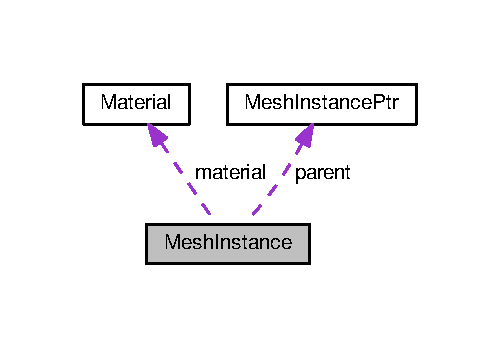
\includegraphics[width=240pt]{class_mesh_instance__coll__graph}
\end{center}
\end{figure}
\subsection*{Public Member Functions}
\begin{DoxyCompactItemize}
\item 
\hyperlink{class_mesh_instance_a0433e083188a2bef4f193032bba3b21f}{Mesh\+Instance} (\hyperlink{class_mesh_instance_ptr}{Mesh\+Instance\+Ptr} \hyperlink{class_mesh_instance_ad248a44f589cbeb5a8ec8748afebdcd8}{parent}, glm\+::mat4 \hyperlink{class_mesh_instance_a4ed7a3e07affd6862213ff054caa1b30}{instance\+Mat}, \hyperlink{struct_material}{Material} \hyperlink{class_mesh_instance_adba237cd83810b3afa89f1b911997e17}{material})
\item 
\hyperlink{class_mesh_instance_a9489df3dba59756832ad3789d6ae6b19}{Mesh\+Instance} (\hyperlink{class_mesh_instance_ptr}{Mesh\+Instance\+Ptr} \hyperlink{class_mesh_instance_ad248a44f589cbeb5a8ec8748afebdcd8}{parent})
\item 
\hyperlink{class_mesh_instance_ptr}{Mesh\+Instance\+Ptr} \hyperlink{class_mesh_instance_a0fa7328a13f39ddecefbd791bb8a60d4}{translate} (glm\+::vec3 t)
\item 
\hyperlink{class_mesh_instance_ptr}{Mesh\+Instance\+Ptr} \hyperlink{class_mesh_instance_a2f326744ece4345c59cfa56823693440}{scale} (glm\+::vec3 s)
\item 
\hyperlink{class_mesh_instance_ptr}{Mesh\+Instance\+Ptr} \hyperlink{class_mesh_instance_a63c843a137a99cdb24a06c8d3951c8a5}{rotate} (float angle, glm\+::vec3 axis)
\item 
\hyperlink{class_mesh_instance_ptr}{Mesh\+Instance\+Ptr} \hyperlink{class_mesh_instance_a76c43b6e1efab3b95027fdf7fc17a97d}{apply\+Matrix} (glm\+::mat4 transform)
\item 
\hyperlink{class_mesh_instance_a130ba9587f476a8897f704eaed1ebded}{Mesh\+Instance} (unsigned int \hyperlink{class_mesh_instance_a969bc28f038cda422be9efe24c308b58}{model\+Index}, unsigned int \hyperlink{class_mesh_instance_aec954bfbb05fd9d2e4da020ca61b8c35}{mesh\+Id}, \hyperlink{struct_material}{Material} \hyperlink{class_mesh_instance_adba237cd83810b3afa89f1b911997e17}{material})
\item 
\hyperlink{class_mesh_instance}{Mesh\+Instance} $\ast$ \hyperlink{class_mesh_instance_afdb729a6fbb69dcbf75dd926344cecac}{copy} ()
\item 
\hyperlink{class_mesh_instance}{Mesh\+Instance} $\ast$ \hyperlink{class_mesh_instance_a61840ca9d6395ea62a2ea230306e0ed6}{translate} (glm\+::vec3 t)
\item 
\hyperlink{class_mesh_instance}{Mesh\+Instance} $\ast$ \hyperlink{class_mesh_instance_a4968f7898f2eaa54921b08313fc79d31}{scale} (glm\+::vec3 s)
\item 
\hyperlink{class_mesh_instance}{Mesh\+Instance} $\ast$ \hyperlink{class_mesh_instance_a26db238575ab880fdc81d128051e6011}{rotate} (float angle, glm\+::vec3 axis)
\end{DoxyCompactItemize}
\subsection*{Public Attributes}
\begin{DoxyCompactItemize}
\item 
glm\+::mat4 \hyperlink{class_mesh_instance_a4ed7a3e07affd6862213ff054caa1b30}{instance\+Mat} = glm\+::mat4(1)
\item 
\hyperlink{struct_material}{Material} \hyperlink{class_mesh_instance_adba237cd83810b3afa89f1b911997e17}{material}
\item 
unsigned int \hyperlink{class_mesh_instance_a969bc28f038cda422be9efe24c308b58}{model\+Index}
\item 
unsigned int \hyperlink{class_mesh_instance_aec954bfbb05fd9d2e4da020ca61b8c35}{mesh\+Id}
\item 
unsigned int \hyperlink{class_mesh_instance_ad3ce9b979b94b94c79d082009f2d62c7}{instance\+Id}
\end{DoxyCompactItemize}
\subsection*{Static Public Attributes}
\begin{DoxyCompactItemize}
\item 
static unsigned int \hyperlink{class_mesh_instance_abded40a314dd0d8954d22bd24cdb6de8}{id\+Counter}
\end{DoxyCompactItemize}
\subsection*{Protected Attributes}
\begin{DoxyCompactItemize}
\item 
\hyperlink{class_mesh_instance_ptr}{Mesh\+Instance\+Ptr} \hyperlink{class_mesh_instance_ad248a44f589cbeb5a8ec8748afebdcd8}{parent}
\end{DoxyCompactItemize}


\subsection{Constructor \& Destructor Documentation}
\index{Mesh\+Instance@{Mesh\+Instance}!Mesh\+Instance@{Mesh\+Instance}}
\index{Mesh\+Instance@{Mesh\+Instance}!Mesh\+Instance@{Mesh\+Instance}}
\subsubsection[{\texorpdfstring{Mesh\+Instance(\+Mesh\+Instance\+Ptr parent, glm\+::mat4 instance\+Mat, Material material)}{MeshInstance(MeshInstancePtr parent, glm::mat4 instanceMat, Material material)}}]{\setlength{\rightskip}{0pt plus 5cm}Mesh\+Instance\+::\+Mesh\+Instance (
\begin{DoxyParamCaption}
\item[{{\bf Mesh\+Instance\+Ptr}}]{parent, }
\item[{glm\+::mat4}]{instance\+Mat, }
\item[{{\bf Material}}]{material}
\end{DoxyParamCaption}
)\hspace{0.3cm}{\ttfamily [inline]}}\hypertarget{class_mesh_instance_a0433e083188a2bef4f193032bba3b21f}{}\label{class_mesh_instance_a0433e083188a2bef4f193032bba3b21f}
\index{Mesh\+Instance@{Mesh\+Instance}!Mesh\+Instance@{Mesh\+Instance}}
\index{Mesh\+Instance@{Mesh\+Instance}!Mesh\+Instance@{Mesh\+Instance}}
\subsubsection[{\texorpdfstring{Mesh\+Instance(\+Mesh\+Instance\+Ptr parent)}{MeshInstance(MeshInstancePtr parent)}}]{\setlength{\rightskip}{0pt plus 5cm}Mesh\+Instance\+::\+Mesh\+Instance (
\begin{DoxyParamCaption}
\item[{{\bf Mesh\+Instance\+Ptr}}]{parent}
\end{DoxyParamCaption}
)\hspace{0.3cm}{\ttfamily [inline]}}\hypertarget{class_mesh_instance_a9489df3dba59756832ad3789d6ae6b19}{}\label{class_mesh_instance_a9489df3dba59756832ad3789d6ae6b19}
\index{Mesh\+Instance@{Mesh\+Instance}!Mesh\+Instance@{Mesh\+Instance}}
\index{Mesh\+Instance@{Mesh\+Instance}!Mesh\+Instance@{Mesh\+Instance}}
\subsubsection[{\texorpdfstring{Mesh\+Instance(unsigned int model\+Index, unsigned int mesh\+Id, Material material)}{MeshInstance(unsigned int modelIndex, unsigned int meshId, Material material)}}]{\setlength{\rightskip}{0pt plus 5cm}Mesh\+Instance\+::\+Mesh\+Instance (
\begin{DoxyParamCaption}
\item[{unsigned int}]{model\+Index, }
\item[{unsigned int}]{mesh\+Id, }
\item[{{\bf Material}}]{material}
\end{DoxyParamCaption}
)}\hypertarget{class_mesh_instance_a130ba9587f476a8897f704eaed1ebded}{}\label{class_mesh_instance_a130ba9587f476a8897f704eaed1ebded}


\subsection{Member Function Documentation}
\index{Mesh\+Instance@{Mesh\+Instance}!apply\+Matrix@{apply\+Matrix}}
\index{apply\+Matrix@{apply\+Matrix}!Mesh\+Instance@{Mesh\+Instance}}
\subsubsection[{\texorpdfstring{apply\+Matrix(glm\+::mat4 transform)}{applyMatrix(glm::mat4 transform)}}]{\setlength{\rightskip}{0pt plus 5cm}{\bf Mesh\+Instance\+Ptr} Mesh\+Instance\+::apply\+Matrix (
\begin{DoxyParamCaption}
\item[{glm\+::mat4}]{transform}
\end{DoxyParamCaption}
)\hspace{0.3cm}{\ttfamily [inline]}}\hypertarget{class_mesh_instance_a76c43b6e1efab3b95027fdf7fc17a97d}{}\label{class_mesh_instance_a76c43b6e1efab3b95027fdf7fc17a97d}
\index{Mesh\+Instance@{Mesh\+Instance}!copy@{copy}}
\index{copy@{copy}!Mesh\+Instance@{Mesh\+Instance}}
\subsubsection[{\texorpdfstring{copy()}{copy()}}]{\setlength{\rightskip}{0pt plus 5cm}{\bf Mesh\+Instance}$\ast$ Mesh\+Instance\+::copy (
\begin{DoxyParamCaption}
{}
\end{DoxyParamCaption}
)}\hypertarget{class_mesh_instance_afdb729a6fbb69dcbf75dd926344cecac}{}\label{class_mesh_instance_afdb729a6fbb69dcbf75dd926344cecac}
\index{Mesh\+Instance@{Mesh\+Instance}!rotate@{rotate}}
\index{rotate@{rotate}!Mesh\+Instance@{Mesh\+Instance}}
\subsubsection[{\texorpdfstring{rotate(float angle, glm\+::vec3 axis)}{rotate(float angle, glm::vec3 axis)}}]{\setlength{\rightskip}{0pt plus 5cm}{\bf Mesh\+Instance}$\ast$ Mesh\+Instance\+::rotate (
\begin{DoxyParamCaption}
\item[{float}]{angle, }
\item[{glm\+::vec3}]{axis}
\end{DoxyParamCaption}
)}\hypertarget{class_mesh_instance_a26db238575ab880fdc81d128051e6011}{}\label{class_mesh_instance_a26db238575ab880fdc81d128051e6011}
\index{Mesh\+Instance@{Mesh\+Instance}!rotate@{rotate}}
\index{rotate@{rotate}!Mesh\+Instance@{Mesh\+Instance}}
\subsubsection[{\texorpdfstring{rotate(float angle, glm\+::vec3 axis)}{rotate(float angle, glm::vec3 axis)}}]{\setlength{\rightskip}{0pt plus 5cm}{\bf Mesh\+Instance\+Ptr} Mesh\+Instance\+::rotate (
\begin{DoxyParamCaption}
\item[{float}]{angle, }
\item[{glm\+::vec3}]{axis}
\end{DoxyParamCaption}
)\hspace{0.3cm}{\ttfamily [inline]}}\hypertarget{class_mesh_instance_a63c843a137a99cdb24a06c8d3951c8a5}{}\label{class_mesh_instance_a63c843a137a99cdb24a06c8d3951c8a5}
\index{Mesh\+Instance@{Mesh\+Instance}!scale@{scale}}
\index{scale@{scale}!Mesh\+Instance@{Mesh\+Instance}}
\subsubsection[{\texorpdfstring{scale(glm\+::vec3 s)}{scale(glm::vec3 s)}}]{\setlength{\rightskip}{0pt plus 5cm}{\bf Mesh\+Instance}$\ast$ Mesh\+Instance\+::scale (
\begin{DoxyParamCaption}
\item[{glm\+::vec3}]{s}
\end{DoxyParamCaption}
)}\hypertarget{class_mesh_instance_a4968f7898f2eaa54921b08313fc79d31}{}\label{class_mesh_instance_a4968f7898f2eaa54921b08313fc79d31}
\index{Mesh\+Instance@{Mesh\+Instance}!scale@{scale}}
\index{scale@{scale}!Mesh\+Instance@{Mesh\+Instance}}
\subsubsection[{\texorpdfstring{scale(glm\+::vec3 s)}{scale(glm::vec3 s)}}]{\setlength{\rightskip}{0pt plus 5cm}{\bf Mesh\+Instance\+Ptr} Mesh\+Instance\+::scale (
\begin{DoxyParamCaption}
\item[{glm\+::vec3}]{s}
\end{DoxyParamCaption}
)\hspace{0.3cm}{\ttfamily [inline]}}\hypertarget{class_mesh_instance_a2f326744ece4345c59cfa56823693440}{}\label{class_mesh_instance_a2f326744ece4345c59cfa56823693440}
\index{Mesh\+Instance@{Mesh\+Instance}!translate@{translate}}
\index{translate@{translate}!Mesh\+Instance@{Mesh\+Instance}}
\subsubsection[{\texorpdfstring{translate(glm\+::vec3 t)}{translate(glm::vec3 t)}}]{\setlength{\rightskip}{0pt plus 5cm}{\bf Mesh\+Instance}$\ast$ Mesh\+Instance\+::translate (
\begin{DoxyParamCaption}
\item[{glm\+::vec3}]{t}
\end{DoxyParamCaption}
)}\hypertarget{class_mesh_instance_a61840ca9d6395ea62a2ea230306e0ed6}{}\label{class_mesh_instance_a61840ca9d6395ea62a2ea230306e0ed6}
\index{Mesh\+Instance@{Mesh\+Instance}!translate@{translate}}
\index{translate@{translate}!Mesh\+Instance@{Mesh\+Instance}}
\subsubsection[{\texorpdfstring{translate(glm\+::vec3 t)}{translate(glm::vec3 t)}}]{\setlength{\rightskip}{0pt plus 5cm}{\bf Mesh\+Instance\+Ptr} Mesh\+Instance\+::translate (
\begin{DoxyParamCaption}
\item[{glm\+::vec3}]{t}
\end{DoxyParamCaption}
)\hspace{0.3cm}{\ttfamily [inline]}}\hypertarget{class_mesh_instance_a0fa7328a13f39ddecefbd791bb8a60d4}{}\label{class_mesh_instance_a0fa7328a13f39ddecefbd791bb8a60d4}


\subsection{Member Data Documentation}
\index{Mesh\+Instance@{Mesh\+Instance}!id\+Counter@{id\+Counter}}
\index{id\+Counter@{id\+Counter}!Mesh\+Instance@{Mesh\+Instance}}
\subsubsection[{\texorpdfstring{id\+Counter}{idCounter}}]{\setlength{\rightskip}{0pt plus 5cm}unsigned int Mesh\+Instance\+::id\+Counter\hspace{0.3cm}{\ttfamily [static]}}\hypertarget{class_mesh_instance_abded40a314dd0d8954d22bd24cdb6de8}{}\label{class_mesh_instance_abded40a314dd0d8954d22bd24cdb6de8}
\index{Mesh\+Instance@{Mesh\+Instance}!instance\+Id@{instance\+Id}}
\index{instance\+Id@{instance\+Id}!Mesh\+Instance@{Mesh\+Instance}}
\subsubsection[{\texorpdfstring{instance\+Id}{instanceId}}]{\setlength{\rightskip}{0pt plus 5cm}unsigned int Mesh\+Instance\+::instance\+Id}\hypertarget{class_mesh_instance_ad3ce9b979b94b94c79d082009f2d62c7}{}\label{class_mesh_instance_ad3ce9b979b94b94c79d082009f2d62c7}
\index{Mesh\+Instance@{Mesh\+Instance}!instance\+Mat@{instance\+Mat}}
\index{instance\+Mat@{instance\+Mat}!Mesh\+Instance@{Mesh\+Instance}}
\subsubsection[{\texorpdfstring{instance\+Mat}{instanceMat}}]{\setlength{\rightskip}{0pt plus 5cm}glm\+::mat4 Mesh\+Instance\+::instance\+Mat = glm\+::mat4(1)}\hypertarget{class_mesh_instance_a4ed7a3e07affd6862213ff054caa1b30}{}\label{class_mesh_instance_a4ed7a3e07affd6862213ff054caa1b30}
\index{Mesh\+Instance@{Mesh\+Instance}!material@{material}}
\index{material@{material}!Mesh\+Instance@{Mesh\+Instance}}
\subsubsection[{\texorpdfstring{material}{material}}]{\setlength{\rightskip}{0pt plus 5cm}{\bf Material} Mesh\+Instance\+::material}\hypertarget{class_mesh_instance_adba237cd83810b3afa89f1b911997e17}{}\label{class_mesh_instance_adba237cd83810b3afa89f1b911997e17}
\index{Mesh\+Instance@{Mesh\+Instance}!mesh\+Id@{mesh\+Id}}
\index{mesh\+Id@{mesh\+Id}!Mesh\+Instance@{Mesh\+Instance}}
\subsubsection[{\texorpdfstring{mesh\+Id}{meshId}}]{\setlength{\rightskip}{0pt plus 5cm}unsigned int Mesh\+Instance\+::mesh\+Id}\hypertarget{class_mesh_instance_aec954bfbb05fd9d2e4da020ca61b8c35}{}\label{class_mesh_instance_aec954bfbb05fd9d2e4da020ca61b8c35}
\index{Mesh\+Instance@{Mesh\+Instance}!model\+Index@{model\+Index}}
\index{model\+Index@{model\+Index}!Mesh\+Instance@{Mesh\+Instance}}
\subsubsection[{\texorpdfstring{model\+Index}{modelIndex}}]{\setlength{\rightskip}{0pt plus 5cm}unsigned int Mesh\+Instance\+::model\+Index}\hypertarget{class_mesh_instance_a969bc28f038cda422be9efe24c308b58}{}\label{class_mesh_instance_a969bc28f038cda422be9efe24c308b58}
\index{Mesh\+Instance@{Mesh\+Instance}!parent@{parent}}
\index{parent@{parent}!Mesh\+Instance@{Mesh\+Instance}}
\subsubsection[{\texorpdfstring{parent}{parent}}]{\setlength{\rightskip}{0pt plus 5cm}{\bf Mesh\+Instance\+Ptr} Mesh\+Instance\+::parent\hspace{0.3cm}{\ttfamily [protected]}}\hypertarget{class_mesh_instance_ad248a44f589cbeb5a8ec8748afebdcd8}{}\label{class_mesh_instance_ad248a44f589cbeb5a8ec8748afebdcd8}


The documentation for this class was generated from the following files\+:\begin{DoxyCompactItemize}
\item 
src/\hyperlink{_mesh_8h}{Mesh.\+h}\item 
src/\hyperlink{_mesh_instance_8h}{Mesh\+Instance.\+h}\end{DoxyCompactItemize}

\hypertarget{class_mesh_instance_ptr}{}\section{Mesh\+Instance\+Ptr Class Reference}
\label{class_mesh_instance_ptr}\index{Mesh\+Instance\+Ptr@{Mesh\+Instance\+Ptr}}


{\ttfamily \#include $<$Mesh.\+h$>$}

\subsection*{Public Types}
\begin{DoxyCompactItemize}
\item 
typedef vector$<$ \hyperlink{class_mesh_instance}{Mesh\+Instance} $>$\+::\hyperlink{class_mesh_instance_ptr_adec11b2e0c0dd52620a5672406a2ad4f}{size\+\_\+type} \hyperlink{class_mesh_instance_ptr_adec11b2e0c0dd52620a5672406a2ad4f}{size\+\_\+type}
\end{DoxyCompactItemize}
\subsection*{Public Member Functions}
\begin{DoxyCompactItemize}
\item 
\hyperlink{class_mesh_instance_ptr_ac1d5253802ac00867f05e966d9837946}{Mesh\+Instance\+Ptr} ()
\item 
\hyperlink{class_mesh_instance_ptr_aec9e641cbf2233a9adcc704d368fd6c9}{Mesh\+Instance\+Ptr} (vector$<$ \hyperlink{class_mesh_instance}{Mesh\+Instance} $>$ $\ast$\hyperlink{class_mesh_instance_ptr_ae87840735de9302d2011731219da5fd4}{container}, \hyperlink{class_mesh_instance_ptr_adec11b2e0c0dd52620a5672406a2ad4f}{size\+\_\+type} \hyperlink{class_mesh_instance_ptr_ad99534feeaecaafcf4d8329723de2ffd}{offset})
\item 
\hyperlink{class_mesh_instance}{Mesh\+Instance} \hyperlink{class_mesh_instance_ptr_a143f878734446121cb88b56627d4829b}{operator$\ast$} ()
\item 
\hyperlink{class_mesh_instance}{Mesh\+Instance} $\ast$ \hyperlink{class_mesh_instance_ptr_acb4b080f0cfa0e29bd27aa0e8f984a29}{operator-\/$>$} ()
\end{DoxyCompactItemize}
\subsection*{Protected Attributes}
\begin{DoxyCompactItemize}
\item 
bool \hyperlink{class_mesh_instance_ptr_a64b684e33c846dbcdff7b53188d41238}{is\+Null}
\item 
vector$<$ \hyperlink{class_mesh_instance}{Mesh\+Instance} $>$ $\ast$ \hyperlink{class_mesh_instance_ptr_ae87840735de9302d2011731219da5fd4}{container}
\item 
\hyperlink{class_mesh_instance_ptr_adec11b2e0c0dd52620a5672406a2ad4f}{size\+\_\+type} \hyperlink{class_mesh_instance_ptr_ad99534feeaecaafcf4d8329723de2ffd}{offset}
\end{DoxyCompactItemize}


\subsection{Member Typedef Documentation}
\index{Mesh\+Instance\+Ptr@{Mesh\+Instance\+Ptr}!size\+\_\+type@{size\+\_\+type}}
\index{size\+\_\+type@{size\+\_\+type}!Mesh\+Instance\+Ptr@{Mesh\+Instance\+Ptr}}
\subsubsection[{\texorpdfstring{size\+\_\+type}{size_type}}]{\setlength{\rightskip}{0pt plus 5cm}typedef vector$<${\bf Mesh\+Instance}$>$\+::{\bf size\+\_\+type} {\bf Mesh\+Instance\+Ptr\+::size\+\_\+type}}\hypertarget{class_mesh_instance_ptr_adec11b2e0c0dd52620a5672406a2ad4f}{}\label{class_mesh_instance_ptr_adec11b2e0c0dd52620a5672406a2ad4f}


\subsection{Constructor \& Destructor Documentation}
\index{Mesh\+Instance\+Ptr@{Mesh\+Instance\+Ptr}!Mesh\+Instance\+Ptr@{Mesh\+Instance\+Ptr}}
\index{Mesh\+Instance\+Ptr@{Mesh\+Instance\+Ptr}!Mesh\+Instance\+Ptr@{Mesh\+Instance\+Ptr}}
\subsubsection[{\texorpdfstring{Mesh\+Instance\+Ptr()}{MeshInstancePtr()}}]{\setlength{\rightskip}{0pt plus 5cm}Mesh\+Instance\+Ptr\+::\+Mesh\+Instance\+Ptr (
\begin{DoxyParamCaption}
{}
\end{DoxyParamCaption}
)\hspace{0.3cm}{\ttfamily [inline]}}\hypertarget{class_mesh_instance_ptr_ac1d5253802ac00867f05e966d9837946}{}\label{class_mesh_instance_ptr_ac1d5253802ac00867f05e966d9837946}
\index{Mesh\+Instance\+Ptr@{Mesh\+Instance\+Ptr}!Mesh\+Instance\+Ptr@{Mesh\+Instance\+Ptr}}
\index{Mesh\+Instance\+Ptr@{Mesh\+Instance\+Ptr}!Mesh\+Instance\+Ptr@{Mesh\+Instance\+Ptr}}
\subsubsection[{\texorpdfstring{Mesh\+Instance\+Ptr(vector$<$ Mesh\+Instance $>$ $\ast$container, size\+\_\+type offset)}{MeshInstancePtr(vector< MeshInstance > *container, size_type offset)}}]{\setlength{\rightskip}{0pt plus 5cm}Mesh\+Instance\+Ptr\+::\+Mesh\+Instance\+Ptr (
\begin{DoxyParamCaption}
\item[{vector$<$ {\bf Mesh\+Instance} $>$ $\ast$}]{container, }
\item[{{\bf size\+\_\+type}}]{offset}
\end{DoxyParamCaption}
)\hspace{0.3cm}{\ttfamily [inline]}}\hypertarget{class_mesh_instance_ptr_aec9e641cbf2233a9adcc704d368fd6c9}{}\label{class_mesh_instance_ptr_aec9e641cbf2233a9adcc704d368fd6c9}


\subsection{Member Function Documentation}
\index{Mesh\+Instance\+Ptr@{Mesh\+Instance\+Ptr}!operator$\ast$@{operator$\ast$}}
\index{operator$\ast$@{operator$\ast$}!Mesh\+Instance\+Ptr@{Mesh\+Instance\+Ptr}}
\subsubsection[{\texorpdfstring{operator$\ast$()}{operator*()}}]{\setlength{\rightskip}{0pt plus 5cm}{\bf Mesh\+Instance} Mesh\+Instance\+Ptr\+::operator$\ast$ (
\begin{DoxyParamCaption}
{}
\end{DoxyParamCaption}
)}\hypertarget{class_mesh_instance_ptr_a143f878734446121cb88b56627d4829b}{}\label{class_mesh_instance_ptr_a143f878734446121cb88b56627d4829b}
\index{Mesh\+Instance\+Ptr@{Mesh\+Instance\+Ptr}!operator-\/$>$@{operator-\/$>$}}
\index{operator-\/$>$@{operator-\/$>$}!Mesh\+Instance\+Ptr@{Mesh\+Instance\+Ptr}}
\subsubsection[{\texorpdfstring{operator-\/$>$()}{operator->()}}]{\setlength{\rightskip}{0pt plus 5cm}{\bf Mesh\+Instance} $\ast$ Mesh\+Instance\+Ptr\+::operator-\/$>$ (
\begin{DoxyParamCaption}
{}
\end{DoxyParamCaption}
)}\hypertarget{class_mesh_instance_ptr_acb4b080f0cfa0e29bd27aa0e8f984a29}{}\label{class_mesh_instance_ptr_acb4b080f0cfa0e29bd27aa0e8f984a29}


\subsection{Member Data Documentation}
\index{Mesh\+Instance\+Ptr@{Mesh\+Instance\+Ptr}!container@{container}}
\index{container@{container}!Mesh\+Instance\+Ptr@{Mesh\+Instance\+Ptr}}
\subsubsection[{\texorpdfstring{container}{container}}]{\setlength{\rightskip}{0pt plus 5cm}vector$<${\bf Mesh\+Instance}$>$$\ast$ Mesh\+Instance\+Ptr\+::container\hspace{0.3cm}{\ttfamily [protected]}}\hypertarget{class_mesh_instance_ptr_ae87840735de9302d2011731219da5fd4}{}\label{class_mesh_instance_ptr_ae87840735de9302d2011731219da5fd4}
\index{Mesh\+Instance\+Ptr@{Mesh\+Instance\+Ptr}!is\+Null@{is\+Null}}
\index{is\+Null@{is\+Null}!Mesh\+Instance\+Ptr@{Mesh\+Instance\+Ptr}}
\subsubsection[{\texorpdfstring{is\+Null}{isNull}}]{\setlength{\rightskip}{0pt plus 5cm}bool Mesh\+Instance\+Ptr\+::is\+Null\hspace{0.3cm}{\ttfamily [protected]}}\hypertarget{class_mesh_instance_ptr_a64b684e33c846dbcdff7b53188d41238}{}\label{class_mesh_instance_ptr_a64b684e33c846dbcdff7b53188d41238}
\index{Mesh\+Instance\+Ptr@{Mesh\+Instance\+Ptr}!offset@{offset}}
\index{offset@{offset}!Mesh\+Instance\+Ptr@{Mesh\+Instance\+Ptr}}
\subsubsection[{\texorpdfstring{offset}{offset}}]{\setlength{\rightskip}{0pt plus 5cm}{\bf size\+\_\+type} Mesh\+Instance\+Ptr\+::offset\hspace{0.3cm}{\ttfamily [protected]}}\hypertarget{class_mesh_instance_ptr_ad99534feeaecaafcf4d8329723de2ffd}{}\label{class_mesh_instance_ptr_ad99534feeaecaafcf4d8329723de2ffd}


The documentation for this class was generated from the following files\+:\begin{DoxyCompactItemize}
\item 
src/\hyperlink{_mesh_8h}{Mesh.\+h}\item 
src/\hyperlink{_mesh_8cpp}{Mesh.\+cpp}\end{DoxyCompactItemize}

\hypertarget{class_model}{}\section{Model Class Reference}
\label{class_model}\index{Model@{Model}}


{\ttfamily \#include $<$Model.\+h$>$}



Inheritance diagram for Model\+:\nopagebreak
\begin{figure}[H]
\begin{center}
\leavevmode
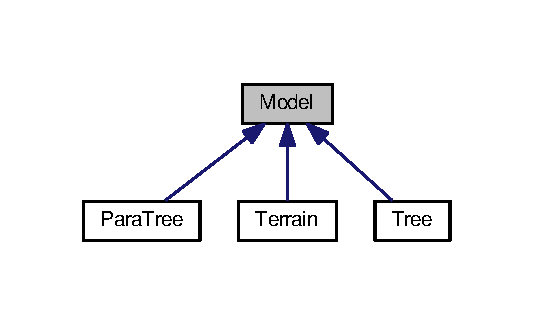
\includegraphics[width=256pt]{class_model__inherit__graph}
\end{center}
\end{figure}
\subsection*{Public Member Functions}
\begin{DoxyCompactItemize}
\item 
\hyperlink{class_model_ae3b375de5f6df4faf74a95d64748e048}{Model} ()
\item 
\hyperlink{class_mesh}{Mesh} $\ast$ \hyperlink{class_model_a0389a9deaec401c6050eddecfebd4eff}{new\+Mesh} (vector$<$ \hyperlink{struct_vertex}{Vertex} $>$ vertices, G\+Lenum draw\+Mode=G\+L\+\_\+\+T\+R\+I\+A\+N\+G\+L\+ES)
\item 
\hyperlink{class_mesh}{Mesh} $\ast$ \hyperlink{class_model_a1616abd0e910e0e8a9e37fe23d143ed5}{new\+Mesh} (vector$<$ \hyperlink{struct_vertex}{Vertex} $>$ vertices, vector$<$ G\+Luint $>$ indices, G\+Lenum draw\+Mode=G\+L\+\_\+\+T\+R\+I\+A\+N\+G\+L\+ES)
\item 
\hyperlink{class_mesh}{Mesh} $\ast$ \hyperlink{class_model_a5a54b1ec74ea98423c205d3fee7c744f}{new\+Mesh} (string file\+Path)
\item 
void \hyperlink{class_model_a967023af0128ffc4bb8609332234daea}{translate} (glm\+::vec3 t)
\item 
void \hyperlink{class_model_ac1cc7957271031bba837ba93e7f581e2}{scale} (glm\+::vec3 s)
\item 
void \hyperlink{class_model_a427830f435c2eb86481808d09b9fbe2d}{rotate} (float angle, glm\+::vec3 axis)
\item 
void \hyperlink{class_model_a083354971a2e7e1f4ac3efac85362f85}{draw} (\hyperlink{class_shader}{Shader} shader)
\end{DoxyCompactItemize}
\subsection*{Protected Attributes}
\begin{DoxyCompactItemize}
\item 
glm\+::mat4 \hyperlink{class_model_ad822f014d9b52f776d888b282d1924df}{model\+Mat}
\item 
list$<$ \hyperlink{class_mesh}{Mesh} $>$ \hyperlink{class_model_a4b0be9742b35855d9444179ab26f616f}{meshes}
\end{DoxyCompactItemize}


\subsection{Constructor \& Destructor Documentation}
\index{Model@{Model}!Model@{Model}}
\index{Model@{Model}!Model@{Model}}
\subsubsection[{\texorpdfstring{Model()}{Model()}}]{\setlength{\rightskip}{0pt plus 5cm}Model\+::\+Model (
\begin{DoxyParamCaption}
{}
\end{DoxyParamCaption}
)}\hypertarget{class_model_ae3b375de5f6df4faf74a95d64748e048}{}\label{class_model_ae3b375de5f6df4faf74a95d64748e048}


\subsection{Member Function Documentation}
\index{Model@{Model}!draw@{draw}}
\index{draw@{draw}!Model@{Model}}
\subsubsection[{\texorpdfstring{draw(\+Shader shader)}{draw(Shader shader)}}]{\setlength{\rightskip}{0pt plus 5cm}void Model\+::draw (
\begin{DoxyParamCaption}
\item[{{\bf Shader}}]{shader}
\end{DoxyParamCaption}
)}\hypertarget{class_model_a083354971a2e7e1f4ac3efac85362f85}{}\label{class_model_a083354971a2e7e1f4ac3efac85362f85}
\index{Model@{Model}!new\+Mesh@{new\+Mesh}}
\index{new\+Mesh@{new\+Mesh}!Model@{Model}}
\subsubsection[{\texorpdfstring{new\+Mesh(vector$<$ Vertex $>$ vertices, G\+Lenum draw\+Mode=\+G\+L\+\_\+\+T\+R\+I\+A\+N\+G\+L\+E\+S)}{newMesh(vector< Vertex > vertices, GLenum drawMode=GL_TRIANGLES)}}]{\setlength{\rightskip}{0pt plus 5cm}{\bf Mesh}$\ast$ Model\+::new\+Mesh (
\begin{DoxyParamCaption}
\item[{vector$<$ {\bf Vertex} $>$}]{vertices, }
\item[{G\+Lenum}]{draw\+Mode = {\ttfamily GL\+\_\+TRIANGLES}}
\end{DoxyParamCaption}
)\hspace{0.3cm}{\ttfamily [inline]}}\hypertarget{class_model_a0389a9deaec401c6050eddecfebd4eff}{}\label{class_model_a0389a9deaec401c6050eddecfebd4eff}
\index{Model@{Model}!new\+Mesh@{new\+Mesh}}
\index{new\+Mesh@{new\+Mesh}!Model@{Model}}
\subsubsection[{\texorpdfstring{new\+Mesh(vector$<$ Vertex $>$ vertices, vector$<$ G\+Luint $>$ indices, G\+Lenum draw\+Mode=\+G\+L\+\_\+\+T\+R\+I\+A\+N\+G\+L\+E\+S)}{newMesh(vector< Vertex > vertices, vector< GLuint > indices, GLenum drawMode=GL_TRIANGLES)}}]{\setlength{\rightskip}{0pt plus 5cm}{\bf Mesh}$\ast$ Model\+::new\+Mesh (
\begin{DoxyParamCaption}
\item[{vector$<$ {\bf Vertex} $>$}]{vertices, }
\item[{vector$<$ G\+Luint $>$}]{indices, }
\item[{G\+Lenum}]{draw\+Mode = {\ttfamily GL\+\_\+TRIANGLES}}
\end{DoxyParamCaption}
)\hspace{0.3cm}{\ttfamily [inline]}}\hypertarget{class_model_a1616abd0e910e0e8a9e37fe23d143ed5}{}\label{class_model_a1616abd0e910e0e8a9e37fe23d143ed5}
\index{Model@{Model}!new\+Mesh@{new\+Mesh}}
\index{new\+Mesh@{new\+Mesh}!Model@{Model}}
\subsubsection[{\texorpdfstring{new\+Mesh(string file\+Path)}{newMesh(string filePath)}}]{\setlength{\rightskip}{0pt plus 5cm}{\bf Mesh}$\ast$ Model\+::new\+Mesh (
\begin{DoxyParamCaption}
\item[{string}]{file\+Path}
\end{DoxyParamCaption}
)\hspace{0.3cm}{\ttfamily [inline]}}\hypertarget{class_model_a5a54b1ec74ea98423c205d3fee7c744f}{}\label{class_model_a5a54b1ec74ea98423c205d3fee7c744f}
\index{Model@{Model}!rotate@{rotate}}
\index{rotate@{rotate}!Model@{Model}}
\subsubsection[{\texorpdfstring{rotate(float angle, glm\+::vec3 axis)}{rotate(float angle, glm::vec3 axis)}}]{\setlength{\rightskip}{0pt plus 5cm}void Model\+::rotate (
\begin{DoxyParamCaption}
\item[{float}]{angle, }
\item[{glm\+::vec3}]{axis}
\end{DoxyParamCaption}
)}\hypertarget{class_model_a427830f435c2eb86481808d09b9fbe2d}{}\label{class_model_a427830f435c2eb86481808d09b9fbe2d}
\index{Model@{Model}!scale@{scale}}
\index{scale@{scale}!Model@{Model}}
\subsubsection[{\texorpdfstring{scale(glm\+::vec3 s)}{scale(glm::vec3 s)}}]{\setlength{\rightskip}{0pt plus 5cm}void Model\+::scale (
\begin{DoxyParamCaption}
\item[{glm\+::vec3}]{s}
\end{DoxyParamCaption}
)}\hypertarget{class_model_ac1cc7957271031bba837ba93e7f581e2}{}\label{class_model_ac1cc7957271031bba837ba93e7f581e2}
\index{Model@{Model}!translate@{translate}}
\index{translate@{translate}!Model@{Model}}
\subsubsection[{\texorpdfstring{translate(glm\+::vec3 t)}{translate(glm::vec3 t)}}]{\setlength{\rightskip}{0pt plus 5cm}void Model\+::translate (
\begin{DoxyParamCaption}
\item[{glm\+::vec3}]{t}
\end{DoxyParamCaption}
)}\hypertarget{class_model_a967023af0128ffc4bb8609332234daea}{}\label{class_model_a967023af0128ffc4bb8609332234daea}


\subsection{Member Data Documentation}
\index{Model@{Model}!meshes@{meshes}}
\index{meshes@{meshes}!Model@{Model}}
\subsubsection[{\texorpdfstring{meshes}{meshes}}]{\setlength{\rightskip}{0pt plus 5cm}list$<${\bf Mesh}$>$ Model\+::meshes\hspace{0.3cm}{\ttfamily [protected]}}\hypertarget{class_model_a4b0be9742b35855d9444179ab26f616f}{}\label{class_model_a4b0be9742b35855d9444179ab26f616f}
\index{Model@{Model}!model\+Mat@{model\+Mat}}
\index{model\+Mat@{model\+Mat}!Model@{Model}}
\subsubsection[{\texorpdfstring{model\+Mat}{modelMat}}]{\setlength{\rightskip}{0pt plus 5cm}glm\+::mat4 Model\+::model\+Mat\hspace{0.3cm}{\ttfamily [protected]}}\hypertarget{class_model_ad822f014d9b52f776d888b282d1924df}{}\label{class_model_ad822f014d9b52f776d888b282d1924df}


The documentation for this class was generated from the following files\+:\begin{DoxyCompactItemize}
\item 
src/\hyperlink{_model_8h}{Model.\+h}\item 
src/\hyperlink{_model_8cpp}{Model.\+cpp}\end{DoxyCompactItemize}

\hypertarget{class_p_l_s_1_1_module}{}\section{P\+LS\+:\+:Module Class Reference}
\label{class_p_l_s_1_1_module}\index{P\+L\+S\+::\+Module@{P\+L\+S\+::\+Module}}


{\ttfamily \#include $<$P\+L\+S.\+h$>$}

\subsection*{Public Member Functions}
\begin{DoxyCompactItemize}
\item 
\hyperlink{class_p_l_s_1_1_module_a5ef6b2ef2146e3b676f9f09aa89eb7e6}{Module} (char \hyperlink{class_p_l_s_1_1_module_aff9d7d8f68f2574de9355e7c23bc55b2}{symbol})
\item 
\hyperlink{class_p_l_s_1_1_module_aff9927b4ecd59e3b47982a8b636e2e0b}{Module} (char \hyperlink{class_p_l_s_1_1_module_aff9d7d8f68f2574de9355e7c23bc55b2}{symbol}, \hyperlink{class_p_l_s_1_1_param}{Param} param)
\item 
\hyperlink{class_p_l_s_1_1_module_a1e45439bc8ad04b70894076db8400cf2}{Module} (char \hyperlink{class_p_l_s_1_1_module_aff9d7d8f68f2574de9355e7c23bc55b2}{symbol}, std\+::vector$<$ \hyperlink{class_p_l_s_1_1_param}{Param} $>$ \hyperlink{class_p_l_s_1_1_module_aacac04d530bfdfd688dfa0abe4654f4b}{params})
\item 
\hyperlink{class_p_l_s_1_1_module}{Module} \hyperlink{class_p_l_s_1_1_module_a6dea01da9bc678170fe0397462926a33}{eval} (std\+::vector$<$ float $>$ in\+Params)
\end{DoxyCompactItemize}
\subsection*{Public Attributes}
\begin{DoxyCompactItemize}
\item 
char \hyperlink{class_p_l_s_1_1_module_aff9d7d8f68f2574de9355e7c23bc55b2}{symbol}
\item 
std\+::vector$<$ \hyperlink{class_p_l_s_1_1_param}{Param} $>$ \hyperlink{class_p_l_s_1_1_module_aacac04d530bfdfd688dfa0abe4654f4b}{params}
\end{DoxyCompactItemize}


\subsection{Constructor \& Destructor Documentation}
\index{P\+L\+S\+::\+Module@{P\+L\+S\+::\+Module}!Module@{Module}}
\index{Module@{Module}!P\+L\+S\+::\+Module@{P\+L\+S\+::\+Module}}
\subsubsection[{\texorpdfstring{Module(char symbol)}{Module(char symbol)}}]{\setlength{\rightskip}{0pt plus 5cm}P\+L\+S\+::\+Module\+::\+Module (
\begin{DoxyParamCaption}
\item[{char}]{symbol}
\end{DoxyParamCaption}
)\hspace{0.3cm}{\ttfamily [inline]}}\hypertarget{class_p_l_s_1_1_module_a5ef6b2ef2146e3b676f9f09aa89eb7e6}{}\label{class_p_l_s_1_1_module_a5ef6b2ef2146e3b676f9f09aa89eb7e6}
\index{P\+L\+S\+::\+Module@{P\+L\+S\+::\+Module}!Module@{Module}}
\index{Module@{Module}!P\+L\+S\+::\+Module@{P\+L\+S\+::\+Module}}
\subsubsection[{\texorpdfstring{Module(char symbol, Param param)}{Module(char symbol, Param param)}}]{\setlength{\rightskip}{0pt plus 5cm}P\+L\+S\+::\+Module\+::\+Module (
\begin{DoxyParamCaption}
\item[{char}]{symbol, }
\item[{{\bf Param}}]{param}
\end{DoxyParamCaption}
)\hspace{0.3cm}{\ttfamily [inline]}}\hypertarget{class_p_l_s_1_1_module_aff9927b4ecd59e3b47982a8b636e2e0b}{}\label{class_p_l_s_1_1_module_aff9927b4ecd59e3b47982a8b636e2e0b}
\index{P\+L\+S\+::\+Module@{P\+L\+S\+::\+Module}!Module@{Module}}
\index{Module@{Module}!P\+L\+S\+::\+Module@{P\+L\+S\+::\+Module}}
\subsubsection[{\texorpdfstring{Module(char symbol, std\+::vector$<$ Param $>$ params)}{Module(char symbol, std::vector< Param > params)}}]{\setlength{\rightskip}{0pt plus 5cm}P\+L\+S\+::\+Module\+::\+Module (
\begin{DoxyParamCaption}
\item[{char}]{symbol, }
\item[{std\+::vector$<$ {\bf Param} $>$}]{params}
\end{DoxyParamCaption}
)\hspace{0.3cm}{\ttfamily [inline]}}\hypertarget{class_p_l_s_1_1_module_a1e45439bc8ad04b70894076db8400cf2}{}\label{class_p_l_s_1_1_module_a1e45439bc8ad04b70894076db8400cf2}


\subsection{Member Function Documentation}
\index{P\+L\+S\+::\+Module@{P\+L\+S\+::\+Module}!eval@{eval}}
\index{eval@{eval}!P\+L\+S\+::\+Module@{P\+L\+S\+::\+Module}}
\subsubsection[{\texorpdfstring{eval(std\+::vector$<$ float $>$ in\+Params)}{eval(std::vector< float > inParams)}}]{\setlength{\rightskip}{0pt plus 5cm}{\bf Module} P\+L\+S\+::\+Module\+::eval (
\begin{DoxyParamCaption}
\item[{std\+::vector$<$ float $>$}]{in\+Params}
\end{DoxyParamCaption}
)\hspace{0.3cm}{\ttfamily [inline]}}\hypertarget{class_p_l_s_1_1_module_a6dea01da9bc678170fe0397462926a33}{}\label{class_p_l_s_1_1_module_a6dea01da9bc678170fe0397462926a33}


\subsection{Member Data Documentation}
\index{P\+L\+S\+::\+Module@{P\+L\+S\+::\+Module}!params@{params}}
\index{params@{params}!P\+L\+S\+::\+Module@{P\+L\+S\+::\+Module}}
\subsubsection[{\texorpdfstring{params}{params}}]{\setlength{\rightskip}{0pt plus 5cm}std\+::vector$<${\bf Param}$>$ P\+L\+S\+::\+Module\+::params}\hypertarget{class_p_l_s_1_1_module_aacac04d530bfdfd688dfa0abe4654f4b}{}\label{class_p_l_s_1_1_module_aacac04d530bfdfd688dfa0abe4654f4b}
\index{P\+L\+S\+::\+Module@{P\+L\+S\+::\+Module}!symbol@{symbol}}
\index{symbol@{symbol}!P\+L\+S\+::\+Module@{P\+L\+S\+::\+Module}}
\subsubsection[{\texorpdfstring{symbol}{symbol}}]{\setlength{\rightskip}{0pt plus 5cm}char P\+L\+S\+::\+Module\+::symbol}\hypertarget{class_p_l_s_1_1_module_aff9d7d8f68f2574de9355e7c23bc55b2}{}\label{class_p_l_s_1_1_module_aff9d7d8f68f2574de9355e7c23bc55b2}


The documentation for this class was generated from the following file\+:\begin{DoxyCompactItemize}
\item 
src/\hyperlink{_p_l_s_8h}{P\+L\+S.\+h}\end{DoxyCompactItemize}

\hypertarget{class_p_l_s_1_1_param}{}\section{P\+LS\+:\+:Param Class Reference}
\label{class_p_l_s_1_1_param}\index{P\+L\+S\+::\+Param@{P\+L\+S\+::\+Param}}


{\ttfamily \#include $<$P\+L\+S.\+h$>$}

\subsection*{Public Member Functions}
\begin{DoxyCompactItemize}
\item 
\hyperlink{class_p_l_s_1_1_param_a4ed48beec57cd7ef95415c1572175036}{Param} (float val)
\item 
\hyperlink{class_p_l_s_1_1_param_a73d2429c8787a11efe2933a5b15dce70}{Param} (\hyperlink{class_p_l_s_a001f46380d29f9a3703cc78ee928b244}{ffloat\+\_\+t} func)
\item 
float \hyperlink{class_p_l_s_1_1_param_a7e26460656062bb1feac3dce68a794bc}{value} ()
\item 
float \hyperlink{class_p_l_s_1_1_param_a71f6c853f2b869897083a8e7559fb385}{value} (std\+::vector$<$ float $>$ in\+Params)
\end{DoxyCompactItemize}


\subsection{Constructor \& Destructor Documentation}
\index{P\+L\+S\+::\+Param@{P\+L\+S\+::\+Param}!Param@{Param}}
\index{Param@{Param}!P\+L\+S\+::\+Param@{P\+L\+S\+::\+Param}}
\subsubsection[{\texorpdfstring{Param(float val)}{Param(float val)}}]{\setlength{\rightskip}{0pt plus 5cm}P\+L\+S\+::\+Param\+::\+Param (
\begin{DoxyParamCaption}
\item[{float}]{val}
\end{DoxyParamCaption}
)\hspace{0.3cm}{\ttfamily [inline]}}\hypertarget{class_p_l_s_1_1_param_a4ed48beec57cd7ef95415c1572175036}{}\label{class_p_l_s_1_1_param_a4ed48beec57cd7ef95415c1572175036}
\index{P\+L\+S\+::\+Param@{P\+L\+S\+::\+Param}!Param@{Param}}
\index{Param@{Param}!P\+L\+S\+::\+Param@{P\+L\+S\+::\+Param}}
\subsubsection[{\texorpdfstring{Param(ffloat\+\_\+t func)}{Param(ffloat_t func)}}]{\setlength{\rightskip}{0pt plus 5cm}P\+L\+S\+::\+Param\+::\+Param (
\begin{DoxyParamCaption}
\item[{{\bf ffloat\+\_\+t}}]{func}
\end{DoxyParamCaption}
)\hspace{0.3cm}{\ttfamily [inline]}}\hypertarget{class_p_l_s_1_1_param_a73d2429c8787a11efe2933a5b15dce70}{}\label{class_p_l_s_1_1_param_a73d2429c8787a11efe2933a5b15dce70}


\subsection{Member Function Documentation}
\index{P\+L\+S\+::\+Param@{P\+L\+S\+::\+Param}!value@{value}}
\index{value@{value}!P\+L\+S\+::\+Param@{P\+L\+S\+::\+Param}}
\subsubsection[{\texorpdfstring{value()}{value()}}]{\setlength{\rightskip}{0pt plus 5cm}float P\+L\+S\+::\+Param\+::value (
\begin{DoxyParamCaption}
{}
\end{DoxyParamCaption}
)\hspace{0.3cm}{\ttfamily [inline]}}\hypertarget{class_p_l_s_1_1_param_a7e26460656062bb1feac3dce68a794bc}{}\label{class_p_l_s_1_1_param_a7e26460656062bb1feac3dce68a794bc}
\index{P\+L\+S\+::\+Param@{P\+L\+S\+::\+Param}!value@{value}}
\index{value@{value}!P\+L\+S\+::\+Param@{P\+L\+S\+::\+Param}}
\subsubsection[{\texorpdfstring{value(std\+::vector$<$ float $>$ in\+Params)}{value(std::vector< float > inParams)}}]{\setlength{\rightskip}{0pt plus 5cm}float P\+L\+S\+::\+Param\+::value (
\begin{DoxyParamCaption}
\item[{std\+::vector$<$ float $>$}]{in\+Params}
\end{DoxyParamCaption}
)\hspace{0.3cm}{\ttfamily [inline]}}\hypertarget{class_p_l_s_1_1_param_a71f6c853f2b869897083a8e7559fb385}{}\label{class_p_l_s_1_1_param_a71f6c853f2b869897083a8e7559fb385}


The documentation for this class was generated from the following file\+:\begin{DoxyCompactItemize}
\item 
src/\hyperlink{_p_l_s_8h}{P\+L\+S.\+h}\end{DoxyCompactItemize}

\hypertarget{class_para_tree}{}\section{Para\+Tree Class Reference}
\label{class_para_tree}\index{Para\+Tree@{Para\+Tree}}


{\ttfamily \#include $<$Para\+Tree.\+h$>$}



Inheritance diagram for Para\+Tree\+:\nopagebreak
\begin{figure}[H]
\begin{center}
\leavevmode
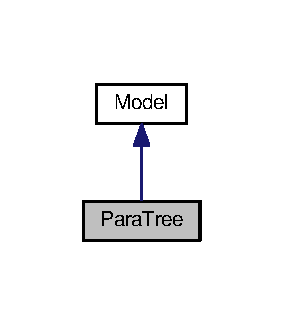
\includegraphics[width=136pt]{class_para_tree__inherit__graph}
\end{center}
\end{figure}


Collaboration diagram for Para\+Tree\+:\nopagebreak
\begin{figure}[H]
\begin{center}
\leavevmode
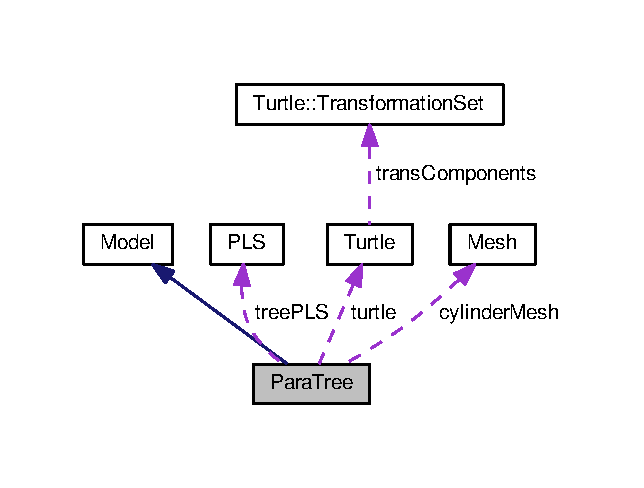
\includegraphics[width=309pt]{class_para_tree__coll__graph}
\end{center}
\end{figure}
\subsection*{Classes}
\begin{DoxyCompactItemize}
\item 
struct \hyperlink{struct_para_tree_1_1_actions}{Actions}
\item 
struct \hyperlink{struct_para_tree_1_1_presets}{Presets}
\item 
struct \hyperlink{struct_para_tree_1_1_tree_params}{Tree\+Params}
\end{DoxyCompactItemize}
\subsection*{Public Member Functions}
\begin{DoxyCompactItemize}
\item 
\hyperlink{class_para_tree_a061b04d1f938f69dd88c23ae98387f20}{Para\+Tree} (\hyperlink{struct_para_tree_1_1_tree_params}{Tree\+Params} tree\+Params=\hyperlink{struct_para_tree_1_1_presets_a140de0ee6d4a2eca71f2757e410e1aa0}{Presets\+::h})
\end{DoxyCompactItemize}
\subsection*{Protected Member Functions}
\begin{DoxyCompactItemize}
\item 
void \hyperlink{class_para_tree_a9619326b67874d3dc7792a88461a4c95}{generate} (unsigned int n)
\end{DoxyCompactItemize}
\subsection*{Protected Attributes}
\begin{DoxyCompactItemize}
\item 
\hyperlink{class_p_l_s}{P\+LS} \hyperlink{class_para_tree_a0de53b749e934865aa85cb20f2708e3f}{tree\+P\+LS}
\item 
\hyperlink{class_turtle}{Turtle} \hyperlink{class_para_tree_ab6f49307f128d77610ee0972a623abee}{turtle}
\item 
\hyperlink{class_mesh}{Mesh} $\ast$ \hyperlink{class_para_tree_a2efada45e3acee2f958be94b2ad6c5cd}{cylinder\+Mesh}
\end{DoxyCompactItemize}


\subsection{Constructor \& Destructor Documentation}
\index{Para\+Tree@{Para\+Tree}!Para\+Tree@{Para\+Tree}}
\index{Para\+Tree@{Para\+Tree}!Para\+Tree@{Para\+Tree}}
\subsubsection[{\texorpdfstring{Para\+Tree(\+Tree\+Params tree\+Params=\+Presets\+::h)}{ParaTree(TreeParams treeParams=Presets::h)}}]{\setlength{\rightskip}{0pt plus 5cm}Para\+Tree\+::\+Para\+Tree (
\begin{DoxyParamCaption}
\item[{{\bf Para\+Tree\+::\+Tree\+Params}}]{tree\+Params = {\ttfamily {\bf Presets\+::h}}}
\end{DoxyParamCaption}
)}\hypertarget{class_para_tree_a061b04d1f938f69dd88c23ae98387f20}{}\label{class_para_tree_a061b04d1f938f69dd88c23ae98387f20}


\subsection{Member Function Documentation}
\index{Para\+Tree@{Para\+Tree}!generate@{generate}}
\index{generate@{generate}!Para\+Tree@{Para\+Tree}}
\subsubsection[{\texorpdfstring{generate(unsigned int n)}{generate(unsigned int n)}}]{\setlength{\rightskip}{0pt plus 5cm}void Para\+Tree\+::generate (
\begin{DoxyParamCaption}
\item[{unsigned int}]{n}
\end{DoxyParamCaption}
)\hspace{0.3cm}{\ttfamily [protected]}}\hypertarget{class_para_tree_a9619326b67874d3dc7792a88461a4c95}{}\label{class_para_tree_a9619326b67874d3dc7792a88461a4c95}


\subsection{Member Data Documentation}
\index{Para\+Tree@{Para\+Tree}!cylinder\+Mesh@{cylinder\+Mesh}}
\index{cylinder\+Mesh@{cylinder\+Mesh}!Para\+Tree@{Para\+Tree}}
\subsubsection[{\texorpdfstring{cylinder\+Mesh}{cylinderMesh}}]{\setlength{\rightskip}{0pt plus 5cm}{\bf Mesh}$\ast$ Para\+Tree\+::cylinder\+Mesh\hspace{0.3cm}{\ttfamily [protected]}}\hypertarget{class_para_tree_a2efada45e3acee2f958be94b2ad6c5cd}{}\label{class_para_tree_a2efada45e3acee2f958be94b2ad6c5cd}
\index{Para\+Tree@{Para\+Tree}!tree\+P\+LS@{tree\+P\+LS}}
\index{tree\+P\+LS@{tree\+P\+LS}!Para\+Tree@{Para\+Tree}}
\subsubsection[{\texorpdfstring{tree\+P\+LS}{treePLS}}]{\setlength{\rightskip}{0pt plus 5cm}{\bf P\+LS} Para\+Tree\+::tree\+P\+LS\hspace{0.3cm}{\ttfamily [protected]}}\hypertarget{class_para_tree_a0de53b749e934865aa85cb20f2708e3f}{}\label{class_para_tree_a0de53b749e934865aa85cb20f2708e3f}
\index{Para\+Tree@{Para\+Tree}!turtle@{turtle}}
\index{turtle@{turtle}!Para\+Tree@{Para\+Tree}}
\subsubsection[{\texorpdfstring{turtle}{turtle}}]{\setlength{\rightskip}{0pt plus 5cm}{\bf Turtle} Para\+Tree\+::turtle\hspace{0.3cm}{\ttfamily [protected]}}\hypertarget{class_para_tree_ab6f49307f128d77610ee0972a623abee}{}\label{class_para_tree_ab6f49307f128d77610ee0972a623abee}


The documentation for this class was generated from the following files\+:\begin{DoxyCompactItemize}
\item 
src/\hyperlink{_para_tree_8h}{Para\+Tree.\+h}\item 
src/\hyperlink{_para_tree_8cpp}{Para\+Tree.\+cpp}\end{DoxyCompactItemize}

\hypertarget{class_p_l_s}{}\section{P\+LS Class Reference}
\label{class_p_l_s}\index{P\+LS@{P\+LS}}


{\ttfamily \#include $<$P\+L\+S.\+h$>$}

\subsection*{Classes}
\begin{DoxyCompactItemize}
\item 
class \hyperlink{class_p_l_s_1_1_module}{Module}
\item 
class \hyperlink{class_p_l_s_1_1_param}{Param}
\item 
class \hyperlink{class_p_l_s_1_1_production}{Production}
\end{DoxyCompactItemize}
\subsection*{Public Member Functions}
\begin{DoxyCompactItemize}
\item 
\hyperlink{class_p_l_s_a47c6fa2278f0d4a2f885484950211a5b}{P\+LS} (std\+::list$<$ \hyperlink{class_p_l_s_1_1_module}{Module} $>$ \hyperlink{class_p_l_s_a5de46c72cd9ef4006f7f1ed43ac028c1}{axiom}, std\+::unordered\+\_\+map$<$ char, \hyperlink{class_p_l_s_1_1_production}{Production} $>$ \hyperlink{class_p_l_s_a2bdf324e0d0ed4e1c3265d4029f83f0b}{productions}, std\+::unordered\+\_\+map$<$ char, \hyperlink{class_p_l_s_a2c9371dd235f3c41295d15c92ac9f33b}{fvoid\+\_\+t} $>$ \hyperlink{class_p_l_s_a5d7bf41cb569c111be4899bd7904a0da}{actions})
\item 
\hyperlink{class_p_l_s_a99f207f5849c3c1420da017e611d415a}{P\+LS} ()
\item 
void \hyperlink{class_p_l_s_a62156c4202b8cd20d4ba37306a57af87}{iterate} ()
\item 
void \hyperlink{class_p_l_s_ac87b2a52213e0e0a7fd0bcb969a68f8d}{iterate} (int n)
\item 
void \hyperlink{class_p_l_s_a72c26ad73b282abac9137978dcff21cb}{run} ()
\item 
std\+::list$<$ \hyperlink{class_p_l_s_1_1_module}{Module} $>$ \hyperlink{class_p_l_s_a26085d4c74f3ccddd6241cc9548e0d2a}{get\+Value} ()
\item 
unsigned int \hyperlink{class_p_l_s_aed7eff9d6f21452608d9f007f7ddaf26}{get\+Generation} ()
\end{DoxyCompactItemize}
\subsection*{Static Public Member Functions}
\begin{DoxyCompactItemize}
\item 
static float \hyperlink{class_p_l_s_a7a289ddec2b417d62e6137b798e1258f}{pass} (float a)
\item 
static float \hyperlink{class_p_l_s_a0437a3e9ba5cd3682573165ccc1fbf9c}{mult} (float a, float b)
\item 
static bool \hyperlink{class_p_l_s_ac8298e4b5940dae6c48e1dc042d4d8aa}{gteq} (float a, float b)
\end{DoxyCompactItemize}
\subsection*{Protected Types}
\begin{DoxyCompactItemize}
\item 
typedef std\+::function$<$ float(float, float, float, float, float)$>$ \hyperlink{class_p_l_s_a001f46380d29f9a3703cc78ee928b244}{ffloat\+\_\+t}
\item 
typedef std\+::function$<$ bool(float, float, float, float, float)$>$ \hyperlink{class_p_l_s_ae518559a64636a22c6e5f5eaa82cc420}{fbool\+\_\+t}
\item 
typedef std\+::function$<$ void(float, float, float, float, float)$>$ \hyperlink{class_p_l_s_a2c9371dd235f3c41295d15c92ac9f33b}{fvoid\+\_\+t}
\end{DoxyCompactItemize}
\subsection*{Protected Attributes}
\begin{DoxyCompactItemize}
\item 
std\+::list$<$ \hyperlink{class_p_l_s_1_1_module}{Module} $>$ \hyperlink{class_p_l_s_a5de46c72cd9ef4006f7f1ed43ac028c1}{axiom}
\item 
std\+::unordered\+\_\+map$<$ char, \hyperlink{class_p_l_s_1_1_production}{Production} $>$ \hyperlink{class_p_l_s_a2bdf324e0d0ed4e1c3265d4029f83f0b}{productions}
\item 
std\+::unordered\+\_\+map$<$ char, \hyperlink{class_p_l_s_a2c9371dd235f3c41295d15c92ac9f33b}{fvoid\+\_\+t} $>$ \hyperlink{class_p_l_s_a5d7bf41cb569c111be4899bd7904a0da}{actions}
\item 
std\+::list$<$ \hyperlink{class_p_l_s_1_1_module}{Module} $>$ \hyperlink{class_p_l_s_adf032e0f090c28370850ee026375f826}{value}
\item 
unsigned int \hyperlink{class_p_l_s_a056f4e66546bc58aaa68f68b6ac0e902}{generation}
\end{DoxyCompactItemize}


\subsection{Member Typedef Documentation}
\index{P\+LS@{P\+LS}!fbool\+\_\+t@{fbool\+\_\+t}}
\index{fbool\+\_\+t@{fbool\+\_\+t}!P\+LS@{P\+LS}}
\subsubsection[{\texorpdfstring{fbool\+\_\+t}{fbool_t}}]{\setlength{\rightskip}{0pt plus 5cm}typedef std\+::function$<$bool(float, float, float, float, float)$>$ {\bf P\+L\+S\+::fbool\+\_\+t}\hspace{0.3cm}{\ttfamily [protected]}}\hypertarget{class_p_l_s_ae518559a64636a22c6e5f5eaa82cc420}{}\label{class_p_l_s_ae518559a64636a22c6e5f5eaa82cc420}
\index{P\+LS@{P\+LS}!ffloat\+\_\+t@{ffloat\+\_\+t}}
\index{ffloat\+\_\+t@{ffloat\+\_\+t}!P\+LS@{P\+LS}}
\subsubsection[{\texorpdfstring{ffloat\+\_\+t}{ffloat_t}}]{\setlength{\rightskip}{0pt plus 5cm}typedef std\+::function$<$float(float, float, float, float, float)$>$ {\bf P\+L\+S\+::ffloat\+\_\+t}\hspace{0.3cm}{\ttfamily [protected]}}\hypertarget{class_p_l_s_a001f46380d29f9a3703cc78ee928b244}{}\label{class_p_l_s_a001f46380d29f9a3703cc78ee928b244}
\index{P\+LS@{P\+LS}!fvoid\+\_\+t@{fvoid\+\_\+t}}
\index{fvoid\+\_\+t@{fvoid\+\_\+t}!P\+LS@{P\+LS}}
\subsubsection[{\texorpdfstring{fvoid\+\_\+t}{fvoid_t}}]{\setlength{\rightskip}{0pt plus 5cm}typedef std\+::function$<$void(float, float, float, float, float)$>$ {\bf P\+L\+S\+::fvoid\+\_\+t}\hspace{0.3cm}{\ttfamily [protected]}}\hypertarget{class_p_l_s_a2c9371dd235f3c41295d15c92ac9f33b}{}\label{class_p_l_s_a2c9371dd235f3c41295d15c92ac9f33b}


\subsection{Constructor \& Destructor Documentation}
\index{P\+LS@{P\+LS}!P\+LS@{P\+LS}}
\index{P\+LS@{P\+LS}!P\+LS@{P\+LS}}
\subsubsection[{\texorpdfstring{P\+L\+S(std\+::list$<$ Module $>$ axiom, std\+::unordered\+\_\+map$<$ char, Production $>$ productions, std\+::unordered\+\_\+map$<$ char, fvoid\+\_\+t $>$ actions)}{PLS(std::list< Module > axiom, std::unordered_map< char, Production > productions, std::unordered_map< char, fvoid_t > actions)}}]{\setlength{\rightskip}{0pt plus 5cm}P\+L\+S\+::\+P\+LS (
\begin{DoxyParamCaption}
\item[{std\+::list$<$ {\bf Module} $>$}]{axiom, }
\item[{std\+::unordered\+\_\+map$<$ char, {\bf Production} $>$}]{productions, }
\item[{std\+::unordered\+\_\+map$<$ char, {\bf fvoid\+\_\+t} $>$}]{actions}
\end{DoxyParamCaption}
)\hspace{0.3cm}{\ttfamily [inline]}}\hypertarget{class_p_l_s_a47c6fa2278f0d4a2f885484950211a5b}{}\label{class_p_l_s_a47c6fa2278f0d4a2f885484950211a5b}
\index{P\+LS@{P\+LS}!P\+LS@{P\+LS}}
\index{P\+LS@{P\+LS}!P\+LS@{P\+LS}}
\subsubsection[{\texorpdfstring{P\+L\+S()}{PLS()}}]{\setlength{\rightskip}{0pt plus 5cm}P\+L\+S\+::\+P\+LS (
\begin{DoxyParamCaption}
{}
\end{DoxyParamCaption}
)\hspace{0.3cm}{\ttfamily [inline]}}\hypertarget{class_p_l_s_a99f207f5849c3c1420da017e611d415a}{}\label{class_p_l_s_a99f207f5849c3c1420da017e611d415a}


\subsection{Member Function Documentation}
\index{P\+LS@{P\+LS}!get\+Generation@{get\+Generation}}
\index{get\+Generation@{get\+Generation}!P\+LS@{P\+LS}}
\subsubsection[{\texorpdfstring{get\+Generation()}{getGeneration()}}]{\setlength{\rightskip}{0pt plus 5cm}unsigned int P\+L\+S\+::get\+Generation (
\begin{DoxyParamCaption}
{}
\end{DoxyParamCaption}
)\hspace{0.3cm}{\ttfamily [inline]}}\hypertarget{class_p_l_s_aed7eff9d6f21452608d9f007f7ddaf26}{}\label{class_p_l_s_aed7eff9d6f21452608d9f007f7ddaf26}
\index{P\+LS@{P\+LS}!get\+Value@{get\+Value}}
\index{get\+Value@{get\+Value}!P\+LS@{P\+LS}}
\subsubsection[{\texorpdfstring{get\+Value()}{getValue()}}]{\setlength{\rightskip}{0pt plus 5cm}std\+::list$<${\bf Module}$>$ P\+L\+S\+::get\+Value (
\begin{DoxyParamCaption}
{}
\end{DoxyParamCaption}
)\hspace{0.3cm}{\ttfamily [inline]}}\hypertarget{class_p_l_s_a26085d4c74f3ccddd6241cc9548e0d2a}{}\label{class_p_l_s_a26085d4c74f3ccddd6241cc9548e0d2a}
\index{P\+LS@{P\+LS}!gteq@{gteq}}
\index{gteq@{gteq}!P\+LS@{P\+LS}}
\subsubsection[{\texorpdfstring{gteq(float a, float b)}{gteq(float a, float b)}}]{\setlength{\rightskip}{0pt plus 5cm}static bool P\+L\+S\+::gteq (
\begin{DoxyParamCaption}
\item[{float}]{a, }
\item[{float}]{b}
\end{DoxyParamCaption}
)\hspace{0.3cm}{\ttfamily [inline]}, {\ttfamily [static]}}\hypertarget{class_p_l_s_ac8298e4b5940dae6c48e1dc042d4d8aa}{}\label{class_p_l_s_ac8298e4b5940dae6c48e1dc042d4d8aa}
\index{P\+LS@{P\+LS}!iterate@{iterate}}
\index{iterate@{iterate}!P\+LS@{P\+LS}}
\subsubsection[{\texorpdfstring{iterate()}{iterate()}}]{\setlength{\rightskip}{0pt plus 5cm}void P\+L\+S\+::iterate (
\begin{DoxyParamCaption}
{}
\end{DoxyParamCaption}
)\hspace{0.3cm}{\ttfamily [inline]}}\hypertarget{class_p_l_s_a62156c4202b8cd20d4ba37306a57af87}{}\label{class_p_l_s_a62156c4202b8cd20d4ba37306a57af87}
\index{P\+LS@{P\+LS}!iterate@{iterate}}
\index{iterate@{iterate}!P\+LS@{P\+LS}}
\subsubsection[{\texorpdfstring{iterate(int n)}{iterate(int n)}}]{\setlength{\rightskip}{0pt plus 5cm}void P\+L\+S\+::iterate (
\begin{DoxyParamCaption}
\item[{int}]{n}
\end{DoxyParamCaption}
)\hspace{0.3cm}{\ttfamily [inline]}}\hypertarget{class_p_l_s_ac87b2a52213e0e0a7fd0bcb969a68f8d}{}\label{class_p_l_s_ac87b2a52213e0e0a7fd0bcb969a68f8d}
\index{P\+LS@{P\+LS}!mult@{mult}}
\index{mult@{mult}!P\+LS@{P\+LS}}
\subsubsection[{\texorpdfstring{mult(float a, float b)}{mult(float a, float b)}}]{\setlength{\rightskip}{0pt plus 5cm}static float P\+L\+S\+::mult (
\begin{DoxyParamCaption}
\item[{float}]{a, }
\item[{float}]{b}
\end{DoxyParamCaption}
)\hspace{0.3cm}{\ttfamily [inline]}, {\ttfamily [static]}}\hypertarget{class_p_l_s_a0437a3e9ba5cd3682573165ccc1fbf9c}{}\label{class_p_l_s_a0437a3e9ba5cd3682573165ccc1fbf9c}
\index{P\+LS@{P\+LS}!pass@{pass}}
\index{pass@{pass}!P\+LS@{P\+LS}}
\subsubsection[{\texorpdfstring{pass(float a)}{pass(float a)}}]{\setlength{\rightskip}{0pt plus 5cm}static float P\+L\+S\+::pass (
\begin{DoxyParamCaption}
\item[{float}]{a}
\end{DoxyParamCaption}
)\hspace{0.3cm}{\ttfamily [inline]}, {\ttfamily [static]}}\hypertarget{class_p_l_s_a7a289ddec2b417d62e6137b798e1258f}{}\label{class_p_l_s_a7a289ddec2b417d62e6137b798e1258f}
\index{P\+LS@{P\+LS}!run@{run}}
\index{run@{run}!P\+LS@{P\+LS}}
\subsubsection[{\texorpdfstring{run()}{run()}}]{\setlength{\rightskip}{0pt plus 5cm}void P\+L\+S\+::run (
\begin{DoxyParamCaption}
{}
\end{DoxyParamCaption}
)\hspace{0.3cm}{\ttfamily [inline]}}\hypertarget{class_p_l_s_a72c26ad73b282abac9137978dcff21cb}{}\label{class_p_l_s_a72c26ad73b282abac9137978dcff21cb}


\subsection{Member Data Documentation}
\index{P\+LS@{P\+LS}!actions@{actions}}
\index{actions@{actions}!P\+LS@{P\+LS}}
\subsubsection[{\texorpdfstring{actions}{actions}}]{\setlength{\rightskip}{0pt plus 5cm}std\+::unordered\+\_\+map$<$char, {\bf fvoid\+\_\+t}$>$ P\+L\+S\+::actions\hspace{0.3cm}{\ttfamily [protected]}}\hypertarget{class_p_l_s_a5d7bf41cb569c111be4899bd7904a0da}{}\label{class_p_l_s_a5d7bf41cb569c111be4899bd7904a0da}
\index{P\+LS@{P\+LS}!axiom@{axiom}}
\index{axiom@{axiom}!P\+LS@{P\+LS}}
\subsubsection[{\texorpdfstring{axiom}{axiom}}]{\setlength{\rightskip}{0pt plus 5cm}std\+::list$<${\bf Module}$>$ P\+L\+S\+::axiom\hspace{0.3cm}{\ttfamily [protected]}}\hypertarget{class_p_l_s_a5de46c72cd9ef4006f7f1ed43ac028c1}{}\label{class_p_l_s_a5de46c72cd9ef4006f7f1ed43ac028c1}
\index{P\+LS@{P\+LS}!generation@{generation}}
\index{generation@{generation}!P\+LS@{P\+LS}}
\subsubsection[{\texorpdfstring{generation}{generation}}]{\setlength{\rightskip}{0pt plus 5cm}unsigned int P\+L\+S\+::generation\hspace{0.3cm}{\ttfamily [protected]}}\hypertarget{class_p_l_s_a056f4e66546bc58aaa68f68b6ac0e902}{}\label{class_p_l_s_a056f4e66546bc58aaa68f68b6ac0e902}
\index{P\+LS@{P\+LS}!productions@{productions}}
\index{productions@{productions}!P\+LS@{P\+LS}}
\subsubsection[{\texorpdfstring{productions}{productions}}]{\setlength{\rightskip}{0pt plus 5cm}std\+::unordered\+\_\+map$<$char, {\bf Production}$>$ P\+L\+S\+::productions\hspace{0.3cm}{\ttfamily [protected]}}\hypertarget{class_p_l_s_a2bdf324e0d0ed4e1c3265d4029f83f0b}{}\label{class_p_l_s_a2bdf324e0d0ed4e1c3265d4029f83f0b}
\index{P\+LS@{P\+LS}!value@{value}}
\index{value@{value}!P\+LS@{P\+LS}}
\subsubsection[{\texorpdfstring{value}{value}}]{\setlength{\rightskip}{0pt plus 5cm}std\+::list$<${\bf Module}$>$ P\+L\+S\+::value\hspace{0.3cm}{\ttfamily [protected]}}\hypertarget{class_p_l_s_adf032e0f090c28370850ee026375f826}{}\label{class_p_l_s_adf032e0f090c28370850ee026375f826}


The documentation for this class was generated from the following file\+:\begin{DoxyCompactItemize}
\item 
src/\hyperlink{_p_l_s_8h}{P\+L\+S.\+h}\end{DoxyCompactItemize}

\hypertarget{struct_para_tree_1_1_presets}{}\section{Para\+Tree\+:\+:Presets Struct Reference}
\label{struct_para_tree_1_1_presets}\index{Para\+Tree\+::\+Presets@{Para\+Tree\+::\+Presets}}


{\ttfamily \#include $<$Para\+Tree.\+h$>$}



Collaboration diagram for Para\+Tree\+:\+:Presets\+:\nopagebreak
\begin{figure}[H]
\begin{center}
\leavevmode
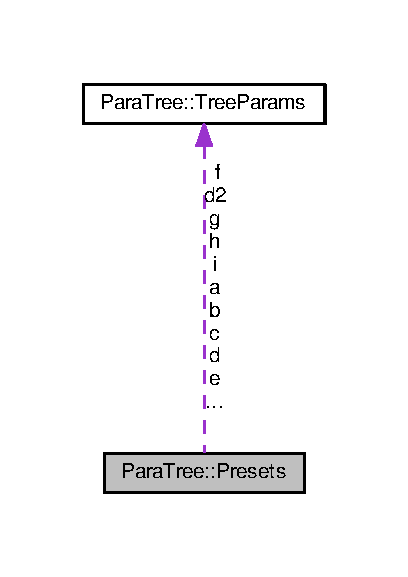
\includegraphics[width=196pt]{struct_para_tree_1_1_presets__coll__graph}
\end{center}
\end{figure}
\subsection*{Static Public Attributes}
\begin{DoxyCompactItemize}
\item 
static const \hyperlink{struct_para_tree_1_1_tree_params}{Tree\+Params} \hyperlink{struct_para_tree_1_1_presets_a91e10b4738fdd380fc676b38288cb81b}{a} = \{0.\+75, 0.\+77, 35, -\/35, 0, 0, 30, 0.\+50, 0.\+40, 0.\+0, 10\}
\item 
static const \hyperlink{struct_para_tree_1_1_tree_params}{Tree\+Params} \hyperlink{struct_para_tree_1_1_presets_a312f3c102ffcc4fcc6df99c28fc084d9}{b} = \{0.\+65, 0.\+71, 27, -\/68, 0, 0, 20, 0.\+53, 0.\+50, 1.\+7, 12\}
\item 
static const \hyperlink{struct_para_tree_1_1_tree_params}{Tree\+Params} \hyperlink{struct_para_tree_1_1_presets_a8ac6e067f498f41f6ce8d01f3c728be3}{c} = \{0.\+50, 0.\+85, 25, -\/15, 180, 0, 20, 0.\+45, 0.\+50, 0.\+5, 9\}
\item 
static const \hyperlink{struct_para_tree_1_1_tree_params}{Tree\+Params} \hyperlink{struct_para_tree_1_1_presets_af127f77665a64211dc6998fe4cb2c76f}{d} = \{0.\+60, 0.\+85, 25, -\/15, 180, 180, 20, 0.\+45, 0.\+50, 0.\+0, 10\}
\item 
static const \hyperlink{struct_para_tree_1_1_tree_params}{Tree\+Params} \hyperlink{struct_para_tree_1_1_presets_a92fa09db8f19a429c9c7ea1b67a77504}{e} = \{0.\+58, 0.\+83, 30, 15, 0, 180, 20, 0.\+40, 0.\+50, 1.\+0, 11\}
\item 
static const \hyperlink{struct_para_tree_1_1_tree_params}{Tree\+Params} \hyperlink{struct_para_tree_1_1_presets_a0be1972a4f38b31bba5c63fe93fbe0d5}{f} = \{0.\+92, 0.\+37, 0, 60, 180, 0, 8, 0.\+50, 0.\+00, 0.\+5, 15\}
\item 
static const \hyperlink{struct_para_tree_1_1_tree_params}{Tree\+Params} \hyperlink{struct_para_tree_1_1_presets_aef2261d8e5803e36fdaf1f3c89e02940}{g} = \{0.\+80, 0.\+80, 30, -\/30, 137, 137, 30, 0.\+50, 0.\+50, 0.\+0, 10\}
\item 
static const \hyperlink{struct_para_tree_1_1_tree_params}{Tree\+Params} \hyperlink{struct_para_tree_1_1_presets_a140de0ee6d4a2eca71f2757e410e1aa0}{h} = \{0.\+95, 0.\+75, 5, -\/30, -\/90, 90, 40, 0.\+60, 0.\+45, 25.\+0, 12\}
\item 
static const \hyperlink{struct_para_tree_1_1_tree_params}{Tree\+Params} \hyperlink{struct_para_tree_1_1_presets_ab93eec0b9e208968f9302197f1bbeb07}{i} = \{0.\+55, 0.\+95, -\/5, 30, 137, 137, 8, 0.\+40, 0.\+00, 5.\+0, 12\}
\item 
static const \hyperlink{struct_para_tree_1_1_tree_params}{Tree\+Params} \hyperlink{struct_para_tree_1_1_presets_ad76e40f8156ae12cbed4c46e368b0da9}{d2} = \{0.\+75, 0.\+9, 30, -\/25, 160, 160, 60, 0.\+45, 0.\+50, 0.\+0, 10\}
\end{DoxyCompactItemize}


\subsection{Member Data Documentation}
\index{Para\+Tree\+::\+Presets@{Para\+Tree\+::\+Presets}!a@{a}}
\index{a@{a}!Para\+Tree\+::\+Presets@{Para\+Tree\+::\+Presets}}
\subsubsection[{\texorpdfstring{a}{a}}]{\setlength{\rightskip}{0pt plus 5cm}const {\bf Para\+Tree\+::\+Tree\+Params} Para\+Tree\+::\+Presets\+::a = \{0.\+75, 0.\+77, 35, -\/35, 0, 0, 30, 0.\+50, 0.\+40, 0.\+0, 10\}\hspace{0.3cm}{\ttfamily [static]}}\hypertarget{struct_para_tree_1_1_presets_a91e10b4738fdd380fc676b38288cb81b}{}\label{struct_para_tree_1_1_presets_a91e10b4738fdd380fc676b38288cb81b}
\index{Para\+Tree\+::\+Presets@{Para\+Tree\+::\+Presets}!b@{b}}
\index{b@{b}!Para\+Tree\+::\+Presets@{Para\+Tree\+::\+Presets}}
\subsubsection[{\texorpdfstring{b}{b}}]{\setlength{\rightskip}{0pt plus 5cm}const {\bf Para\+Tree\+::\+Tree\+Params} Para\+Tree\+::\+Presets\+::b = \{0.\+65, 0.\+71, 27, -\/68, 0, 0, 20, 0.\+53, 0.\+50, 1.\+7, 12\}\hspace{0.3cm}{\ttfamily [static]}}\hypertarget{struct_para_tree_1_1_presets_a312f3c102ffcc4fcc6df99c28fc084d9}{}\label{struct_para_tree_1_1_presets_a312f3c102ffcc4fcc6df99c28fc084d9}
\index{Para\+Tree\+::\+Presets@{Para\+Tree\+::\+Presets}!c@{c}}
\index{c@{c}!Para\+Tree\+::\+Presets@{Para\+Tree\+::\+Presets}}
\subsubsection[{\texorpdfstring{c}{c}}]{\setlength{\rightskip}{0pt plus 5cm}const {\bf Para\+Tree\+::\+Tree\+Params} Para\+Tree\+::\+Presets\+::c = \{0.\+50, 0.\+85, 25, -\/15, 180, 0, 20, 0.\+45, 0.\+50, 0.\+5, 9\}\hspace{0.3cm}{\ttfamily [static]}}\hypertarget{struct_para_tree_1_1_presets_a8ac6e067f498f41f6ce8d01f3c728be3}{}\label{struct_para_tree_1_1_presets_a8ac6e067f498f41f6ce8d01f3c728be3}
\index{Para\+Tree\+::\+Presets@{Para\+Tree\+::\+Presets}!d@{d}}
\index{d@{d}!Para\+Tree\+::\+Presets@{Para\+Tree\+::\+Presets}}
\subsubsection[{\texorpdfstring{d}{d}}]{\setlength{\rightskip}{0pt plus 5cm}const {\bf Para\+Tree\+::\+Tree\+Params} Para\+Tree\+::\+Presets\+::d = \{0.\+60, 0.\+85, 25, -\/15, 180, 180, 20, 0.\+45, 0.\+50, 0.\+0, 10\}\hspace{0.3cm}{\ttfamily [static]}}\hypertarget{struct_para_tree_1_1_presets_af127f77665a64211dc6998fe4cb2c76f}{}\label{struct_para_tree_1_1_presets_af127f77665a64211dc6998fe4cb2c76f}
\index{Para\+Tree\+::\+Presets@{Para\+Tree\+::\+Presets}!d2@{d2}}
\index{d2@{d2}!Para\+Tree\+::\+Presets@{Para\+Tree\+::\+Presets}}
\subsubsection[{\texorpdfstring{d2}{d2}}]{\setlength{\rightskip}{0pt plus 5cm}const {\bf Para\+Tree\+::\+Tree\+Params} Para\+Tree\+::\+Presets\+::d2 = \{0.\+75, 0.\+9, 30, -\/25, 160, 160, 60, 0.\+45, 0.\+50, 0.\+0, 10\}\hspace{0.3cm}{\ttfamily [static]}}\hypertarget{struct_para_tree_1_1_presets_ad76e40f8156ae12cbed4c46e368b0da9}{}\label{struct_para_tree_1_1_presets_ad76e40f8156ae12cbed4c46e368b0da9}
\index{Para\+Tree\+::\+Presets@{Para\+Tree\+::\+Presets}!e@{e}}
\index{e@{e}!Para\+Tree\+::\+Presets@{Para\+Tree\+::\+Presets}}
\subsubsection[{\texorpdfstring{e}{e}}]{\setlength{\rightskip}{0pt plus 5cm}const {\bf Para\+Tree\+::\+Tree\+Params} Para\+Tree\+::\+Presets\+::e = \{0.\+58, 0.\+83, 30, 15, 0, 180, 20, 0.\+40, 0.\+50, 1.\+0, 11\}\hspace{0.3cm}{\ttfamily [static]}}\hypertarget{struct_para_tree_1_1_presets_a92fa09db8f19a429c9c7ea1b67a77504}{}\label{struct_para_tree_1_1_presets_a92fa09db8f19a429c9c7ea1b67a77504}
\index{Para\+Tree\+::\+Presets@{Para\+Tree\+::\+Presets}!f@{f}}
\index{f@{f}!Para\+Tree\+::\+Presets@{Para\+Tree\+::\+Presets}}
\subsubsection[{\texorpdfstring{f}{f}}]{\setlength{\rightskip}{0pt plus 5cm}const {\bf Para\+Tree\+::\+Tree\+Params} Para\+Tree\+::\+Presets\+::f = \{0.\+92, 0.\+37, 0, 60, 180, 0, 8, 0.\+50, 0.\+00, 0.\+5, 15\}\hspace{0.3cm}{\ttfamily [static]}}\hypertarget{struct_para_tree_1_1_presets_a0be1972a4f38b31bba5c63fe93fbe0d5}{}\label{struct_para_tree_1_1_presets_a0be1972a4f38b31bba5c63fe93fbe0d5}
\index{Para\+Tree\+::\+Presets@{Para\+Tree\+::\+Presets}!g@{g}}
\index{g@{g}!Para\+Tree\+::\+Presets@{Para\+Tree\+::\+Presets}}
\subsubsection[{\texorpdfstring{g}{g}}]{\setlength{\rightskip}{0pt plus 5cm}const {\bf Para\+Tree\+::\+Tree\+Params} Para\+Tree\+::\+Presets\+::g = \{0.\+80, 0.\+80, 30, -\/30, 137, 137, 30, 0.\+50, 0.\+50, 0.\+0, 10\}\hspace{0.3cm}{\ttfamily [static]}}\hypertarget{struct_para_tree_1_1_presets_aef2261d8e5803e36fdaf1f3c89e02940}{}\label{struct_para_tree_1_1_presets_aef2261d8e5803e36fdaf1f3c89e02940}
\index{Para\+Tree\+::\+Presets@{Para\+Tree\+::\+Presets}!h@{h}}
\index{h@{h}!Para\+Tree\+::\+Presets@{Para\+Tree\+::\+Presets}}
\subsubsection[{\texorpdfstring{h}{h}}]{\setlength{\rightskip}{0pt plus 5cm}const {\bf Para\+Tree\+::\+Tree\+Params} Para\+Tree\+::\+Presets\+::h = \{0.\+95, 0.\+75, 5, -\/30, -\/90, 90, 40, 0.\+60, 0.\+45, 25.\+0, 12\}\hspace{0.3cm}{\ttfamily [static]}}\hypertarget{struct_para_tree_1_1_presets_a140de0ee6d4a2eca71f2757e410e1aa0}{}\label{struct_para_tree_1_1_presets_a140de0ee6d4a2eca71f2757e410e1aa0}
\index{Para\+Tree\+::\+Presets@{Para\+Tree\+::\+Presets}!i@{i}}
\index{i@{i}!Para\+Tree\+::\+Presets@{Para\+Tree\+::\+Presets}}
\subsubsection[{\texorpdfstring{i}{i}}]{\setlength{\rightskip}{0pt plus 5cm}const {\bf Para\+Tree\+::\+Tree\+Params} Para\+Tree\+::\+Presets\+::i = \{0.\+55, 0.\+95, -\/5, 30, 137, 137, 8, 0.\+40, 0.\+00, 5.\+0, 12\}\hspace{0.3cm}{\ttfamily [static]}}\hypertarget{struct_para_tree_1_1_presets_ab93eec0b9e208968f9302197f1bbeb07}{}\label{struct_para_tree_1_1_presets_ab93eec0b9e208968f9302197f1bbeb07}


The documentation for this struct was generated from the following files\+:\begin{DoxyCompactItemize}
\item 
src/\hyperlink{_para_tree_8h}{Para\+Tree.\+h}\item 
src/\hyperlink{_para_tree_8cpp}{Para\+Tree.\+cpp}\end{DoxyCompactItemize}

\hypertarget{class_p_l_s_1_1_production}{}\section{P\+LS\+:\+:Production Class Reference}
\label{class_p_l_s_1_1_production}\index{P\+L\+S\+::\+Production@{P\+L\+S\+::\+Production}}


{\ttfamily \#include $<$P\+L\+S.\+h$>$}

\subsection*{Public Member Functions}
\begin{DoxyCompactItemize}
\item 
\hyperlink{class_p_l_s_1_1_production_a8ec4233bcde3ee8d6b4a609ab2b43db7}{Production} (\hyperlink{class_p_l_s_ae518559a64636a22c6e5f5eaa82cc420}{fbool\+\_\+t} \hyperlink{class_p_l_s_1_1_production_a4716e3e4a5977d055478f6f40dcd87d5}{condition}, std\+::list$<$ \hyperlink{class_p_l_s_1_1_module}{Module} $>$ \hyperlink{class_p_l_s_1_1_production_ac5611c64151bab5119aa2ad23fb46039}{successor})
\end{DoxyCompactItemize}
\subsection*{Public Attributes}
\begin{DoxyCompactItemize}
\item 
\hyperlink{class_p_l_s_ae518559a64636a22c6e5f5eaa82cc420}{fbool\+\_\+t} \hyperlink{class_p_l_s_1_1_production_a4716e3e4a5977d055478f6f40dcd87d5}{condition}
\item 
std\+::list$<$ \hyperlink{class_p_l_s_1_1_module}{Module} $>$ \hyperlink{class_p_l_s_1_1_production_ac5611c64151bab5119aa2ad23fb46039}{successor}
\end{DoxyCompactItemize}


\subsection{Constructor \& Destructor Documentation}
\index{P\+L\+S\+::\+Production@{P\+L\+S\+::\+Production}!Production@{Production}}
\index{Production@{Production}!P\+L\+S\+::\+Production@{P\+L\+S\+::\+Production}}
\subsubsection[{\texorpdfstring{Production(fbool\+\_\+t condition, std\+::list$<$ Module $>$ successor)}{Production(fbool_t condition, std::list< Module > successor)}}]{\setlength{\rightskip}{0pt plus 5cm}P\+L\+S\+::\+Production\+::\+Production (
\begin{DoxyParamCaption}
\item[{{\bf fbool\+\_\+t}}]{condition, }
\item[{std\+::list$<$ {\bf Module} $>$}]{successor}
\end{DoxyParamCaption}
)\hspace{0.3cm}{\ttfamily [inline]}}\hypertarget{class_p_l_s_1_1_production_a8ec4233bcde3ee8d6b4a609ab2b43db7}{}\label{class_p_l_s_1_1_production_a8ec4233bcde3ee8d6b4a609ab2b43db7}


\subsection{Member Data Documentation}
\index{P\+L\+S\+::\+Production@{P\+L\+S\+::\+Production}!condition@{condition}}
\index{condition@{condition}!P\+L\+S\+::\+Production@{P\+L\+S\+::\+Production}}
\subsubsection[{\texorpdfstring{condition}{condition}}]{\setlength{\rightskip}{0pt plus 5cm}{\bf fbool\+\_\+t} P\+L\+S\+::\+Production\+::condition}\hypertarget{class_p_l_s_1_1_production_a4716e3e4a5977d055478f6f40dcd87d5}{}\label{class_p_l_s_1_1_production_a4716e3e4a5977d055478f6f40dcd87d5}
\index{P\+L\+S\+::\+Production@{P\+L\+S\+::\+Production}!successor@{successor}}
\index{successor@{successor}!P\+L\+S\+::\+Production@{P\+L\+S\+::\+Production}}
\subsubsection[{\texorpdfstring{successor}{successor}}]{\setlength{\rightskip}{0pt plus 5cm}std\+::list$<${\bf Module}$>$ P\+L\+S\+::\+Production\+::successor}\hypertarget{class_p_l_s_1_1_production_ac5611c64151bab5119aa2ad23fb46039}{}\label{class_p_l_s_1_1_production_ac5611c64151bab5119aa2ad23fb46039}


The documentation for this class was generated from the following file\+:\begin{DoxyCompactItemize}
\item 
src/\hyperlink{_p_l_s_8h}{P\+L\+S.\+h}\end{DoxyCompactItemize}

\hypertarget{struct_l_system_1_1_rule}{}\section{L\+System$<$ action\+Signature $>$\+:\+:Rule Struct Reference}
\label{struct_l_system_1_1_rule}\index{L\+System$<$ action\+Signature $>$\+::\+Rule@{L\+System$<$ action\+Signature $>$\+::\+Rule}}


{\ttfamily \#include $<$L\+System.\+h$>$}

\subsection*{Public Attributes}
\begin{DoxyCompactItemize}
\item 
string \hyperlink{struct_l_system_1_1_rule_a3b76bab5ac7d5db02bc8353dcb89027b}{replace}
\item 
action\+Signature $\ast$ \hyperlink{struct_l_system_1_1_rule_a372a79f55104cd99f95d5bc77f0bd23e}{action}
\item 
void $\ast$ \hyperlink{struct_l_system_1_1_rule_aaa3b261d80dca0dc871dca0923752f66}{action\+Arg}
\end{DoxyCompactItemize}


\subsection{Member Data Documentation}
\index{L\+System\+::\+Rule@{L\+System\+::\+Rule}!action@{action}}
\index{action@{action}!L\+System\+::\+Rule@{L\+System\+::\+Rule}}
\subsubsection[{\texorpdfstring{action}{action}}]{\setlength{\rightskip}{0pt plus 5cm}template$<$class action\+Signature$>$ action\+Signature$\ast$ {\bf L\+System}$<$ action\+Signature $>$\+::Rule\+::action}\hypertarget{struct_l_system_1_1_rule_a372a79f55104cd99f95d5bc77f0bd23e}{}\label{struct_l_system_1_1_rule_a372a79f55104cd99f95d5bc77f0bd23e}
\index{L\+System\+::\+Rule@{L\+System\+::\+Rule}!action\+Arg@{action\+Arg}}
\index{action\+Arg@{action\+Arg}!L\+System\+::\+Rule@{L\+System\+::\+Rule}}
\subsubsection[{\texorpdfstring{action\+Arg}{actionArg}}]{\setlength{\rightskip}{0pt plus 5cm}template$<$class action\+Signature$>$ void$\ast$ {\bf L\+System}$<$ action\+Signature $>$\+::Rule\+::action\+Arg}\hypertarget{struct_l_system_1_1_rule_aaa3b261d80dca0dc871dca0923752f66}{}\label{struct_l_system_1_1_rule_aaa3b261d80dca0dc871dca0923752f66}
\index{L\+System\+::\+Rule@{L\+System\+::\+Rule}!replace@{replace}}
\index{replace@{replace}!L\+System\+::\+Rule@{L\+System\+::\+Rule}}
\subsubsection[{\texorpdfstring{replace}{replace}}]{\setlength{\rightskip}{0pt plus 5cm}template$<$class action\+Signature$>$ string {\bf L\+System}$<$ action\+Signature $>$\+::Rule\+::replace}\hypertarget{struct_l_system_1_1_rule_a3b76bab5ac7d5db02bc8353dcb89027b}{}\label{struct_l_system_1_1_rule_a3b76bab5ac7d5db02bc8353dcb89027b}


The documentation for this struct was generated from the following file\+:\begin{DoxyCompactItemize}
\item 
src/\hyperlink{_l_system_8h}{L\+System.\+h}\end{DoxyCompactItemize}

\hypertarget{class_shader}{}\section{Shader Class Reference}
\label{class_shader}\index{Shader@{Shader}}


{\ttfamily \#include $<$Shader.\+h$>$}

\subsection*{Public Member Functions}
\begin{DoxyCompactItemize}
\item 
\hyperlink{class_shader_a0d654ebaca4e0555197c0724c6d30610}{Shader} ()
\item 
\hyperlink{class_shader_a9176ebab5432933a04212973338cbbbb}{Shader} (std\+::string vertex\+Shader\+Path, std\+::string fragment\+Shader\+Path)
\item 
G\+Luint \hyperlink{class_shader_a7b5d15634abef2671085a38b73e86e58}{get\+Program\+Ref} ()
\end{DoxyCompactItemize}
\subsection*{Protected Types}
\begin{DoxyCompactItemize}
\item 
enum \hyperlink{class_shader_abdbec99e399193b12d229d51566323fd}{Type} \{ \hyperlink{class_shader_abdbec99e399193b12d229d51566323fdada97e96eb0013c1ab78a9fc843869daa}{Vertex\+Shader}, 
\hyperlink{class_shader_abdbec99e399193b12d229d51566323fda482dd8ff1d0dcce735a602aaded5253d}{Fragment\+Shader}
 \}
\end{DoxyCompactItemize}
\subsection*{Static Protected Member Functions}
\begin{DoxyCompactItemize}
\item 
static G\+Luint \hyperlink{class_shader_a6a43849889abbbe31c7384929e0d37c4}{compile\+Shader} (\hyperlink{class_shader_abdbec99e399193b12d229d51566323fd}{Type} type, std\+::string path)
\end{DoxyCompactItemize}
\subsection*{Protected Attributes}
\begin{DoxyCompactItemize}
\item 
G\+Luint \hyperlink{class_shader_ac565e02af616d8b73ade58edb2f26ca5}{program\+Ref}
\end{DoxyCompactItemize}


\subsection{Member Enumeration Documentation}
\index{Shader@{Shader}!Type@{Type}}
\index{Type@{Type}!Shader@{Shader}}
\subsubsection[{\texorpdfstring{Type}{Type}}]{\setlength{\rightskip}{0pt plus 5cm}enum {\bf Shader\+::\+Type}\hspace{0.3cm}{\ttfamily [protected]}}\hypertarget{class_shader_abdbec99e399193b12d229d51566323fd}{}\label{class_shader_abdbec99e399193b12d229d51566323fd}
\begin{Desc}
\item[Enumerator]\par
\begin{description}
\index{Vertex\+Shader@{Vertex\+Shader}!Shader@{Shader}}\index{Shader@{Shader}!Vertex\+Shader@{Vertex\+Shader}}\item[{\em 
Vertex\+Shader\hypertarget{class_shader_abdbec99e399193b12d229d51566323fdada97e96eb0013c1ab78a9fc843869daa}{}\label{class_shader_abdbec99e399193b12d229d51566323fdada97e96eb0013c1ab78a9fc843869daa}
}]\index{Fragment\+Shader@{Fragment\+Shader}!Shader@{Shader}}\index{Shader@{Shader}!Fragment\+Shader@{Fragment\+Shader}}\item[{\em 
Fragment\+Shader\hypertarget{class_shader_abdbec99e399193b12d229d51566323fda482dd8ff1d0dcce735a602aaded5253d}{}\label{class_shader_abdbec99e399193b12d229d51566323fda482dd8ff1d0dcce735a602aaded5253d}
}]\end{description}
\end{Desc}


\subsection{Constructor \& Destructor Documentation}
\index{Shader@{Shader}!Shader@{Shader}}
\index{Shader@{Shader}!Shader@{Shader}}
\subsubsection[{\texorpdfstring{Shader()}{Shader()}}]{\setlength{\rightskip}{0pt plus 5cm}Shader\+::\+Shader (
\begin{DoxyParamCaption}
{}
\end{DoxyParamCaption}
)}\hypertarget{class_shader_a0d654ebaca4e0555197c0724c6d30610}{}\label{class_shader_a0d654ebaca4e0555197c0724c6d30610}
\index{Shader@{Shader}!Shader@{Shader}}
\index{Shader@{Shader}!Shader@{Shader}}
\subsubsection[{\texorpdfstring{Shader(std\+::string vertex\+Shader\+Path, std\+::string fragment\+Shader\+Path)}{Shader(std::string vertexShaderPath, std::string fragmentShaderPath)}}]{\setlength{\rightskip}{0pt plus 5cm}Shader\+::\+Shader (
\begin{DoxyParamCaption}
\item[{std\+::string}]{vertex\+Shader\+Path, }
\item[{std\+::string}]{fragment\+Shader\+Path}
\end{DoxyParamCaption}
)}\hypertarget{class_shader_a9176ebab5432933a04212973338cbbbb}{}\label{class_shader_a9176ebab5432933a04212973338cbbbb}


\subsection{Member Function Documentation}
\index{Shader@{Shader}!compile\+Shader@{compile\+Shader}}
\index{compile\+Shader@{compile\+Shader}!Shader@{Shader}}
\subsubsection[{\texorpdfstring{compile\+Shader(\+Type type, std\+::string path)}{compileShader(Type type, std::string path)}}]{\setlength{\rightskip}{0pt plus 5cm}G\+Luint Shader\+::compile\+Shader (
\begin{DoxyParamCaption}
\item[{{\bf Type}}]{type, }
\item[{std\+::string}]{path}
\end{DoxyParamCaption}
)\hspace{0.3cm}{\ttfamily [static]}, {\ttfamily [protected]}}\hypertarget{class_shader_a6a43849889abbbe31c7384929e0d37c4}{}\label{class_shader_a6a43849889abbbe31c7384929e0d37c4}
\index{Shader@{Shader}!get\+Program\+Ref@{get\+Program\+Ref}}
\index{get\+Program\+Ref@{get\+Program\+Ref}!Shader@{Shader}}
\subsubsection[{\texorpdfstring{get\+Program\+Ref()}{getProgramRef()}}]{\setlength{\rightskip}{0pt plus 5cm}G\+Luint Shader\+::get\+Program\+Ref (
\begin{DoxyParamCaption}
{}
\end{DoxyParamCaption}
)}\hypertarget{class_shader_a7b5d15634abef2671085a38b73e86e58}{}\label{class_shader_a7b5d15634abef2671085a38b73e86e58}


\subsection{Member Data Documentation}
\index{Shader@{Shader}!program\+Ref@{program\+Ref}}
\index{program\+Ref@{program\+Ref}!Shader@{Shader}}
\subsubsection[{\texorpdfstring{program\+Ref}{programRef}}]{\setlength{\rightskip}{0pt plus 5cm}G\+Luint Shader\+::program\+Ref\hspace{0.3cm}{\ttfamily [protected]}}\hypertarget{class_shader_ac565e02af616d8b73ade58edb2f26ca5}{}\label{class_shader_ac565e02af616d8b73ade58edb2f26ca5}


The documentation for this class was generated from the following files\+:\begin{DoxyCompactItemize}
\item 
src/\hyperlink{_shader_8h}{Shader.\+h}\item 
src/\hyperlink{_shader_8cpp}{Shader.\+cpp}\end{DoxyCompactItemize}

\hypertarget{class_terrain}{}\section{Terrain Class Reference}
\label{class_terrain}\index{Terrain@{Terrain}}


{\ttfamily \#include $<$Terrain.\+h$>$}



Inheritance diagram for Terrain\+:\nopagebreak
\begin{figure}[H]
\begin{center}
\leavevmode
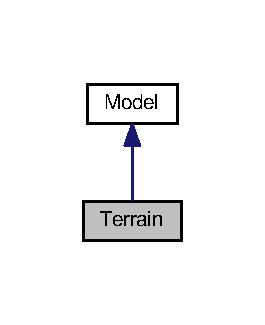
\includegraphics[width=127pt]{class_terrain__inherit__graph}
\end{center}
\end{figure}


Collaboration diagram for Terrain\+:\nopagebreak
\begin{figure}[H]
\begin{center}
\leavevmode
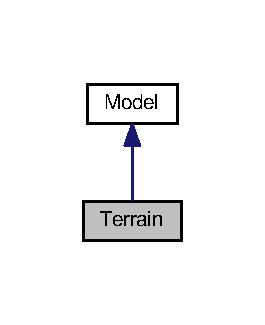
\includegraphics[width=127pt]{class_terrain__coll__graph}
\end{center}
\end{figure}
\subsection*{Public Member Functions}
\begin{DoxyCompactItemize}
\item 
\hyperlink{class_terrain_a7160a06ab07a86ed97d23374405e8ef6}{Terrain} ()
\item 
void \hyperlink{class_terrain_a69fd6856208f2d001035181ffb622a28}{generate\+Plane} (float width, float length)
\end{DoxyCompactItemize}
\subsection*{Additional Inherited Members}


\subsection{Constructor \& Destructor Documentation}
\index{Terrain@{Terrain}!Terrain@{Terrain}}
\index{Terrain@{Terrain}!Terrain@{Terrain}}
\subsubsection[{\texorpdfstring{Terrain()}{Terrain()}}]{\setlength{\rightskip}{0pt plus 5cm}Terrain\+::\+Terrain (
\begin{DoxyParamCaption}
{}
\end{DoxyParamCaption}
)}\hypertarget{class_terrain_a7160a06ab07a86ed97d23374405e8ef6}{}\label{class_terrain_a7160a06ab07a86ed97d23374405e8ef6}


\subsection{Member Function Documentation}
\index{Terrain@{Terrain}!generate\+Plane@{generate\+Plane}}
\index{generate\+Plane@{generate\+Plane}!Terrain@{Terrain}}
\subsubsection[{\texorpdfstring{generate\+Plane(float width, float length)}{generatePlane(float width, float length)}}]{\setlength{\rightskip}{0pt plus 5cm}void Terrain\+::generate\+Plane (
\begin{DoxyParamCaption}
\item[{float}]{width, }
\item[{float}]{length}
\end{DoxyParamCaption}
)}\hypertarget{class_terrain_a69fd6856208f2d001035181ffb622a28}{}\label{class_terrain_a69fd6856208f2d001035181ffb622a28}


The documentation for this class was generated from the following files\+:\begin{DoxyCompactItemize}
\item 
src/\hyperlink{_terrain_8h}{Terrain.\+h}\item 
src/\hyperlink{_terrain_8cpp}{Terrain.\+cpp}\end{DoxyCompactItemize}

\hypertarget{struct_turtle_1_1_transformation_set}{}\section{Turtle\+:\+:Transformation\+Set Struct Reference}
\label{struct_turtle_1_1_transformation_set}\index{Turtle\+::\+Transformation\+Set@{Turtle\+::\+Transformation\+Set}}


{\ttfamily \#include $<$Turtle.\+h$>$}

\subsection*{Public Attributes}
\begin{DoxyCompactItemize}
\item 
glm\+::vec3 \hyperlink{struct_turtle_1_1_transformation_set_a7e3907098175f964af8ffb88e1206f6a}{scale\+Vec}
\item 
glm\+::quat \hyperlink{struct_turtle_1_1_transformation_set_a7dffc2b5fb9511640e171b1fbdc4ac10}{orient\+Quat}
\item 
glm\+::vec3 \hyperlink{struct_turtle_1_1_transformation_set_aa6c7ef2414c618090e25d89574cc4af7}{transl\+Vec}
\end{DoxyCompactItemize}


\subsection{Member Data Documentation}
\index{Turtle\+::\+Transformation\+Set@{Turtle\+::\+Transformation\+Set}!orient\+Quat@{orient\+Quat}}
\index{orient\+Quat@{orient\+Quat}!Turtle\+::\+Transformation\+Set@{Turtle\+::\+Transformation\+Set}}
\subsubsection[{\texorpdfstring{orient\+Quat}{orientQuat}}]{\setlength{\rightskip}{0pt plus 5cm}glm\+::quat Turtle\+::\+Transformation\+Set\+::orient\+Quat}\hypertarget{struct_turtle_1_1_transformation_set_a7dffc2b5fb9511640e171b1fbdc4ac10}{}\label{struct_turtle_1_1_transformation_set_a7dffc2b5fb9511640e171b1fbdc4ac10}
\index{Turtle\+::\+Transformation\+Set@{Turtle\+::\+Transformation\+Set}!scale\+Vec@{scale\+Vec}}
\index{scale\+Vec@{scale\+Vec}!Turtle\+::\+Transformation\+Set@{Turtle\+::\+Transformation\+Set}}
\subsubsection[{\texorpdfstring{scale\+Vec}{scaleVec}}]{\setlength{\rightskip}{0pt plus 5cm}glm\+::vec3 Turtle\+::\+Transformation\+Set\+::scale\+Vec}\hypertarget{struct_turtle_1_1_transformation_set_a7e3907098175f964af8ffb88e1206f6a}{}\label{struct_turtle_1_1_transformation_set_a7e3907098175f964af8ffb88e1206f6a}
\index{Turtle\+::\+Transformation\+Set@{Turtle\+::\+Transformation\+Set}!transl\+Vec@{transl\+Vec}}
\index{transl\+Vec@{transl\+Vec}!Turtle\+::\+Transformation\+Set@{Turtle\+::\+Transformation\+Set}}
\subsubsection[{\texorpdfstring{transl\+Vec}{translVec}}]{\setlength{\rightskip}{0pt plus 5cm}glm\+::vec3 Turtle\+::\+Transformation\+Set\+::transl\+Vec}\hypertarget{struct_turtle_1_1_transformation_set_aa6c7ef2414c618090e25d89574cc4af7}{}\label{struct_turtle_1_1_transformation_set_aa6c7ef2414c618090e25d89574cc4af7}


The documentation for this struct was generated from the following file\+:\begin{DoxyCompactItemize}
\item 
src/\hyperlink{_turtle_8h}{Turtle.\+h}\end{DoxyCompactItemize}

\hypertarget{class_tree}{}\section{Tree Class Reference}
\label{class_tree}\index{Tree@{Tree}}


{\ttfamily \#include $<$Tree.\+h$>$}



Inheritance diagram for Tree\+:\nopagebreak
\begin{figure}[H]
\begin{center}
\leavevmode
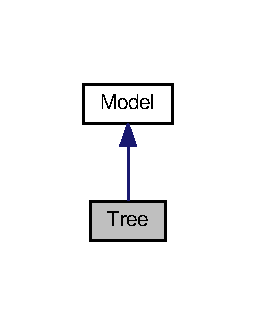
\includegraphics[width=123pt]{class_tree__inherit__graph}
\end{center}
\end{figure}


Collaboration diagram for Tree\+:\nopagebreak
\begin{figure}[H]
\begin{center}
\leavevmode
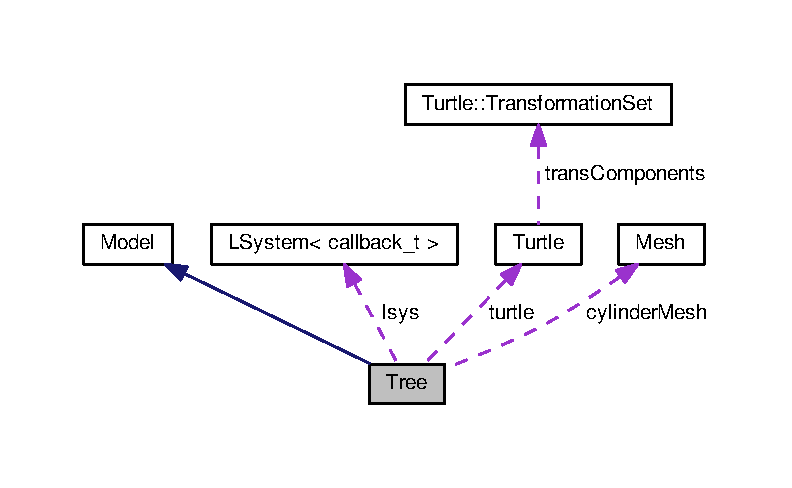
\includegraphics[width=350pt]{class_tree__coll__graph}
\end{center}
\end{figure}
\subsection*{Classes}
\begin{DoxyCompactItemize}
\item 
struct \hyperlink{struct_tree_1_1lsys_data}{lsys\+Data}
\end{DoxyCompactItemize}
\subsection*{Public Member Functions}
\begin{DoxyCompactItemize}
\item 
\hyperlink{class_tree_ab4ca65433a2e70d6fb468704a8f5d827}{Tree} (float n)
\end{DoxyCompactItemize}
\subsection*{Protected Types}
\begin{DoxyCompactItemize}
\item 
typedef void( \hyperlink{class_tree_a9978ae9b2adc867a50b92a110c6c44ef}{callback\+\_\+t}) (void $\ast$)
\end{DoxyCompactItemize}
\subsection*{Protected Attributes}
\begin{DoxyCompactItemize}
\item 
\hyperlink{class_l_system}{L\+System}$<$ \hyperlink{class_tree_a9978ae9b2adc867a50b92a110c6c44ef}{callback\+\_\+t} $>$ \hyperlink{class_tree_af10a84eb2afe93ab71dc1d7e12eb93fe}{lsys}
\item 
\hyperlink{class_turtle}{Turtle} \hyperlink{class_tree_a3eb5b35677be3847ed46da046564cf4c}{turtle}
\item 
\hyperlink{class_mesh}{Mesh} $\ast$ \hyperlink{class_tree_a27afed9bc6d61d5e7a83df806c42ba6b}{cylinder\+Mesh}
\item 
float \hyperlink{class_tree_a3dae13ef4932f05efe44e3c4bc002ad6}{angle}
\end{DoxyCompactItemize}


\subsection{Member Typedef Documentation}
\index{Tree@{Tree}!callback\+\_\+t@{callback\+\_\+t}}
\index{callback\+\_\+t@{callback\+\_\+t}!Tree@{Tree}}
\subsubsection[{\texorpdfstring{callback\+\_\+t}{callback_t}}]{\setlength{\rightskip}{0pt plus 5cm}typedef void( Tree\+::callback\+\_\+t) (void $\ast$)\hspace{0.3cm}{\ttfamily [protected]}}\hypertarget{class_tree_a9978ae9b2adc867a50b92a110c6c44ef}{}\label{class_tree_a9978ae9b2adc867a50b92a110c6c44ef}


\subsection{Constructor \& Destructor Documentation}
\index{Tree@{Tree}!Tree@{Tree}}
\index{Tree@{Tree}!Tree@{Tree}}
\subsubsection[{\texorpdfstring{Tree(float n)}{Tree(float n)}}]{\setlength{\rightskip}{0pt plus 5cm}Tree\+::\+Tree (
\begin{DoxyParamCaption}
\item[{float}]{n}
\end{DoxyParamCaption}
)}\hypertarget{class_tree_ab4ca65433a2e70d6fb468704a8f5d827}{}\label{class_tree_ab4ca65433a2e70d6fb468704a8f5d827}


\subsection{Member Data Documentation}
\index{Tree@{Tree}!angle@{angle}}
\index{angle@{angle}!Tree@{Tree}}
\subsubsection[{\texorpdfstring{angle}{angle}}]{\setlength{\rightskip}{0pt plus 5cm}float Tree\+::angle\hspace{0.3cm}{\ttfamily [protected]}}\hypertarget{class_tree_a3dae13ef4932f05efe44e3c4bc002ad6}{}\label{class_tree_a3dae13ef4932f05efe44e3c4bc002ad6}
\index{Tree@{Tree}!cylinder\+Mesh@{cylinder\+Mesh}}
\index{cylinder\+Mesh@{cylinder\+Mesh}!Tree@{Tree}}
\subsubsection[{\texorpdfstring{cylinder\+Mesh}{cylinderMesh}}]{\setlength{\rightskip}{0pt plus 5cm}{\bf Mesh}$\ast$ Tree\+::cylinder\+Mesh\hspace{0.3cm}{\ttfamily [protected]}}\hypertarget{class_tree_a27afed9bc6d61d5e7a83df806c42ba6b}{}\label{class_tree_a27afed9bc6d61d5e7a83df806c42ba6b}
\index{Tree@{Tree}!lsys@{lsys}}
\index{lsys@{lsys}!Tree@{Tree}}
\subsubsection[{\texorpdfstring{lsys}{lsys}}]{\setlength{\rightskip}{0pt plus 5cm}{\bf L\+System}$<${\bf callback\+\_\+t}$>$ Tree\+::lsys\hspace{0.3cm}{\ttfamily [protected]}}\hypertarget{class_tree_af10a84eb2afe93ab71dc1d7e12eb93fe}{}\label{class_tree_af10a84eb2afe93ab71dc1d7e12eb93fe}
\index{Tree@{Tree}!turtle@{turtle}}
\index{turtle@{turtle}!Tree@{Tree}}
\subsubsection[{\texorpdfstring{turtle}{turtle}}]{\setlength{\rightskip}{0pt plus 5cm}{\bf Turtle} Tree\+::turtle\hspace{0.3cm}{\ttfamily [protected]}}\hypertarget{class_tree_a3eb5b35677be3847ed46da046564cf4c}{}\label{class_tree_a3eb5b35677be3847ed46da046564cf4c}


The documentation for this class was generated from the following files\+:\begin{DoxyCompactItemize}
\item 
src/\hyperlink{_tree_8h}{Tree.\+h}\item 
src/\hyperlink{_tree_8cpp}{Tree.\+cpp}\end{DoxyCompactItemize}

\hypertarget{struct_para_tree_1_1_tree_params}{}\section{Para\+Tree\+:\+:Tree\+Params Struct Reference}
\label{struct_para_tree_1_1_tree_params}\index{Para\+Tree\+::\+Tree\+Params@{Para\+Tree\+::\+Tree\+Params}}


{\ttfamily \#include $<$Para\+Tree.\+h$>$}

\subsection*{Public Attributes}
\begin{DoxyCompactItemize}
\item 
float \hyperlink{struct_para_tree_1_1_tree_params_acdf6e36e58426bdb1289ebf2ab75502c}{r1}
\item 
float \hyperlink{struct_para_tree_1_1_tree_params_a87de942877435a9303395f43f7b55a91}{r2}
\item 
float \hyperlink{struct_para_tree_1_1_tree_params_ad7a978be36de75dd6faad5a25d6d47be}{a1}
\item 
float \hyperlink{struct_para_tree_1_1_tree_params_a4d3a22d7a87af7ae0191f2ec0970ad31}{a2}
\item 
float \hyperlink{struct_para_tree_1_1_tree_params_ada2709a5ff4b4dad887bf7522918e64a}{f1}
\item 
float \hyperlink{struct_para_tree_1_1_tree_params_aec341bcee27495140b7e05361626e9d8}{f2}
\item 
float \hyperlink{struct_para_tree_1_1_tree_params_acd7a09e825d636bcf13adf7259599cf3}{w0}
\item 
float \hyperlink{struct_para_tree_1_1_tree_params_a0ba9a10e66947fea4ad604701e16ba76}{q}
\item 
float \hyperlink{struct_para_tree_1_1_tree_params_ac10ef6a95bffabef0460ac27c478a67e}{e}
\item 
float \hyperlink{struct_para_tree_1_1_tree_params_a6e8de51864c4de420d6472a7107f2ee8}{min}
\item 
float \hyperlink{struct_para_tree_1_1_tree_params_a2d7f1c1e4b6163af7319cccd6615863f}{n}
\end{DoxyCompactItemize}


\subsection{Member Data Documentation}
\index{Para\+Tree\+::\+Tree\+Params@{Para\+Tree\+::\+Tree\+Params}!a1@{a1}}
\index{a1@{a1}!Para\+Tree\+::\+Tree\+Params@{Para\+Tree\+::\+Tree\+Params}}
\subsubsection[{\texorpdfstring{a1}{a1}}]{\setlength{\rightskip}{0pt plus 5cm}float Para\+Tree\+::\+Tree\+Params\+::a1}\hypertarget{struct_para_tree_1_1_tree_params_ad7a978be36de75dd6faad5a25d6d47be}{}\label{struct_para_tree_1_1_tree_params_ad7a978be36de75dd6faad5a25d6d47be}
\index{Para\+Tree\+::\+Tree\+Params@{Para\+Tree\+::\+Tree\+Params}!a2@{a2}}
\index{a2@{a2}!Para\+Tree\+::\+Tree\+Params@{Para\+Tree\+::\+Tree\+Params}}
\subsubsection[{\texorpdfstring{a2}{a2}}]{\setlength{\rightskip}{0pt plus 5cm}float Para\+Tree\+::\+Tree\+Params\+::a2}\hypertarget{struct_para_tree_1_1_tree_params_a4d3a22d7a87af7ae0191f2ec0970ad31}{}\label{struct_para_tree_1_1_tree_params_a4d3a22d7a87af7ae0191f2ec0970ad31}
\index{Para\+Tree\+::\+Tree\+Params@{Para\+Tree\+::\+Tree\+Params}!e@{e}}
\index{e@{e}!Para\+Tree\+::\+Tree\+Params@{Para\+Tree\+::\+Tree\+Params}}
\subsubsection[{\texorpdfstring{e}{e}}]{\setlength{\rightskip}{0pt plus 5cm}float Para\+Tree\+::\+Tree\+Params\+::e}\hypertarget{struct_para_tree_1_1_tree_params_ac10ef6a95bffabef0460ac27c478a67e}{}\label{struct_para_tree_1_1_tree_params_ac10ef6a95bffabef0460ac27c478a67e}
\index{Para\+Tree\+::\+Tree\+Params@{Para\+Tree\+::\+Tree\+Params}!f1@{f1}}
\index{f1@{f1}!Para\+Tree\+::\+Tree\+Params@{Para\+Tree\+::\+Tree\+Params}}
\subsubsection[{\texorpdfstring{f1}{f1}}]{\setlength{\rightskip}{0pt plus 5cm}float Para\+Tree\+::\+Tree\+Params\+::f1}\hypertarget{struct_para_tree_1_1_tree_params_ada2709a5ff4b4dad887bf7522918e64a}{}\label{struct_para_tree_1_1_tree_params_ada2709a5ff4b4dad887bf7522918e64a}
\index{Para\+Tree\+::\+Tree\+Params@{Para\+Tree\+::\+Tree\+Params}!f2@{f2}}
\index{f2@{f2}!Para\+Tree\+::\+Tree\+Params@{Para\+Tree\+::\+Tree\+Params}}
\subsubsection[{\texorpdfstring{f2}{f2}}]{\setlength{\rightskip}{0pt plus 5cm}float Para\+Tree\+::\+Tree\+Params\+::f2}\hypertarget{struct_para_tree_1_1_tree_params_aec341bcee27495140b7e05361626e9d8}{}\label{struct_para_tree_1_1_tree_params_aec341bcee27495140b7e05361626e9d8}
\index{Para\+Tree\+::\+Tree\+Params@{Para\+Tree\+::\+Tree\+Params}!min@{min}}
\index{min@{min}!Para\+Tree\+::\+Tree\+Params@{Para\+Tree\+::\+Tree\+Params}}
\subsubsection[{\texorpdfstring{min}{min}}]{\setlength{\rightskip}{0pt plus 5cm}float Para\+Tree\+::\+Tree\+Params\+::min}\hypertarget{struct_para_tree_1_1_tree_params_a6e8de51864c4de420d6472a7107f2ee8}{}\label{struct_para_tree_1_1_tree_params_a6e8de51864c4de420d6472a7107f2ee8}
\index{Para\+Tree\+::\+Tree\+Params@{Para\+Tree\+::\+Tree\+Params}!n@{n}}
\index{n@{n}!Para\+Tree\+::\+Tree\+Params@{Para\+Tree\+::\+Tree\+Params}}
\subsubsection[{\texorpdfstring{n}{n}}]{\setlength{\rightskip}{0pt plus 5cm}float Para\+Tree\+::\+Tree\+Params\+::n}\hypertarget{struct_para_tree_1_1_tree_params_a2d7f1c1e4b6163af7319cccd6615863f}{}\label{struct_para_tree_1_1_tree_params_a2d7f1c1e4b6163af7319cccd6615863f}
\index{Para\+Tree\+::\+Tree\+Params@{Para\+Tree\+::\+Tree\+Params}!q@{q}}
\index{q@{q}!Para\+Tree\+::\+Tree\+Params@{Para\+Tree\+::\+Tree\+Params}}
\subsubsection[{\texorpdfstring{q}{q}}]{\setlength{\rightskip}{0pt plus 5cm}float Para\+Tree\+::\+Tree\+Params\+::q}\hypertarget{struct_para_tree_1_1_tree_params_a0ba9a10e66947fea4ad604701e16ba76}{}\label{struct_para_tree_1_1_tree_params_a0ba9a10e66947fea4ad604701e16ba76}
\index{Para\+Tree\+::\+Tree\+Params@{Para\+Tree\+::\+Tree\+Params}!r1@{r1}}
\index{r1@{r1}!Para\+Tree\+::\+Tree\+Params@{Para\+Tree\+::\+Tree\+Params}}
\subsubsection[{\texorpdfstring{r1}{r1}}]{\setlength{\rightskip}{0pt plus 5cm}float Para\+Tree\+::\+Tree\+Params\+::r1}\hypertarget{struct_para_tree_1_1_tree_params_acdf6e36e58426bdb1289ebf2ab75502c}{}\label{struct_para_tree_1_1_tree_params_acdf6e36e58426bdb1289ebf2ab75502c}
\index{Para\+Tree\+::\+Tree\+Params@{Para\+Tree\+::\+Tree\+Params}!r2@{r2}}
\index{r2@{r2}!Para\+Tree\+::\+Tree\+Params@{Para\+Tree\+::\+Tree\+Params}}
\subsubsection[{\texorpdfstring{r2}{r2}}]{\setlength{\rightskip}{0pt plus 5cm}float Para\+Tree\+::\+Tree\+Params\+::r2}\hypertarget{struct_para_tree_1_1_tree_params_a87de942877435a9303395f43f7b55a91}{}\label{struct_para_tree_1_1_tree_params_a87de942877435a9303395f43f7b55a91}
\index{Para\+Tree\+::\+Tree\+Params@{Para\+Tree\+::\+Tree\+Params}!w0@{w0}}
\index{w0@{w0}!Para\+Tree\+::\+Tree\+Params@{Para\+Tree\+::\+Tree\+Params}}
\subsubsection[{\texorpdfstring{w0}{w0}}]{\setlength{\rightskip}{0pt plus 5cm}float Para\+Tree\+::\+Tree\+Params\+::w0}\hypertarget{struct_para_tree_1_1_tree_params_acd7a09e825d636bcf13adf7259599cf3}{}\label{struct_para_tree_1_1_tree_params_acd7a09e825d636bcf13adf7259599cf3}


The documentation for this struct was generated from the following file\+:\begin{DoxyCompactItemize}
\item 
src/\hyperlink{_para_tree_8h}{Para\+Tree.\+h}\end{DoxyCompactItemize}

\hypertarget{class_turtle}{}\section{Turtle Class Reference}
\label{class_turtle}\index{Turtle@{Turtle}}


{\ttfamily \#include $<$Turtle.\+h$>$}



Collaboration diagram for Turtle\+:\nopagebreak
\begin{figure}[H]
\begin{center}
\leavevmode
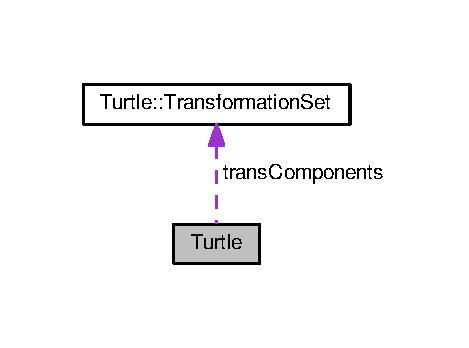
\includegraphics[width=225pt]{class_turtle__coll__graph}
\end{center}
\end{figure}
\subsection*{Classes}
\begin{DoxyCompactItemize}
\item 
struct \hyperlink{struct_turtle_1_1_transformation_set}{Transformation\+Set}
\end{DoxyCompactItemize}
\subsection*{Public Member Functions}
\begin{DoxyCompactItemize}
\item 
\hyperlink{class_turtle_a1610c37c2e750169f25b074e62db755d}{Turtle} ()
\item 
void \hyperlink{class_turtle_a52f47f3d3f660de0f425eb15f51f57a9}{scale} (glm\+::vec3 s)
\item 
void \hyperlink{class_turtle_a6365b6bf9e1b63ad7067623704f96b7b}{rotate} (float angle, glm\+::vec3 axis)
\item 
void \hyperlink{class_turtle_a7247837e1e7f34053ceba1a8ba35f792}{turn} (float angle)
\item 
void \hyperlink{class_turtle_af612347a6ccf6020a86e14b0bad76d29}{pitch} (float angle)
\item 
void \hyperlink{class_turtle_a12f15e7d93be8f46c4af5b2815cad994}{roll} (float angle)
\item 
void \hyperlink{class_turtle_ad02ab2d43a59a84c79ecee57dbe7d1dc}{forward} (float t)
\item 
void \hyperlink{class_turtle_a83d7165e83a6a4c82e54f4e918163eab}{set\+Length} (float l)
\item 
void \hyperlink{class_turtle_ab106e2a57335119d0f307d19633f682b}{set\+Width} (float w)
\item 
glm\+::mat4 \hyperlink{class_turtle_a29c13ff42b394345c21dad4c84022bcc}{get\+Matrix} ()
\item 
void \hyperlink{class_turtle_a9562a857f3d87a742a28f2b3bca4995c}{push} ()
\item 
void \hyperlink{class_turtle_a1967bcd0701b9fbab2d312194a575703}{pop} ()
\end{DoxyCompactItemize}
\subsection*{Protected Attributes}
\begin{DoxyCompactItemize}
\item 
struct \hyperlink{struct_turtle_1_1_transformation_set}{Turtle\+::\+Transformation\+Set} \hyperlink{class_turtle_a1c9daa775c36e1a3414522488780f686}{trans\+Components}
\item 
stack$<$ \hyperlink{struct_turtle_1_1_transformation_set}{Transformation\+Set} $>$ \hyperlink{class_turtle_ab881dbccdf3460b344ff3bd724d1cf06}{trans\+Stack}
\end{DoxyCompactItemize}


\subsection{Constructor \& Destructor Documentation}
\index{Turtle@{Turtle}!Turtle@{Turtle}}
\index{Turtle@{Turtle}!Turtle@{Turtle}}
\subsubsection[{\texorpdfstring{Turtle()}{Turtle()}}]{\setlength{\rightskip}{0pt plus 5cm}Turtle\+::\+Turtle (
\begin{DoxyParamCaption}
{}
\end{DoxyParamCaption}
)\hspace{0.3cm}{\ttfamily [inline]}}\hypertarget{class_turtle_a1610c37c2e750169f25b074e62db755d}{}\label{class_turtle_a1610c37c2e750169f25b074e62db755d}


\subsection{Member Function Documentation}
\index{Turtle@{Turtle}!forward@{forward}}
\index{forward@{forward}!Turtle@{Turtle}}
\subsubsection[{\texorpdfstring{forward(float t)}{forward(float t)}}]{\setlength{\rightskip}{0pt plus 5cm}void Turtle\+::forward (
\begin{DoxyParamCaption}
\item[{float}]{t}
\end{DoxyParamCaption}
)\hspace{0.3cm}{\ttfamily [inline]}}\hypertarget{class_turtle_ad02ab2d43a59a84c79ecee57dbe7d1dc}{}\label{class_turtle_ad02ab2d43a59a84c79ecee57dbe7d1dc}
\index{Turtle@{Turtle}!get\+Matrix@{get\+Matrix}}
\index{get\+Matrix@{get\+Matrix}!Turtle@{Turtle}}
\subsubsection[{\texorpdfstring{get\+Matrix()}{getMatrix()}}]{\setlength{\rightskip}{0pt plus 5cm}glm\+::mat4 Turtle\+::get\+Matrix (
\begin{DoxyParamCaption}
{}
\end{DoxyParamCaption}
)\hspace{0.3cm}{\ttfamily [inline]}}\hypertarget{class_turtle_a29c13ff42b394345c21dad4c84022bcc}{}\label{class_turtle_a29c13ff42b394345c21dad4c84022bcc}
\index{Turtle@{Turtle}!pitch@{pitch}}
\index{pitch@{pitch}!Turtle@{Turtle}}
\subsubsection[{\texorpdfstring{pitch(float angle)}{pitch(float angle)}}]{\setlength{\rightskip}{0pt plus 5cm}void Turtle\+::pitch (
\begin{DoxyParamCaption}
\item[{float}]{angle}
\end{DoxyParamCaption}
)\hspace{0.3cm}{\ttfamily [inline]}}\hypertarget{class_turtle_af612347a6ccf6020a86e14b0bad76d29}{}\label{class_turtle_af612347a6ccf6020a86e14b0bad76d29}
\index{Turtle@{Turtle}!pop@{pop}}
\index{pop@{pop}!Turtle@{Turtle}}
\subsubsection[{\texorpdfstring{pop()}{pop()}}]{\setlength{\rightskip}{0pt plus 5cm}void Turtle\+::pop (
\begin{DoxyParamCaption}
{}
\end{DoxyParamCaption}
)\hspace{0.3cm}{\ttfamily [inline]}}\hypertarget{class_turtle_a1967bcd0701b9fbab2d312194a575703}{}\label{class_turtle_a1967bcd0701b9fbab2d312194a575703}
\index{Turtle@{Turtle}!push@{push}}
\index{push@{push}!Turtle@{Turtle}}
\subsubsection[{\texorpdfstring{push()}{push()}}]{\setlength{\rightskip}{0pt plus 5cm}void Turtle\+::push (
\begin{DoxyParamCaption}
{}
\end{DoxyParamCaption}
)\hspace{0.3cm}{\ttfamily [inline]}}\hypertarget{class_turtle_a9562a857f3d87a742a28f2b3bca4995c}{}\label{class_turtle_a9562a857f3d87a742a28f2b3bca4995c}
\index{Turtle@{Turtle}!roll@{roll}}
\index{roll@{roll}!Turtle@{Turtle}}
\subsubsection[{\texorpdfstring{roll(float angle)}{roll(float angle)}}]{\setlength{\rightskip}{0pt plus 5cm}void Turtle\+::roll (
\begin{DoxyParamCaption}
\item[{float}]{angle}
\end{DoxyParamCaption}
)\hspace{0.3cm}{\ttfamily [inline]}}\hypertarget{class_turtle_a12f15e7d93be8f46c4af5b2815cad994}{}\label{class_turtle_a12f15e7d93be8f46c4af5b2815cad994}
\index{Turtle@{Turtle}!rotate@{rotate}}
\index{rotate@{rotate}!Turtle@{Turtle}}
\subsubsection[{\texorpdfstring{rotate(float angle, glm\+::vec3 axis)}{rotate(float angle, glm::vec3 axis)}}]{\setlength{\rightskip}{0pt plus 5cm}void Turtle\+::rotate (
\begin{DoxyParamCaption}
\item[{float}]{angle, }
\item[{glm\+::vec3}]{axis}
\end{DoxyParamCaption}
)\hspace{0.3cm}{\ttfamily [inline]}}\hypertarget{class_turtle_a6365b6bf9e1b63ad7067623704f96b7b}{}\label{class_turtle_a6365b6bf9e1b63ad7067623704f96b7b}
\index{Turtle@{Turtle}!scale@{scale}}
\index{scale@{scale}!Turtle@{Turtle}}
\subsubsection[{\texorpdfstring{scale(glm\+::vec3 s)}{scale(glm::vec3 s)}}]{\setlength{\rightskip}{0pt plus 5cm}void Turtle\+::scale (
\begin{DoxyParamCaption}
\item[{glm\+::vec3}]{s}
\end{DoxyParamCaption}
)\hspace{0.3cm}{\ttfamily [inline]}}\hypertarget{class_turtle_a52f47f3d3f660de0f425eb15f51f57a9}{}\label{class_turtle_a52f47f3d3f660de0f425eb15f51f57a9}
\index{Turtle@{Turtle}!set\+Length@{set\+Length}}
\index{set\+Length@{set\+Length}!Turtle@{Turtle}}
\subsubsection[{\texorpdfstring{set\+Length(float l)}{setLength(float l)}}]{\setlength{\rightskip}{0pt plus 5cm}void Turtle\+::set\+Length (
\begin{DoxyParamCaption}
\item[{float}]{l}
\end{DoxyParamCaption}
)\hspace{0.3cm}{\ttfamily [inline]}}\hypertarget{class_turtle_a83d7165e83a6a4c82e54f4e918163eab}{}\label{class_turtle_a83d7165e83a6a4c82e54f4e918163eab}
\index{Turtle@{Turtle}!set\+Width@{set\+Width}}
\index{set\+Width@{set\+Width}!Turtle@{Turtle}}
\subsubsection[{\texorpdfstring{set\+Width(float w)}{setWidth(float w)}}]{\setlength{\rightskip}{0pt plus 5cm}void Turtle\+::set\+Width (
\begin{DoxyParamCaption}
\item[{float}]{w}
\end{DoxyParamCaption}
)\hspace{0.3cm}{\ttfamily [inline]}}\hypertarget{class_turtle_ab106e2a57335119d0f307d19633f682b}{}\label{class_turtle_ab106e2a57335119d0f307d19633f682b}
\index{Turtle@{Turtle}!turn@{turn}}
\index{turn@{turn}!Turtle@{Turtle}}
\subsubsection[{\texorpdfstring{turn(float angle)}{turn(float angle)}}]{\setlength{\rightskip}{0pt plus 5cm}void Turtle\+::turn (
\begin{DoxyParamCaption}
\item[{float}]{angle}
\end{DoxyParamCaption}
)\hspace{0.3cm}{\ttfamily [inline]}}\hypertarget{class_turtle_a7247837e1e7f34053ceba1a8ba35f792}{}\label{class_turtle_a7247837e1e7f34053ceba1a8ba35f792}


\subsection{Member Data Documentation}
\index{Turtle@{Turtle}!trans\+Components@{trans\+Components}}
\index{trans\+Components@{trans\+Components}!Turtle@{Turtle}}
\subsubsection[{\texorpdfstring{trans\+Components}{transComponents}}]{\setlength{\rightskip}{0pt plus 5cm}struct {\bf Turtle\+::\+Transformation\+Set}  Turtle\+::trans\+Components\hspace{0.3cm}{\ttfamily [protected]}}\hypertarget{class_turtle_a1c9daa775c36e1a3414522488780f686}{}\label{class_turtle_a1c9daa775c36e1a3414522488780f686}
\index{Turtle@{Turtle}!trans\+Stack@{trans\+Stack}}
\index{trans\+Stack@{trans\+Stack}!Turtle@{Turtle}}
\subsubsection[{\texorpdfstring{trans\+Stack}{transStack}}]{\setlength{\rightskip}{0pt plus 5cm}stack$<${\bf Transformation\+Set}$>$ Turtle\+::trans\+Stack\hspace{0.3cm}{\ttfamily [protected]}}\hypertarget{class_turtle_ab881dbccdf3460b344ff3bd724d1cf06}{}\label{class_turtle_ab881dbccdf3460b344ff3bd724d1cf06}


The documentation for this class was generated from the following file\+:\begin{DoxyCompactItemize}
\item 
src/\hyperlink{_turtle_8h}{Turtle.\+h}\end{DoxyCompactItemize}

\hypertarget{class_u_i_1_1_u_i_base}{}\section{UI\+:\+:U\+I\+Base Class Reference}
\label{class_u_i_1_1_u_i_base}\index{U\+I\+::\+U\+I\+Base@{U\+I\+::\+U\+I\+Base}}


{\ttfamily \#include $<$U\+I.\+h$>$}



Inheritance diagram for UI\+:\+:U\+I\+Base\+:\nopagebreak
\begin{figure}[H]
\begin{center}
\leavevmode
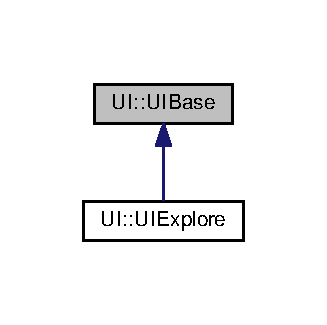
\includegraphics[width=157pt]{class_u_i_1_1_u_i_base__inherit__graph}
\end{center}
\end{figure}
\subsection*{Public Member Functions}
\begin{DoxyCompactItemize}
\item 
virtual void \hyperlink{class_u_i_1_1_u_i_base_a795c1f2aad98bf128515a8033af63aa7}{set\+Active} ()
\end{DoxyCompactItemize}
\subsection*{Static Public Member Functions}
\begin{DoxyCompactItemize}
\item 
static void \hyperlink{class_u_i_1_1_u_i_base_a5f82346e3b961a1cec579692d02dfee7}{on\+Key\+Dispatcher} (G\+L\+F\+Wwindow $\ast$\hyperlink{namespace_u_i_ac05ba8c1833c723ee85c762399654d3e}{window}, int key, int scancode, int action, int mods)
\item 
static void \hyperlink{class_u_i_1_1_u_i_base_a40fb9f20db942544fe2b8ae8436524a2}{on\+Mouse\+Button\+Dispatcher} (G\+L\+F\+Wwindow $\ast$\hyperlink{namespace_u_i_ac05ba8c1833c723ee85c762399654d3e}{window}, int button, int action, int mods)
\item 
static void \hyperlink{class_u_i_1_1_u_i_base_a3de0a954520fd587e10fa47f93d8a937}{on\+Cursor\+Move\+Dispatcher} (G\+L\+F\+Wwindow $\ast$\hyperlink{namespace_u_i_ac05ba8c1833c723ee85c762399654d3e}{window}, double xpos, double ypos)
\item 
static void \hyperlink{class_u_i_1_1_u_i_base_af3d73d8afcd634826fc28e7b831f67b8}{on\+Resize\+Dispatcher} (G\+L\+F\+Wwindow $\ast$\hyperlink{namespace_u_i_ac05ba8c1833c723ee85c762399654d3e}{window}, int width, int height)
\end{DoxyCompactItemize}


\subsection{Member Function Documentation}
\index{U\+I\+::\+U\+I\+Base@{U\+I\+::\+U\+I\+Base}!on\+Cursor\+Move\+Dispatcher@{on\+Cursor\+Move\+Dispatcher}}
\index{on\+Cursor\+Move\+Dispatcher@{on\+Cursor\+Move\+Dispatcher}!U\+I\+::\+U\+I\+Base@{U\+I\+::\+U\+I\+Base}}
\subsubsection[{\texorpdfstring{on\+Cursor\+Move\+Dispatcher(\+G\+L\+F\+Wwindow $\ast$window, double xpos, double ypos)}{onCursorMoveDispatcher(GLFWwindow *window, double xpos, double ypos)}}]{\setlength{\rightskip}{0pt plus 5cm}static void U\+I\+::\+U\+I\+Base\+::on\+Cursor\+Move\+Dispatcher (
\begin{DoxyParamCaption}
\item[{G\+L\+F\+Wwindow $\ast$}]{window, }
\item[{double}]{xpos, }
\item[{double}]{ypos}
\end{DoxyParamCaption}
)\hspace{0.3cm}{\ttfamily [inline]}, {\ttfamily [static]}}\hypertarget{class_u_i_1_1_u_i_base_a3de0a954520fd587e10fa47f93d8a937}{}\label{class_u_i_1_1_u_i_base_a3de0a954520fd587e10fa47f93d8a937}
\index{U\+I\+::\+U\+I\+Base@{U\+I\+::\+U\+I\+Base}!on\+Key\+Dispatcher@{on\+Key\+Dispatcher}}
\index{on\+Key\+Dispatcher@{on\+Key\+Dispatcher}!U\+I\+::\+U\+I\+Base@{U\+I\+::\+U\+I\+Base}}
\subsubsection[{\texorpdfstring{on\+Key\+Dispatcher(\+G\+L\+F\+Wwindow $\ast$window, int key, int scancode, int action, int mods)}{onKeyDispatcher(GLFWwindow *window, int key, int scancode, int action, int mods)}}]{\setlength{\rightskip}{0pt plus 5cm}static void U\+I\+::\+U\+I\+Base\+::on\+Key\+Dispatcher (
\begin{DoxyParamCaption}
\item[{G\+L\+F\+Wwindow $\ast$}]{window, }
\item[{int}]{key, }
\item[{int}]{scancode, }
\item[{int}]{action, }
\item[{int}]{mods}
\end{DoxyParamCaption}
)\hspace{0.3cm}{\ttfamily [inline]}, {\ttfamily [static]}}\hypertarget{class_u_i_1_1_u_i_base_a5f82346e3b961a1cec579692d02dfee7}{}\label{class_u_i_1_1_u_i_base_a5f82346e3b961a1cec579692d02dfee7}
\index{U\+I\+::\+U\+I\+Base@{U\+I\+::\+U\+I\+Base}!on\+Mouse\+Button\+Dispatcher@{on\+Mouse\+Button\+Dispatcher}}
\index{on\+Mouse\+Button\+Dispatcher@{on\+Mouse\+Button\+Dispatcher}!U\+I\+::\+U\+I\+Base@{U\+I\+::\+U\+I\+Base}}
\subsubsection[{\texorpdfstring{on\+Mouse\+Button\+Dispatcher(\+G\+L\+F\+Wwindow $\ast$window, int button, int action, int mods)}{onMouseButtonDispatcher(GLFWwindow *window, int button, int action, int mods)}}]{\setlength{\rightskip}{0pt plus 5cm}static void U\+I\+::\+U\+I\+Base\+::on\+Mouse\+Button\+Dispatcher (
\begin{DoxyParamCaption}
\item[{G\+L\+F\+Wwindow $\ast$}]{window, }
\item[{int}]{button, }
\item[{int}]{action, }
\item[{int}]{mods}
\end{DoxyParamCaption}
)\hspace{0.3cm}{\ttfamily [inline]}, {\ttfamily [static]}}\hypertarget{class_u_i_1_1_u_i_base_a40fb9f20db942544fe2b8ae8436524a2}{}\label{class_u_i_1_1_u_i_base_a40fb9f20db942544fe2b8ae8436524a2}
\index{U\+I\+::\+U\+I\+Base@{U\+I\+::\+U\+I\+Base}!on\+Resize\+Dispatcher@{on\+Resize\+Dispatcher}}
\index{on\+Resize\+Dispatcher@{on\+Resize\+Dispatcher}!U\+I\+::\+U\+I\+Base@{U\+I\+::\+U\+I\+Base}}
\subsubsection[{\texorpdfstring{on\+Resize\+Dispatcher(\+G\+L\+F\+Wwindow $\ast$window, int width, int height)}{onResizeDispatcher(GLFWwindow *window, int width, int height)}}]{\setlength{\rightskip}{0pt plus 5cm}static void U\+I\+::\+U\+I\+Base\+::on\+Resize\+Dispatcher (
\begin{DoxyParamCaption}
\item[{G\+L\+F\+Wwindow $\ast$}]{window, }
\item[{int}]{width, }
\item[{int}]{height}
\end{DoxyParamCaption}
)\hspace{0.3cm}{\ttfamily [inline]}, {\ttfamily [static]}}\hypertarget{class_u_i_1_1_u_i_base_af3d73d8afcd634826fc28e7b831f67b8}{}\label{class_u_i_1_1_u_i_base_af3d73d8afcd634826fc28e7b831f67b8}
\index{U\+I\+::\+U\+I\+Base@{U\+I\+::\+U\+I\+Base}!set\+Active@{set\+Active}}
\index{set\+Active@{set\+Active}!U\+I\+::\+U\+I\+Base@{U\+I\+::\+U\+I\+Base}}
\subsubsection[{\texorpdfstring{set\+Active()}{setActive()}}]{\setlength{\rightskip}{0pt plus 5cm}virtual void U\+I\+::\+U\+I\+Base\+::set\+Active (
\begin{DoxyParamCaption}
{}
\end{DoxyParamCaption}
)\hspace{0.3cm}{\ttfamily [inline]}, {\ttfamily [virtual]}}\hypertarget{class_u_i_1_1_u_i_base_a795c1f2aad98bf128515a8033af63aa7}{}\label{class_u_i_1_1_u_i_base_a795c1f2aad98bf128515a8033af63aa7}


The documentation for this class was generated from the following files\+:\begin{DoxyCompactItemize}
\item 
src/\hyperlink{_u_i_8h}{U\+I.\+h}\item 
src/\hyperlink{_u_i_8cpp}{U\+I.\+cpp}\end{DoxyCompactItemize}

\hypertarget{class_u_i_1_1_u_i_explore}{}\section{UI\+:\+:U\+I\+Explore Class Reference}
\label{class_u_i_1_1_u_i_explore}\index{U\+I\+::\+U\+I\+Explore@{U\+I\+::\+U\+I\+Explore}}


{\ttfamily \#include $<$U\+I.\+h$>$}



Inheritance diagram for UI\+:\+:U\+I\+Explore\+:\nopagebreak
\begin{figure}[H]
\begin{center}
\leavevmode
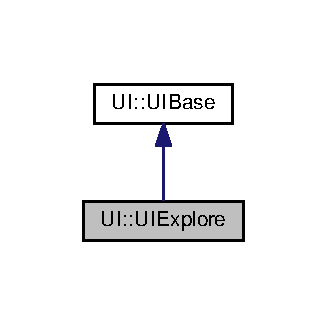
\includegraphics[width=157pt]{class_u_i_1_1_u_i_explore__inherit__graph}
\end{center}
\end{figure}


Collaboration diagram for UI\+:\+:U\+I\+Explore\+:\nopagebreak
\begin{figure}[H]
\begin{center}
\leavevmode
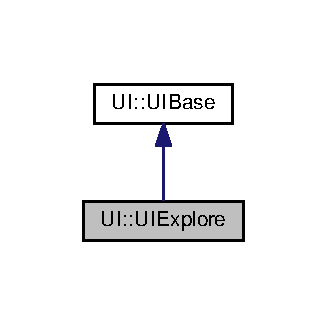
\includegraphics[width=157pt]{class_u_i_1_1_u_i_explore__coll__graph}
\end{center}
\end{figure}
\subsection*{Additional Inherited Members}


The documentation for this class was generated from the following files\+:\begin{DoxyCompactItemize}
\item 
src/\hyperlink{_u_i_8h}{U\+I.\+h}\item 
src/\hyperlink{_u_i_8cpp}{U\+I.\+cpp}\end{DoxyCompactItemize}

\hypertarget{struct_vertex}{}\section{Vertex Struct Reference}
\label{struct_vertex}\index{Vertex@{Vertex}}


{\ttfamily \#include $<$Vertex.\+h$>$}

\subsection*{Public Attributes}
\begin{DoxyCompactItemize}
\item 
glm\+::vec3 \hyperlink{struct_vertex_a030819fdc241743bbd3e180a6b132ed3}{position}
\item 
glm\+::vec3 \hyperlink{struct_vertex_a3aa35fe84025ecf1acccb5f65f5577fd}{normal}
\end{DoxyCompactItemize}


\subsection{Member Data Documentation}
\index{Vertex@{Vertex}!normal@{normal}}
\index{normal@{normal}!Vertex@{Vertex}}
\subsubsection[{\texorpdfstring{normal}{normal}}]{\setlength{\rightskip}{0pt plus 5cm}glm\+::vec3 Vertex\+::normal}\hypertarget{struct_vertex_a3aa35fe84025ecf1acccb5f65f5577fd}{}\label{struct_vertex_a3aa35fe84025ecf1acccb5f65f5577fd}
\index{Vertex@{Vertex}!position@{position}}
\index{position@{position}!Vertex@{Vertex}}
\subsubsection[{\texorpdfstring{position}{position}}]{\setlength{\rightskip}{0pt plus 5cm}glm\+::vec3 Vertex\+::position}\hypertarget{struct_vertex_a030819fdc241743bbd3e180a6b132ed3}{}\label{struct_vertex_a030819fdc241743bbd3e180a6b132ed3}


The documentation for this struct was generated from the following file\+:\begin{DoxyCompactItemize}
\item 
src/\hyperlink{_vertex_8h}{Vertex.\+h}\end{DoxyCompactItemize}

\hypertarget{class_world}{}\section{World Class Reference}
\label{class_world}\index{World@{World}}


{\ttfamily \#include $<$World.\+h$>$}



Collaboration diagram for World\+:\nopagebreak
\begin{figure}[H]
\begin{center}
\leavevmode
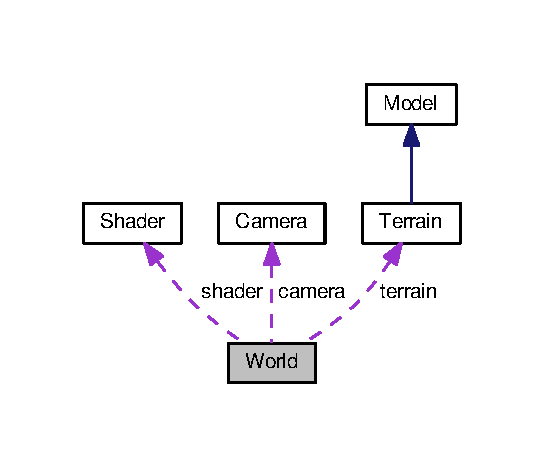
\includegraphics[width=261pt]{class_world__coll__graph}
\end{center}
\end{figure}
\subsection*{Public Member Functions}
\begin{DoxyCompactItemize}
\item 
\hyperlink{class_world_afa39d4e6f714a7a3691ac0c656f5e8a8}{World} ()
\item 
void \hyperlink{class_world_ab51a17ccbb108616daacd0c34973dc8d}{draw} ()
\end{DoxyCompactItemize}
\subsection*{Public Attributes}
\begin{DoxyCompactItemize}
\item 
\hyperlink{class_terrain}{Terrain} \hyperlink{class_world_a7a580c4cbd8085edcd2fea787331ff57}{terrain}
\item 
\hyperlink{class_camera}{Camera} \hyperlink{class_world_afef936319256711ddc3f38b2c1ec521f}{camera}
\end{DoxyCompactItemize}
\subsection*{Protected Attributes}
\begin{DoxyCompactItemize}
\item 
const char $\ast$ \hyperlink{class_world_a9333bdf78ba2581b9f3cc6295b672072}{T\+E\+R\+R\+A\+I\+N\+\_\+\+P\+A\+T\+H\+\_\+\+H\+E\+I\+G\+H\+T\+M\+AP} = \char`\"{}/res/heightmap\+\_\+lores.\+png\char`\"{}
\item 
const char $\ast$ \hyperlink{class_world_a51982474b4db4216dd2643e0208b3827}{T\+E\+R\+R\+A\+I\+N\+\_\+\+P\+A\+T\+H\+\_\+\+C\+O\+L\+OR} = \char`\"{}/res/colour\+\_\+lores.\+png\char`\"{}
\item 
G\+L\+F\+Wwindow $\ast$ \hyperlink{class_world_a948668ffc237256daba819fd35c5ab68}{window}
\item 
\hyperlink{class_shader}{Shader} \hyperlink{class_world_a342cc7caee93c7676ddc03b48f7984b8}{shader}
\item 
G\+Lint \hyperlink{class_world_ac64b16c23059bb26d597806daa516cbe}{uni\+\_\+view\+Mat}
\item 
G\+Lint \hyperlink{class_world_ab988aa593cf46e234282796eab0b6c92}{uni\+\_\+proj\+Mat}
\item 
list$<$ \hyperlink{class_model}{Model} $\ast$ $>$ \hyperlink{class_world_afa3d9082fd84060ff8c7fc42ed7ed8a2}{models}
\end{DoxyCompactItemize}


\subsection{Constructor \& Destructor Documentation}
\index{World@{World}!World@{World}}
\index{World@{World}!World@{World}}
\subsubsection[{\texorpdfstring{World()}{World()}}]{\setlength{\rightskip}{0pt plus 5cm}World\+::\+World (
\begin{DoxyParamCaption}
{}
\end{DoxyParamCaption}
)}\hypertarget{class_world_afa39d4e6f714a7a3691ac0c656f5e8a8}{}\label{class_world_afa39d4e6f714a7a3691ac0c656f5e8a8}


\subsection{Member Function Documentation}
\index{World@{World}!draw@{draw}}
\index{draw@{draw}!World@{World}}
\subsubsection[{\texorpdfstring{draw()}{draw()}}]{\setlength{\rightskip}{0pt plus 5cm}void World\+::draw (
\begin{DoxyParamCaption}
{}
\end{DoxyParamCaption}
)}\hypertarget{class_world_ab51a17ccbb108616daacd0c34973dc8d}{}\label{class_world_ab51a17ccbb108616daacd0c34973dc8d}


\subsection{Member Data Documentation}
\index{World@{World}!camera@{camera}}
\index{camera@{camera}!World@{World}}
\subsubsection[{\texorpdfstring{camera}{camera}}]{\setlength{\rightskip}{0pt plus 5cm}{\bf Camera} World\+::camera}\hypertarget{class_world_afef936319256711ddc3f38b2c1ec521f}{}\label{class_world_afef936319256711ddc3f38b2c1ec521f}
\index{World@{World}!models@{models}}
\index{models@{models}!World@{World}}
\subsubsection[{\texorpdfstring{models}{models}}]{\setlength{\rightskip}{0pt plus 5cm}list$<${\bf Model}$\ast$$>$ World\+::models\hspace{0.3cm}{\ttfamily [protected]}}\hypertarget{class_world_afa3d9082fd84060ff8c7fc42ed7ed8a2}{}\label{class_world_afa3d9082fd84060ff8c7fc42ed7ed8a2}
\index{World@{World}!shader@{shader}}
\index{shader@{shader}!World@{World}}
\subsubsection[{\texorpdfstring{shader}{shader}}]{\setlength{\rightskip}{0pt plus 5cm}{\bf Shader} World\+::shader\hspace{0.3cm}{\ttfamily [protected]}}\hypertarget{class_world_a342cc7caee93c7676ddc03b48f7984b8}{}\label{class_world_a342cc7caee93c7676ddc03b48f7984b8}
\index{World@{World}!terrain@{terrain}}
\index{terrain@{terrain}!World@{World}}
\subsubsection[{\texorpdfstring{terrain}{terrain}}]{\setlength{\rightskip}{0pt plus 5cm}{\bf Terrain} World\+::terrain}\hypertarget{class_world_a7a580c4cbd8085edcd2fea787331ff57}{}\label{class_world_a7a580c4cbd8085edcd2fea787331ff57}
\index{World@{World}!T\+E\+R\+R\+A\+I\+N\+\_\+\+P\+A\+T\+H\+\_\+\+C\+O\+L\+OR@{T\+E\+R\+R\+A\+I\+N\+\_\+\+P\+A\+T\+H\+\_\+\+C\+O\+L\+OR}}
\index{T\+E\+R\+R\+A\+I\+N\+\_\+\+P\+A\+T\+H\+\_\+\+C\+O\+L\+OR@{T\+E\+R\+R\+A\+I\+N\+\_\+\+P\+A\+T\+H\+\_\+\+C\+O\+L\+OR}!World@{World}}
\subsubsection[{\texorpdfstring{T\+E\+R\+R\+A\+I\+N\+\_\+\+P\+A\+T\+H\+\_\+\+C\+O\+L\+OR}{TERRAIN_PATH_COLOR}}]{\setlength{\rightskip}{0pt plus 5cm}const char$\ast$ World\+::\+T\+E\+R\+R\+A\+I\+N\+\_\+\+P\+A\+T\+H\+\_\+\+C\+O\+L\+OR = \char`\"{}/res/colour\+\_\+lores.\+png\char`\"{}\hspace{0.3cm}{\ttfamily [protected]}}\hypertarget{class_world_a51982474b4db4216dd2643e0208b3827}{}\label{class_world_a51982474b4db4216dd2643e0208b3827}
\index{World@{World}!T\+E\+R\+R\+A\+I\+N\+\_\+\+P\+A\+T\+H\+\_\+\+H\+E\+I\+G\+H\+T\+M\+AP@{T\+E\+R\+R\+A\+I\+N\+\_\+\+P\+A\+T\+H\+\_\+\+H\+E\+I\+G\+H\+T\+M\+AP}}
\index{T\+E\+R\+R\+A\+I\+N\+\_\+\+P\+A\+T\+H\+\_\+\+H\+E\+I\+G\+H\+T\+M\+AP@{T\+E\+R\+R\+A\+I\+N\+\_\+\+P\+A\+T\+H\+\_\+\+H\+E\+I\+G\+H\+T\+M\+AP}!World@{World}}
\subsubsection[{\texorpdfstring{T\+E\+R\+R\+A\+I\+N\+\_\+\+P\+A\+T\+H\+\_\+\+H\+E\+I\+G\+H\+T\+M\+AP}{TERRAIN_PATH_HEIGHTMAP}}]{\setlength{\rightskip}{0pt plus 5cm}const char$\ast$ World\+::\+T\+E\+R\+R\+A\+I\+N\+\_\+\+P\+A\+T\+H\+\_\+\+H\+E\+I\+G\+H\+T\+M\+AP = \char`\"{}/res/heightmap\+\_\+lores.\+png\char`\"{}\hspace{0.3cm}{\ttfamily [protected]}}\hypertarget{class_world_a9333bdf78ba2581b9f3cc6295b672072}{}\label{class_world_a9333bdf78ba2581b9f3cc6295b672072}
\index{World@{World}!uni\+\_\+proj\+Mat@{uni\+\_\+proj\+Mat}}
\index{uni\+\_\+proj\+Mat@{uni\+\_\+proj\+Mat}!World@{World}}
\subsubsection[{\texorpdfstring{uni\+\_\+proj\+Mat}{uni_projMat}}]{\setlength{\rightskip}{0pt plus 5cm}G\+Lint World\+::uni\+\_\+proj\+Mat\hspace{0.3cm}{\ttfamily [protected]}}\hypertarget{class_world_ab988aa593cf46e234282796eab0b6c92}{}\label{class_world_ab988aa593cf46e234282796eab0b6c92}
\index{World@{World}!uni\+\_\+view\+Mat@{uni\+\_\+view\+Mat}}
\index{uni\+\_\+view\+Mat@{uni\+\_\+view\+Mat}!World@{World}}
\subsubsection[{\texorpdfstring{uni\+\_\+view\+Mat}{uni_viewMat}}]{\setlength{\rightskip}{0pt plus 5cm}G\+Lint World\+::uni\+\_\+view\+Mat\hspace{0.3cm}{\ttfamily [protected]}}\hypertarget{class_world_ac64b16c23059bb26d597806daa516cbe}{}\label{class_world_ac64b16c23059bb26d597806daa516cbe}
\index{World@{World}!window@{window}}
\index{window@{window}!World@{World}}
\subsubsection[{\texorpdfstring{window}{window}}]{\setlength{\rightskip}{0pt plus 5cm}G\+L\+F\+Wwindow$\ast$ World\+::window\hspace{0.3cm}{\ttfamily [protected]}}\hypertarget{class_world_a948668ffc237256daba819fd35c5ab68}{}\label{class_world_a948668ffc237256daba819fd35c5ab68}


The documentation for this class was generated from the following files\+:\begin{DoxyCompactItemize}
\item 
src/\hyperlink{_world_8h}{World.\+h}\item 
src/\hyperlink{_world_8cpp}{World.\+cpp}\end{DoxyCompactItemize}

\chapter{File Documentation}
\hypertarget{_camera_8cpp}{}\section{src/\+Camera.cpp File Reference}
\label{_camera_8cpp}\index{src/\+Camera.\+cpp@{src/\+Camera.\+cpp}}
{\ttfamily \#include \char`\"{}../include/glm/glm.\+hpp\char`\"{}}\\*
{\ttfamily \#include \char`\"{}../include/glm/gtc/matrix\+\_\+transform.\+hpp\char`\"{}}\\*
{\ttfamily \#include \char`\"{}Camera.\+h\char`\"{}}\\*

\hypertarget{_camera_8h}{}\section{src/\+Camera.h File Reference}
\label{_camera_8h}\index{src/\+Camera.\+h@{src/\+Camera.\+h}}
{\ttfamily \#include \char`\"{}../include/glm/glm.\+hpp\char`\"{}}\\*
Include dependency graph for Camera.\+h\+:\nopagebreak
\begin{figure}[H]
\begin{center}
\leavevmode
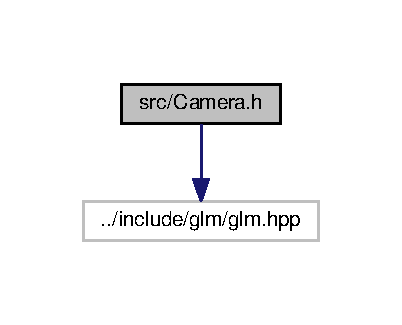
\includegraphics[width=193pt]{_camera_8h__incl}
\end{center}
\end{figure}
This graph shows which files directly or indirectly include this file\+:\nopagebreak
\begin{figure}[H]
\begin{center}
\leavevmode
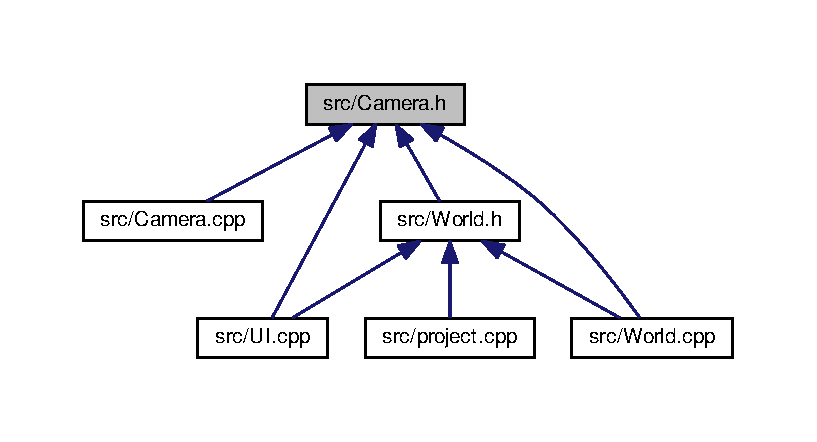
\includegraphics[width=350pt]{_camera_8h__dep__incl}
\end{center}
\end{figure}
\subsection*{Classes}
\begin{DoxyCompactItemize}
\item 
class \hyperlink{class_camera}{Camera}
\end{DoxyCompactItemize}

\hypertarget{glhelper_8cpp}{}\section{src/glhelper.cpp File Reference}
\label{glhelper_8cpp}\index{src/glhelper.\+cpp@{src/glhelper.\+cpp}}
{\ttfamily \#include $<$iostream$>$}\\*
{\ttfamily \#include \char`\"{}../include/glew.\+h\char`\"{}}\\*
{\ttfamily \#include \char`\"{}../include/glfw3.\+h\char`\"{}}\\*
{\ttfamily \#include \char`\"{}glhelper.\+h\char`\"{}}\\*
Include dependency graph for glhelper.\+cpp\+:\nopagebreak
\begin{figure}[H]
\begin{center}
\leavevmode
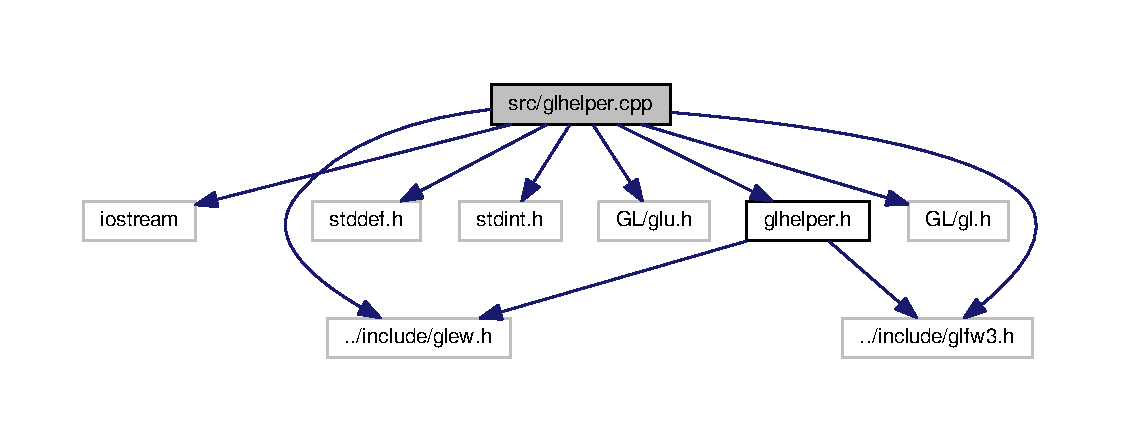
\includegraphics[width=350pt]{glhelper_8cpp__incl}
\end{center}
\end{figure}

\hypertarget{glhelper_8h}{}\section{src/glhelper.h File Reference}
\label{glhelper_8h}\index{src/glhelper.\+h@{src/glhelper.\+h}}
{\ttfamily \#include \char`\"{}../include/glew.\+h\char`\"{}}\\*
{\ttfamily \#include \char`\"{}../include/glfw3.\+h\char`\"{}}\\*
Include dependency graph for glhelper.\+h\+:\nopagebreak
\begin{figure}[H]
\begin{center}
\leavevmode
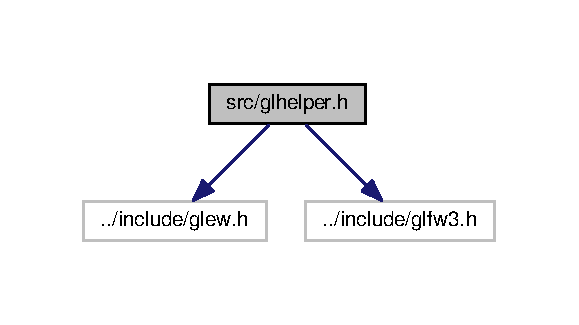
\includegraphics[width=278pt]{glhelper_8h__incl}
\end{center}
\end{figure}
This graph shows which files directly or indirectly include this file\+:\nopagebreak
\begin{figure}[H]
\begin{center}
\leavevmode
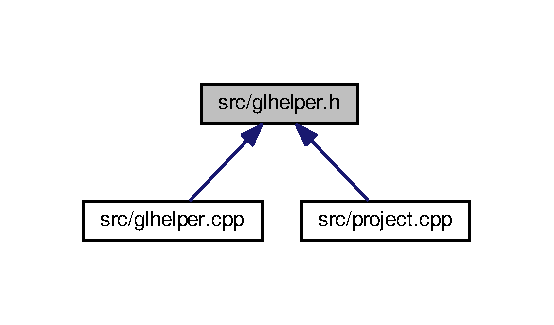
\includegraphics[width=266pt]{glhelper_8h__dep__incl}
\end{center}
\end{figure}
\subsection*{Namespaces}
\begin{DoxyCompactItemize}
\item 
 \hyperlink{namespaceglhelper}{glhelper}
\end{DoxyCompactItemize}
\subsection*{Functions}
\begin{DoxyCompactItemize}
\item 
G\+L\+F\+Wwindow $\ast$ \hyperlink{namespaceglhelper_a85794f1bd977739856a424facd8f5997}{glhelper\+::init\+GL} ()
\item 
void \hyperlink{namespaceglhelper_ad036cebbb4e6d4d91894d7711899e881}{glhelper\+::glfw\+\_\+error\+\_\+callback} (int error, const char $\ast$description)
\end{DoxyCompactItemize}
\subsection*{Variables}
\begin{DoxyCompactItemize}
\item 
const int \hyperlink{namespaceglhelper_ab40d949f334fd21e9fe0f64429f60446}{glhelper\+::\+O\+P\+E\+N\+G\+L\+\_\+\+V\+E\+R\+S\+I\+O\+N\+\_\+\+M\+A\+J\+OR} = 3
\item 
const int \hyperlink{namespaceglhelper_a20bcdbfa51ca5b1ccf42446d6487398f}{glhelper\+::\+O\+P\+E\+N\+G\+L\+\_\+\+V\+E\+R\+S\+I\+O\+N\+\_\+\+M\+I\+N\+OR} = 3
\item 
const G\+Luint \hyperlink{namespaceglhelper_ad10f93be5cc81472c972915bbcb85a82}{glhelper\+::\+W\+I\+N\+D\+O\+W\+\_\+\+W\+I\+D\+TH} = 800
\item 
const G\+Luint \hyperlink{namespaceglhelper_ac85338fb10b2fc3c3efab9639d5c64db}{glhelper\+::\+W\+I\+N\+D\+O\+W\+\_\+\+H\+E\+I\+G\+HT} = 600
\end{DoxyCompactItemize}

\hypertarget{_l_system_8h}{}\section{src/\+L\+System.h File Reference}
\label{_l_system_8h}\index{src/\+L\+System.\+h@{src/\+L\+System.\+h}}
{\ttfamily \#include $<$unordered\+\_\+map$>$}\\*
Include dependency graph for L\+System.\+h\+:\nopagebreak
\begin{figure}[H]
\begin{center}
\leavevmode
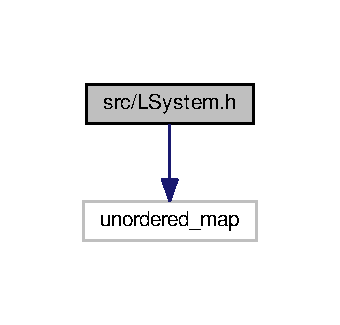
\includegraphics[width=163pt]{_l_system_8h__incl}
\end{center}
\end{figure}
This graph shows which files directly or indirectly include this file\+:\nopagebreak
\begin{figure}[H]
\begin{center}
\leavevmode
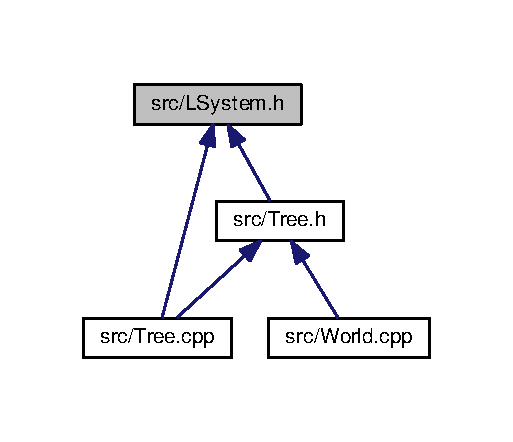
\includegraphics[width=246pt]{_l_system_8h__dep__incl}
\end{center}
\end{figure}
\subsection*{Classes}
\begin{DoxyCompactItemize}
\item 
class \hyperlink{class_l_system}{L\+System$<$ action\+Signature $>$}
\item 
struct \hyperlink{struct_l_system_1_1_rule}{L\+System$<$ action\+Signature $>$\+::\+Rule}
\end{DoxyCompactItemize}

\hypertarget{_material_8cpp}{}\section{src/\+Material.cpp File Reference}
\label{_material_8cpp}\index{src/\+Material.\+cpp@{src/\+Material.\+cpp}}
{\ttfamily \#include \char`\"{}Material.\+h\char`\"{}}\\*
{\ttfamily \#include \char`\"{}../include/glm/gtc/type\+\_\+ptr.\+hpp\char`\"{}}\\*
Include dependency graph for Material.\+cpp\+:\nopagebreak
\begin{figure}[H]
\begin{center}
\leavevmode
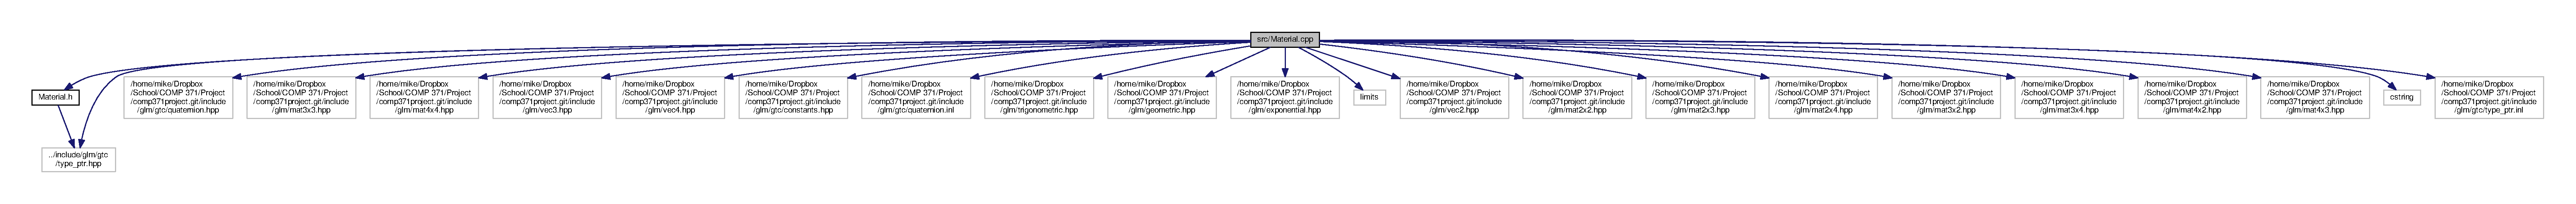
\includegraphics[width=350pt]{_material_8cpp__incl}
\end{center}
\end{figure}
\subsection*{Namespaces}
\begin{DoxyCompactItemize}
\item 
 \hyperlink{namespace_materials}{Materials}
\end{DoxyCompactItemize}
\subsection*{Variables}
\begin{DoxyCompactItemize}
\item 
\hyperlink{struct_material}{Material} \hyperlink{namespace_materials_adb662ea7a8869f3cba2dcf125ac0d902}{Materials\+::brass}
\item 
\hyperlink{struct_material}{Material} \hyperlink{namespace_materials_aef75c359633b069fb948443f8011afb1}{Materials\+::bronze}
\item 
\hyperlink{struct_material}{Material} \hyperlink{namespace_materials_a74ca93b9b8f4b91eac56e29dcf2f4fb4}{Materials\+::polished\+Bronze}
\item 
\hyperlink{struct_material}{Material} \hyperlink{namespace_materials_ae1d90d5c8c231d887fd22e459a4632ca}{Materials\+::chrome}
\item 
\hyperlink{struct_material}{Material} \hyperlink{namespace_materials_a00e102c39a09ca4fd6932f43094af174}{Materials\+::copper}
\item 
\hyperlink{struct_material}{Material} \hyperlink{namespace_materials_a2140516cc8e291d497ac00dbd73d8fbd}{Materials\+::polished\+Copper}
\item 
\hyperlink{struct_material}{Material} \hyperlink{namespace_materials_aaa1f200530d72d7ee11f5fc492f82bf9}{Materials\+::gold}
\item 
\hyperlink{struct_material}{Material} \hyperlink{namespace_materials_a714fa575786b960faa0e02dac82a4435}{Materials\+::polished\+Gold}
\item 
\hyperlink{struct_material}{Material} \hyperlink{namespace_materials_a125b4c95ab2ef64d802378762572abea}{Materials\+::pewter}
\item 
\hyperlink{struct_material}{Material} \hyperlink{namespace_materials_a566238bc6d1fe2f5e8a78e2031b8eb09}{Materials\+::silver}
\item 
\hyperlink{struct_material}{Material} \hyperlink{namespace_materials_aca88f7adaadc3a3bbfce3dea0c276451}{Materials\+::polished\+Silver}
\item 
\hyperlink{struct_material}{Material} \hyperlink{namespace_materials_af0d20fbbd84514c88dc37f22beb5ff8e}{Materials\+::emerald}
\item 
\hyperlink{struct_material}{Material} \hyperlink{namespace_materials_a5fc7c043507c2cea752070b593ca85aa}{Materials\+::jade}
\item 
\hyperlink{struct_material}{Material} \hyperlink{namespace_materials_ac8f37f7d2fdb484dee3ceab10190ba5f}{Materials\+::obsidian}
\item 
\hyperlink{struct_material}{Material} \hyperlink{namespace_materials_a3b1f30a53ed581645b32a371a3f18518}{Materials\+::pearl}
\item 
\hyperlink{struct_material}{Material} \hyperlink{namespace_materials_a0440cdfea64816f17c8616a5bbf626e2}{Materials\+::ruby}
\item 
\hyperlink{struct_material}{Material} \hyperlink{namespace_materials_ab5b494a26565e795963d6b448cb62516}{Materials\+::turquoise}
\item 
\hyperlink{struct_material}{Material} \hyperlink{namespace_materials_a8676bb061fa114ca6cde5b899d1d6b71}{Materials\+::black\+Plastic}
\item 
\hyperlink{struct_material}{Material} \hyperlink{namespace_materials_af18248a1ab616cf0a0c3cc026a3a7231}{Materials\+::black\+Rubber}
\end{DoxyCompactItemize}

\hypertarget{_material_8h}{}\section{src/\+Material.h File Reference}
\label{_material_8h}\index{src/\+Material.\+h@{src/\+Material.\+h}}
{\ttfamily \#include \char`\"{}../include/glm/gtc/type\+\_\+ptr.\+hpp\char`\"{}}\\*
Include dependency graph for Material.\+h\+:\nopagebreak
\begin{figure}[H]
\begin{center}
\leavevmode
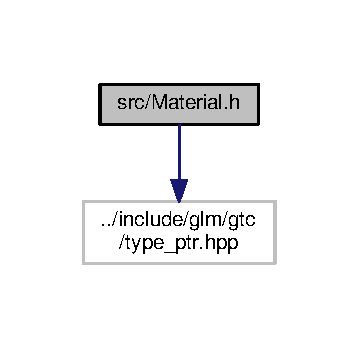
\includegraphics[width=172pt]{_material_8h__incl}
\end{center}
\end{figure}
This graph shows which files directly or indirectly include this file\+:
\nopagebreak
\begin{figure}[H]
\begin{center}
\leavevmode
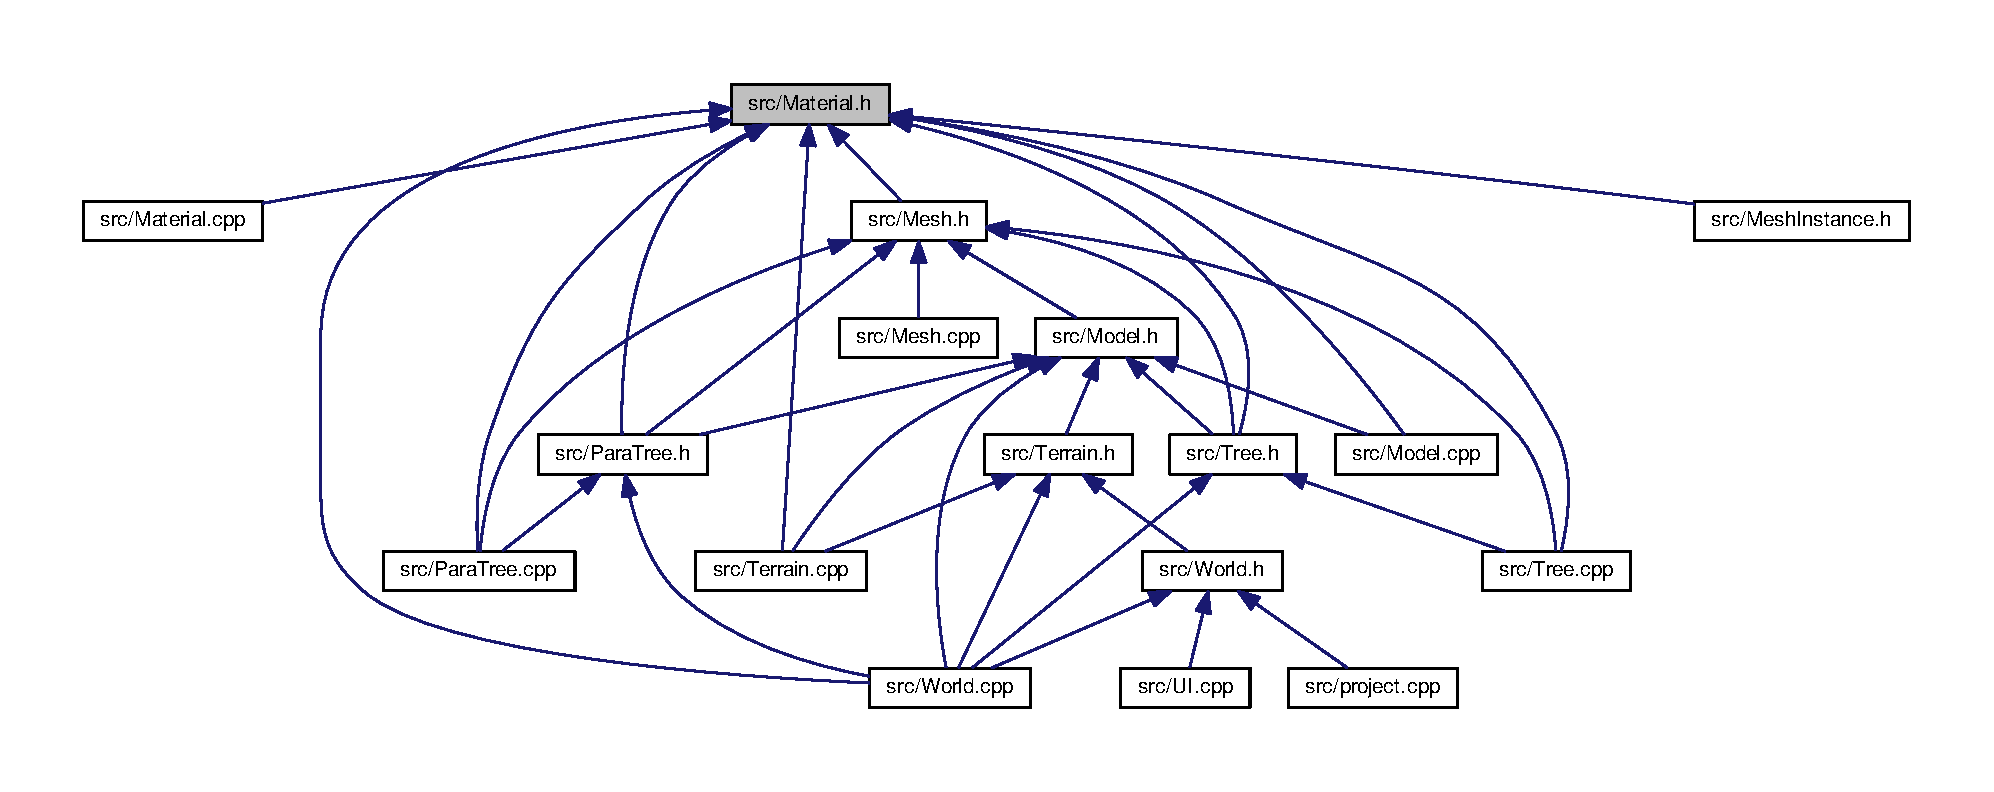
\includegraphics[width=350pt]{_material_8h__dep__incl}
\end{center}
\end{figure}
\subsection*{Classes}
\begin{DoxyCompactItemize}
\item 
struct \hyperlink{struct_material}{Material}
\end{DoxyCompactItemize}
\subsection*{Namespaces}
\begin{DoxyCompactItemize}
\item 
 \hyperlink{namespace_materials}{Materials}
\end{DoxyCompactItemize}

\hypertarget{_mesh_8cpp}{}\section{src/\+Mesh.cpp File Reference}
\label{_mesh_8cpp}\index{src/\+Mesh.\+cpp@{src/\+Mesh.\+cpp}}
{\ttfamily \#include $<$vector$>$}\\*
{\ttfamily \#include $<$string$>$}\\*
{\ttfamily \#include $<$algorithm$>$}\\*
{\ttfamily \#include \char`\"{}../include/glew.\+h\char`\"{}}\\*
{\ttfamily \#include \char`\"{}../include/glfw3.\+h\char`\"{}}\\*
{\ttfamily \#include \char`\"{}../include/glm/gtc/type\+\_\+ptr.\+hpp\char`\"{}}\\*
{\ttfamily \#include \char`\"{}Shader.\+h\char`\"{}}\\*
{\ttfamily \#include \char`\"{}Mesh.\+h\char`\"{}}\\*
{\ttfamily \#include $<$iostream$>$}\\*
Include dependency graph for Mesh.\+cpp\+:\nopagebreak
\begin{figure}[H]
\begin{center}
\leavevmode

\includegraphics[width=350pt]{_mesh_8cpp__incl}
\end{center}
\end{figure}

\hypertarget{_mesh_8h}{}\section{src/\+Mesh.h File Reference}
\label{_mesh_8h}\index{src/\+Mesh.\+h@{src/\+Mesh.\+h}}
{\ttfamily \#include $<$vector$>$}\\*
{\ttfamily \#include $<$string$>$}\\*
{\ttfamily \#include \char`\"{}../include/glew.\+h\char`\"{}}\\*
{\ttfamily \#include \char`\"{}../include/glfw3.\+h\char`\"{}}\\*
{\ttfamily \#include \char`\"{}../include/glm/gtc/type\+\_\+ptr.\+hpp\char`\"{}}\\*
{\ttfamily \#include \char`\"{}../include/glm/gtc/matrix\+\_\+transform.\+hpp\char`\"{}}\\*
{\ttfamily \#include \char`\"{}Vertex.\+h\char`\"{}}\\*
{\ttfamily \#include \char`\"{}Shader.\+h\char`\"{}}\\*
{\ttfamily \#include \char`\"{}Material.\+h\char`\"{}}\\*
{\ttfamily \#include $<$iostream$>$}\\*
{\ttfamily \#include \char`\"{}../include/glm/gtx/string\+\_\+cast.\+hpp\char`\"{}}\\*
Include dependency graph for Mesh.\+h\+:\nopagebreak
\begin{figure}[H]
\begin{center}
\leavevmode
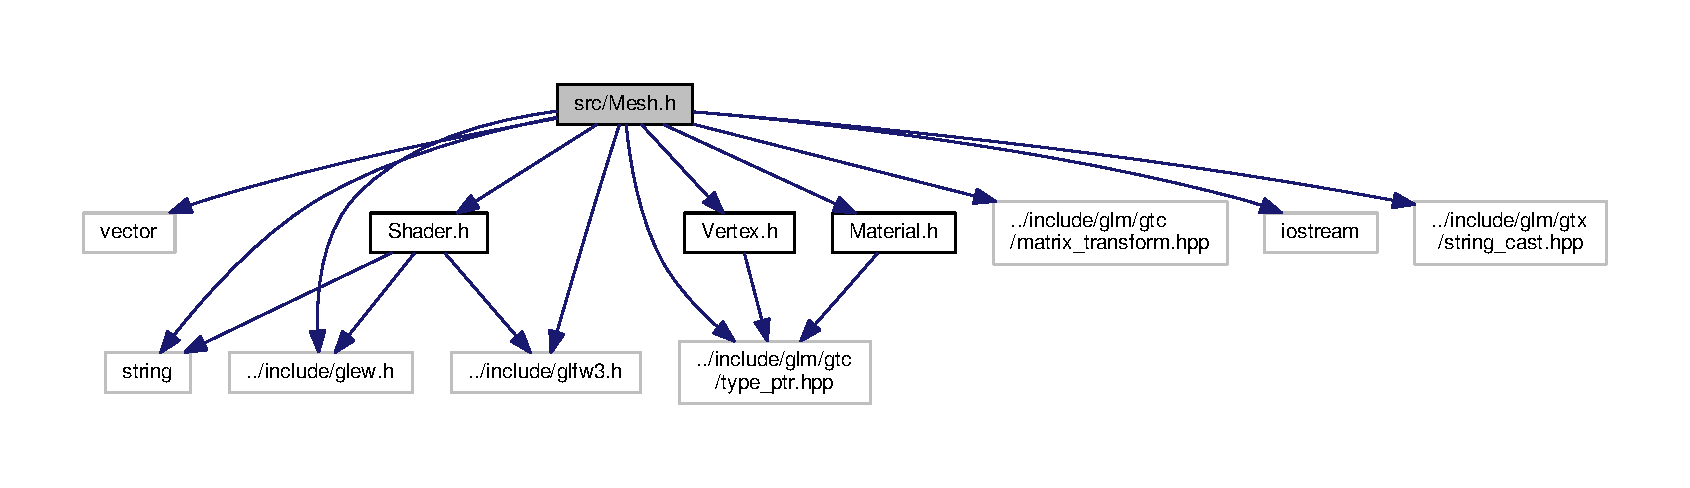
\includegraphics[width=350pt]{_mesh_8h__incl}
\end{center}
\end{figure}
This graph shows which files directly or indirectly include this file\+:
\nopagebreak
\begin{figure}[H]
\begin{center}
\leavevmode
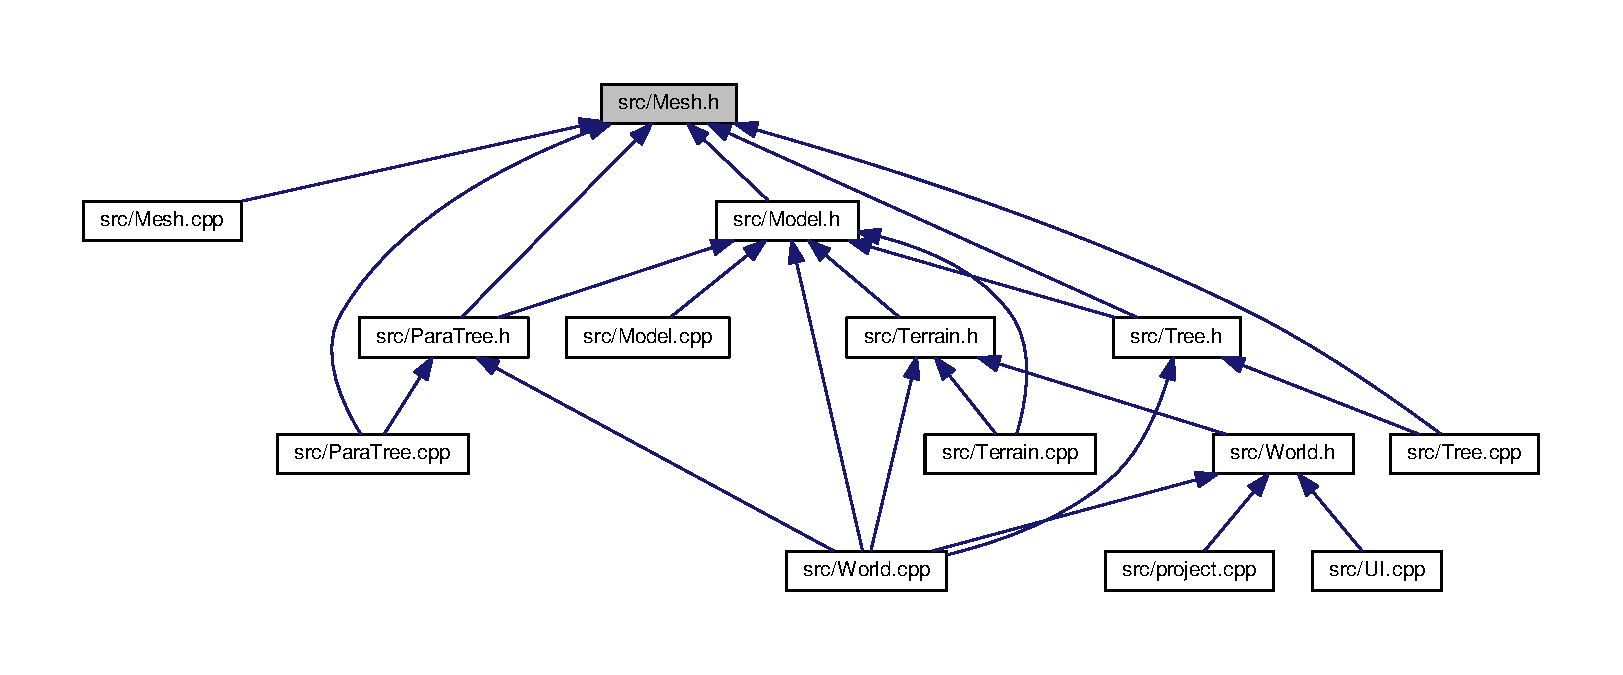
\includegraphics[width=350pt]{_mesh_8h__dep__incl}
\end{center}
\end{figure}
\subsection*{Classes}
\begin{DoxyCompactItemize}
\item 
class \hyperlink{class_mesh}{Mesh}
\item 
class \hyperlink{class_mesh_instance_ptr}{Mesh\+Instance\+Ptr}
\item 
class \hyperlink{class_mesh_instance}{Mesh\+Instance}
\end{DoxyCompactItemize}

\hypertarget{_mesh_instance_8h}{}\section{src/\+Mesh\+Instance.h File Reference}
\label{_mesh_instance_8h}\index{src/\+Mesh\+Instance.\+h@{src/\+Mesh\+Instance.\+h}}
{\ttfamily \#include $<$vector$>$}\\*
{\ttfamily \#include \char`\"{}../include/glm/gtc/type\+\_\+ptr.\+hpp\char`\"{}}\\*
{\ttfamily \#include \char`\"{}Material.\+h\char`\"{}}\\*
Include dependency graph for Mesh\+Instance.\+h\+:\nopagebreak
\begin{figure}[H]
\begin{center}
\leavevmode
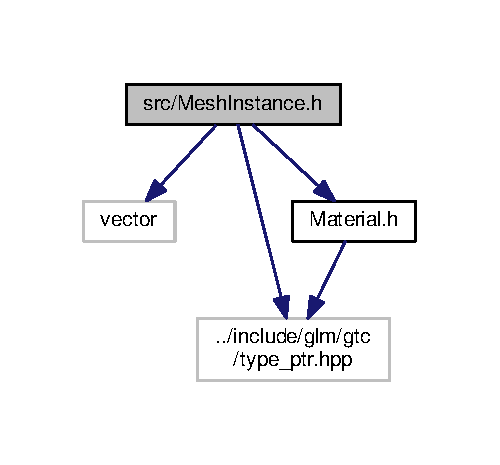
\includegraphics[width=240pt]{_mesh_instance_8h__incl}
\end{center}
\end{figure}
\subsection*{Classes}
\begin{DoxyCompactItemize}
\item 
class \hyperlink{class_mesh_instance}{Mesh\+Instance}
\end{DoxyCompactItemize}

\hypertarget{_model_8cpp}{}\section{src/\+Model.cpp File Reference}
\label{_model_8cpp}\index{src/\+Model.\+cpp@{src/\+Model.\+cpp}}
{\ttfamily \#include \char`\"{}../include/glew.\+h\char`\"{}}\\*
{\ttfamily \#include \char`\"{}../include/glfw3.\+h\char`\"{}}\\*
{\ttfamily \#include \char`\"{}../include/glm/gtc/type\+\_\+ptr.\+hpp\char`\"{}}\\*
{\ttfamily \#include \char`\"{}../include/glm/gtc/matrix\+\_\+transform.\+hpp\char`\"{}}\\*
{\ttfamily \#include $<$vector$>$}\\*
{\ttfamily \#include \char`\"{}Shader.\+h\char`\"{}}\\*
{\ttfamily \#include \char`\"{}Material.\+h\char`\"{}}\\*
{\ttfamily \#include \char`\"{}Model.\+h\char`\"{}}\\*
Include dependency graph for Model.\+cpp\+:\nopagebreak
\begin{figure}[H]
\begin{center}
\leavevmode
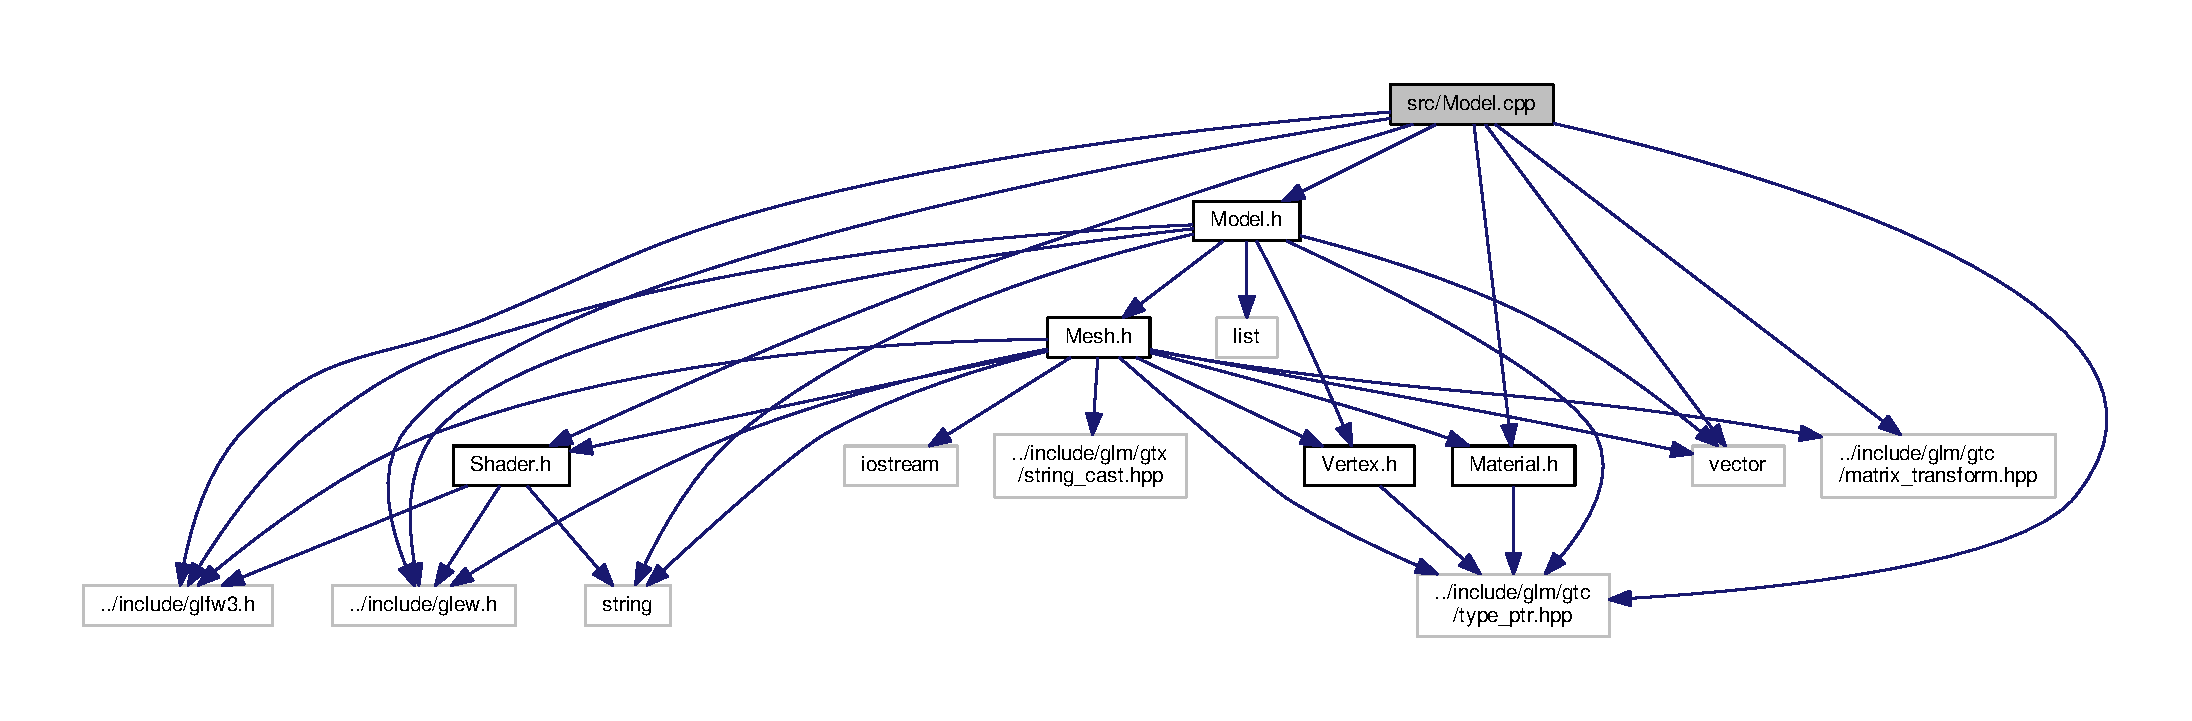
\includegraphics[width=350pt]{_model_8cpp__incl}
\end{center}
\end{figure}

\hypertarget{_model_8h}{}\section{src/\+Model.h File Reference}
\label{_model_8h}\index{src/\+Model.\+h@{src/\+Model.\+h}}
{\ttfamily \#include $<$vector$>$}\\*
{\ttfamily \#include $<$list$>$}\\*
{\ttfamily \#include $<$string$>$}\\*
{\ttfamily \#include \char`\"{}../include/glew.\+h\char`\"{}}\\*
{\ttfamily \#include \char`\"{}../include/glfw3.\+h\char`\"{}}\\*
{\ttfamily \#include \char`\"{}../include/glm/gtc/type\+\_\+ptr.\+hpp\char`\"{}}\\*
{\ttfamily \#include \char`\"{}Vertex.\+h\char`\"{}}\\*
{\ttfamily \#include \char`\"{}Mesh.\+h\char`\"{}}\\*
Include dependency graph for Model.\+h\+:\nopagebreak
\begin{figure}[H]
\begin{center}
\leavevmode
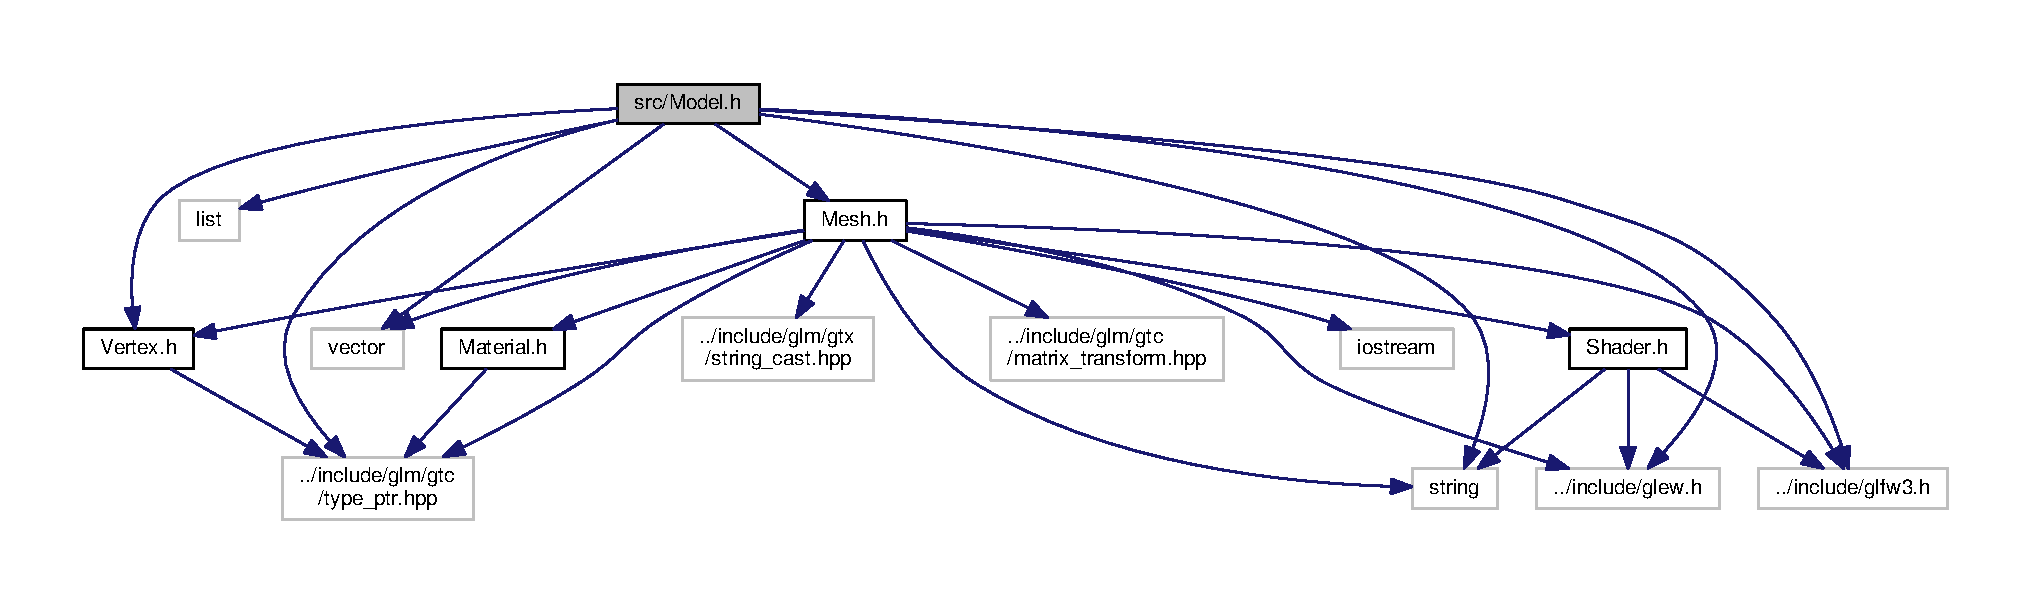
\includegraphics[width=350pt]{_model_8h__incl}
\end{center}
\end{figure}
This graph shows which files directly or indirectly include this file\+:\nopagebreak
\begin{figure}[H]
\begin{center}
\leavevmode
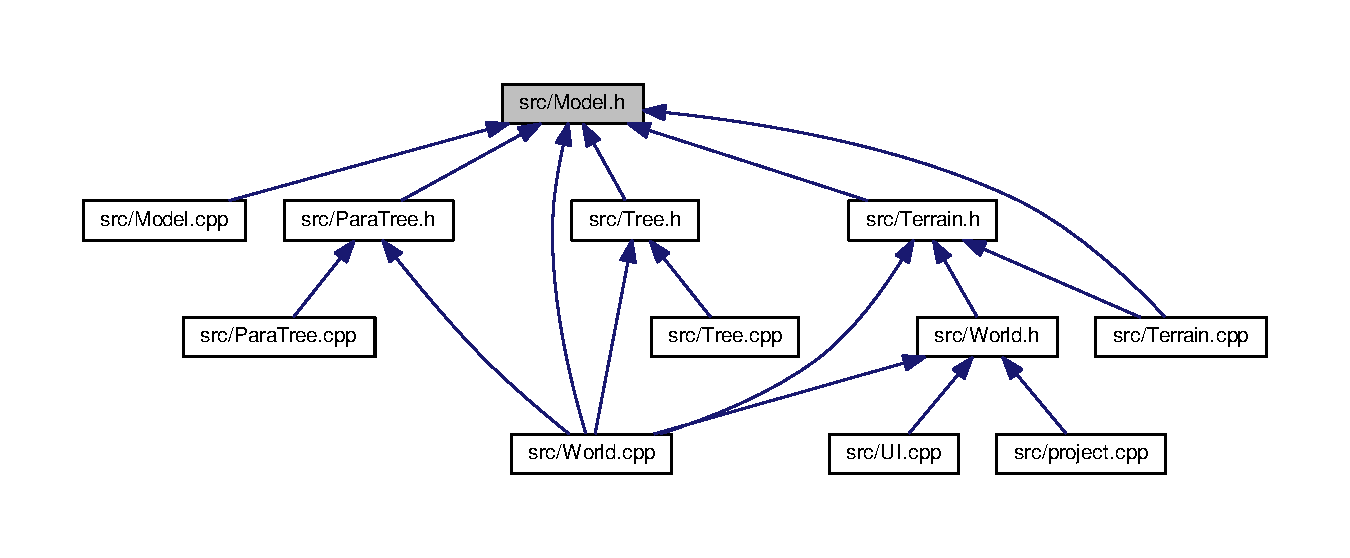
\includegraphics[width=350pt]{_model_8h__dep__incl}
\end{center}
\end{figure}
\subsection*{Classes}
\begin{DoxyCompactItemize}
\item 
class \hyperlink{class_model}{Model}
\end{DoxyCompactItemize}

\hypertarget{_para_tree_8cpp}{}\section{src/\+Para\+Tree.cpp File Reference}
\label{_para_tree_8cpp}\index{src/\+Para\+Tree.\+cpp@{src/\+Para\+Tree.\+cpp}}
{\ttfamily \#include \char`\"{}Para\+Tree.\+h\char`\"{}}\\*
{\ttfamily \#include $<$string$>$}\\*
{\ttfamily \#include $<$cstring$>$}\\*
{\ttfamily \#include $<$algorithm$>$}\\*
{\ttfamily \#include $<$unordered\+\_\+map$>$}\\*
{\ttfamily \#include $<$vector$>$}\\*
{\ttfamily \#include $<$list$>$}\\*
{\ttfamily \#include $<$functional$>$}\\*
{\ttfamily \#include \char`\"{}../include/glm/gtc/type\+\_\+ptr.\+hpp\char`\"{}}\\*
{\ttfamily \#include \char`\"{}Vertex.\+h\char`\"{}}\\*
{\ttfamily \#include \char`\"{}Mesh.\+h\char`\"{}}\\*
{\ttfamily \#include \char`\"{}Shader.\+h\char`\"{}}\\*
{\ttfamily \#include \char`\"{}Material.\+h\char`\"{}}\\*
{\ttfamily \#include \char`\"{}P\+L\+S.\+h\char`\"{}}\\*
{\ttfamily \#include \char`\"{}Turtle.\+h\char`\"{}}\\*
{\ttfamily \#include $<$stdio.\+h$>$}\\*
{\ttfamily \#include $<$iostream$>$}\\*
{\ttfamily \#include \char`\"{}../include/glm/gtx/string\+\_\+cast.\+hpp\char`\"{}}\\*
Include dependency graph for Para\+Tree.\+cpp\+:\nopagebreak
\begin{figure}[H]
\begin{center}
\leavevmode
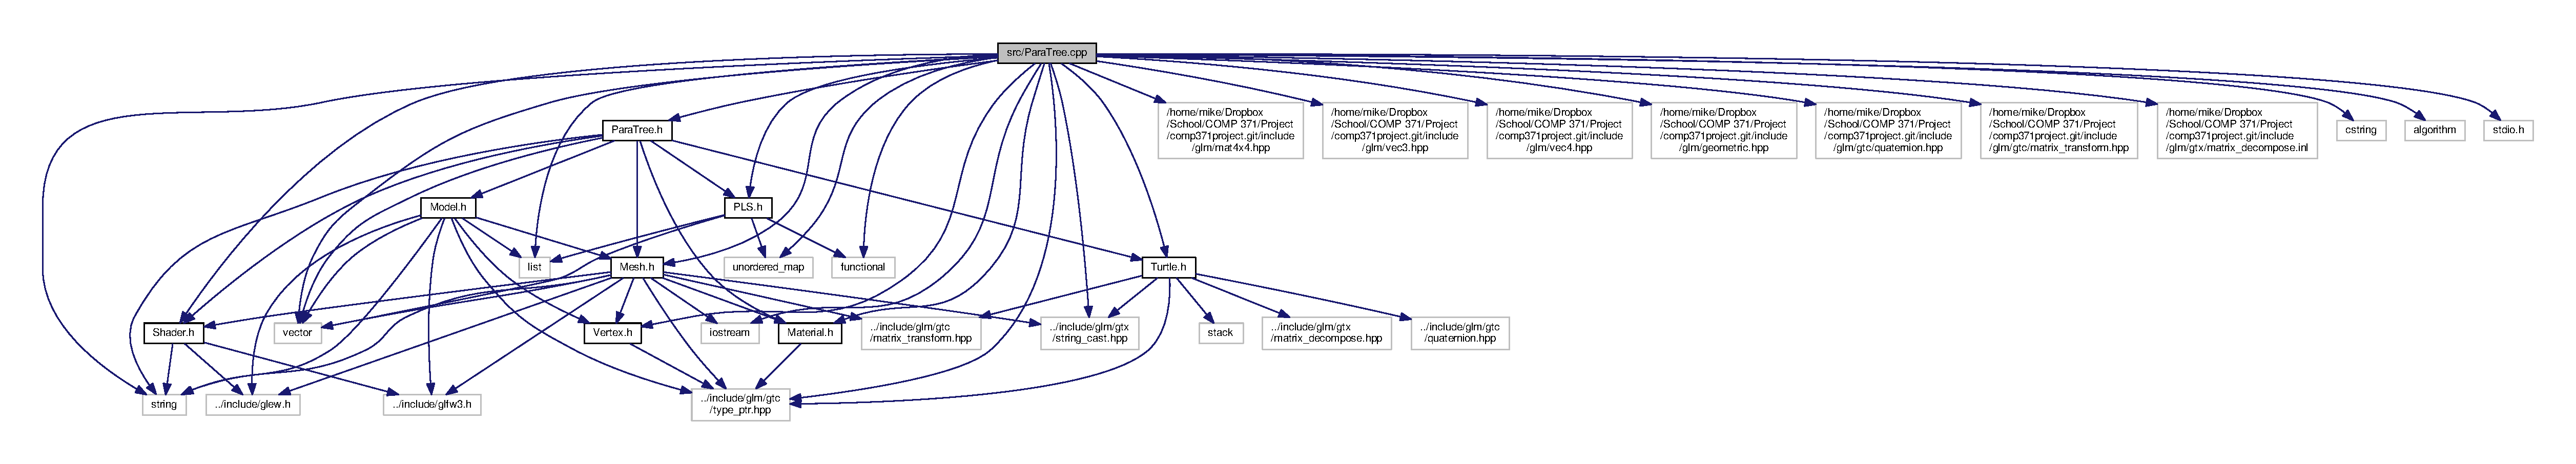
\includegraphics[width=350pt]{_para_tree_8cpp__incl}
\end{center}
\end{figure}

\hypertarget{_para_tree_8h}{}\section{src/\+Para\+Tree.h File Reference}
\label{_para_tree_8h}\index{src/\+Para\+Tree.\+h@{src/\+Para\+Tree.\+h}}
{\ttfamily \#include $<$vector$>$}\\*
{\ttfamily \#include $<$string$>$}\\*
{\ttfamily \#include \char`\"{}Shader.\+h\char`\"{}}\\*
{\ttfamily \#include \char`\"{}Material.\+h\char`\"{}}\\*
{\ttfamily \#include \char`\"{}Mesh.\+h\char`\"{}}\\*
{\ttfamily \#include \char`\"{}Model.\+h\char`\"{}}\\*
{\ttfamily \#include \char`\"{}P\+L\+S.\+h\char`\"{}}\\*
{\ttfamily \#include \char`\"{}Turtle.\+h\char`\"{}}\\*
Include dependency graph for Para\+Tree.\+h\+:\nopagebreak
\begin{figure}[H]
\begin{center}
\leavevmode
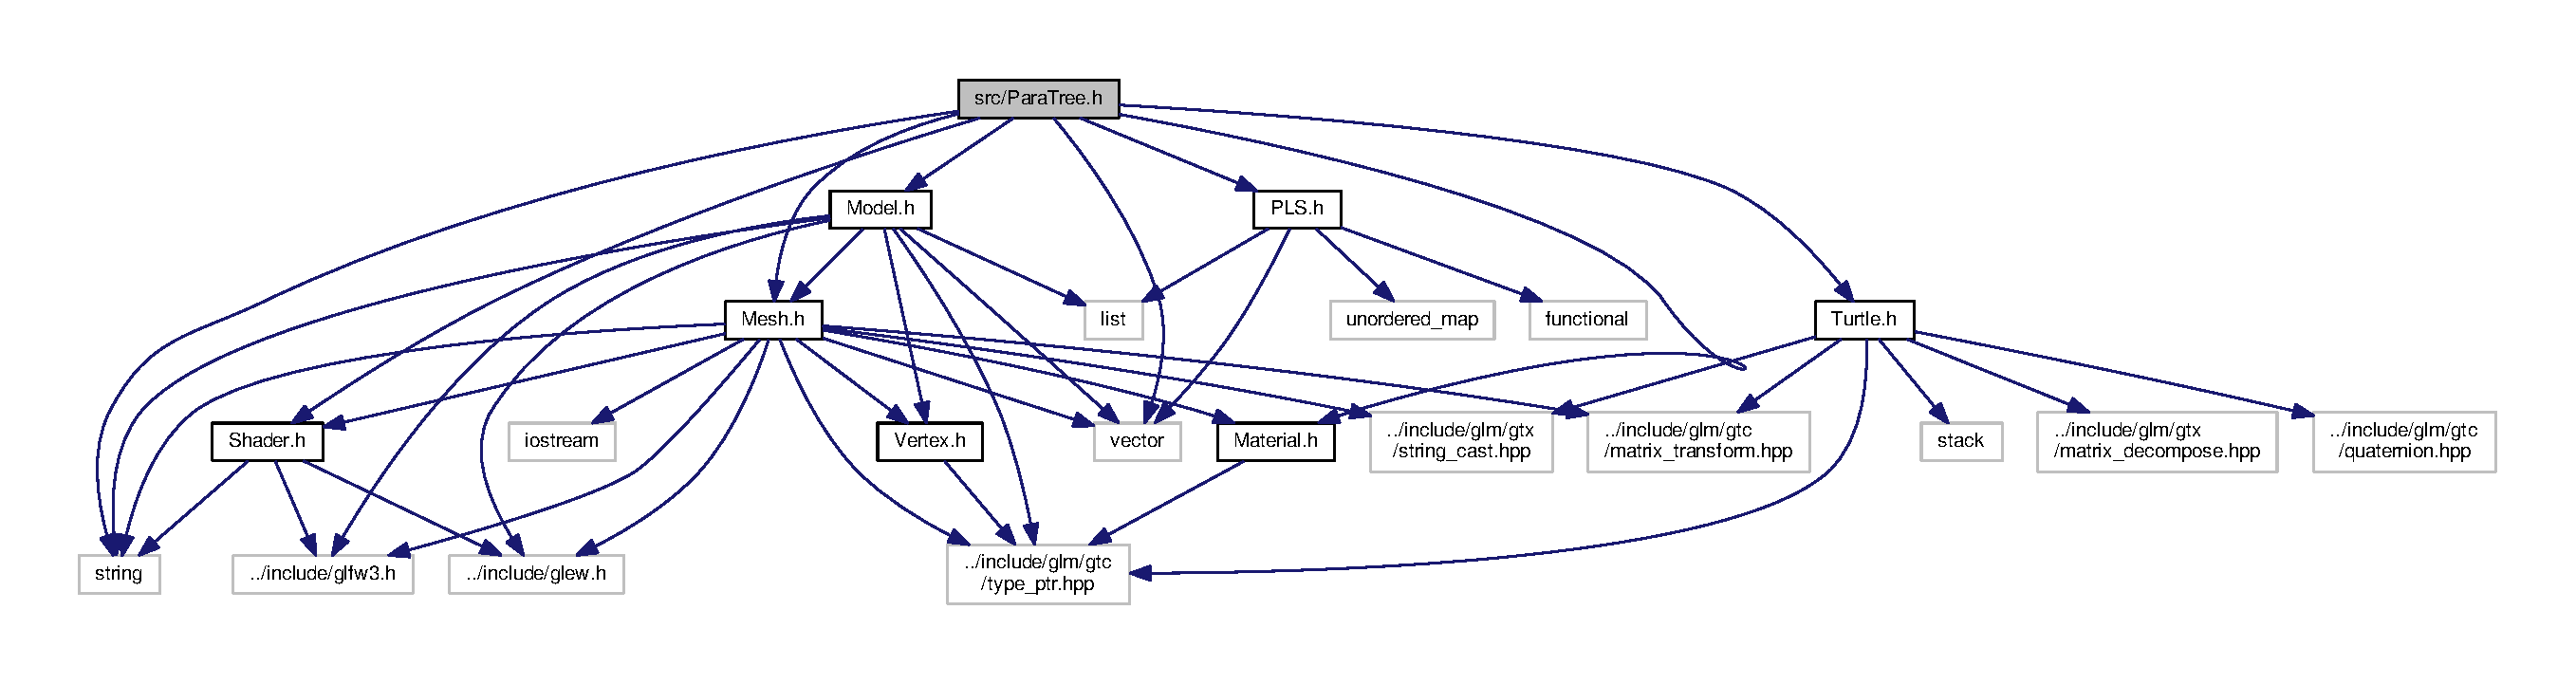
\includegraphics[width=350pt]{_para_tree_8h__incl}
\end{center}
\end{figure}
This graph shows which files directly or indirectly include this file\+:\nopagebreak
\begin{figure}[H]
\begin{center}
\leavevmode
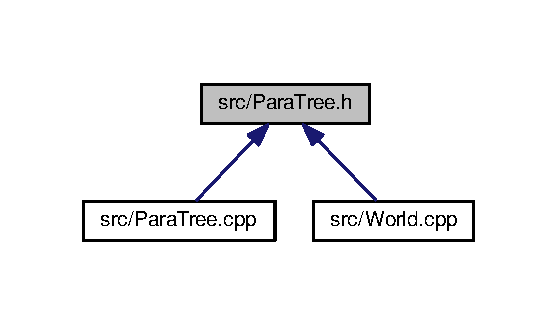
\includegraphics[width=268pt]{_para_tree_8h__dep__incl}
\end{center}
\end{figure}
\subsection*{Classes}
\begin{DoxyCompactItemize}
\item 
class \hyperlink{class_para_tree}{Para\+Tree}
\item 
struct \hyperlink{struct_para_tree_1_1_tree_params}{Para\+Tree\+::\+Tree\+Params}
\item 
struct \hyperlink{struct_para_tree_1_1_presets}{Para\+Tree\+::\+Presets}
\item 
struct \hyperlink{struct_para_tree_1_1_actions}{Para\+Tree\+::\+Actions}
\end{DoxyCompactItemize}

\hypertarget{_p_l_s_8h}{}\section{src/\+P\+LS.h File Reference}
\label{_p_l_s_8h}\index{src/\+P\+L\+S.\+h@{src/\+P\+L\+S.\+h}}
{\ttfamily \#include $<$unordered\+\_\+map$>$}\\*
{\ttfamily \#include $<$vector$>$}\\*
{\ttfamily \#include $<$list$>$}\\*
{\ttfamily \#include $<$functional$>$}\\*
Include dependency graph for P\+L\+S.\+h\+:\nopagebreak
\begin{figure}[H]
\begin{center}
\leavevmode
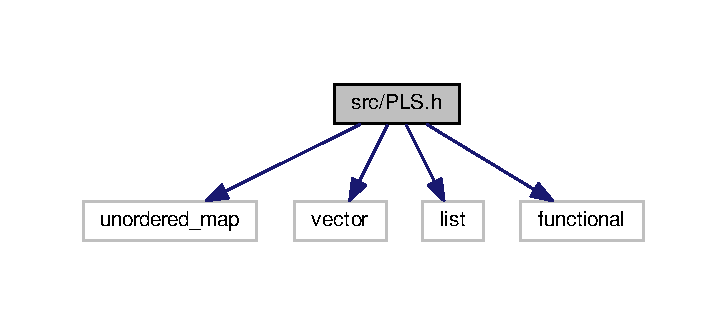
\includegraphics[width=349pt]{_p_l_s_8h__incl}
\end{center}
\end{figure}
This graph shows which files directly or indirectly include this file\+:\nopagebreak
\begin{figure}[H]
\begin{center}
\leavevmode
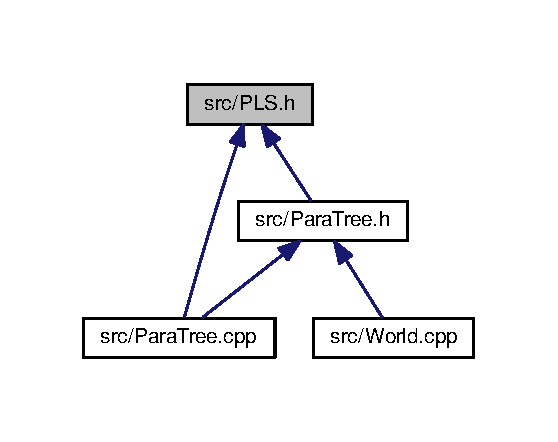
\includegraphics[width=268pt]{_p_l_s_8h__dep__incl}
\end{center}
\end{figure}
\subsection*{Classes}
\begin{DoxyCompactItemize}
\item 
class \hyperlink{class_p_l_s}{P\+LS}
\item 
class \hyperlink{class_p_l_s_1_1_param}{P\+L\+S\+::\+Param}
\item 
class \hyperlink{class_p_l_s_1_1_module}{P\+L\+S\+::\+Module}
\item 
class \hyperlink{class_p_l_s_1_1_production}{P\+L\+S\+::\+Production}
\end{DoxyCompactItemize}

\hypertarget{project_8cpp}{}\section{src/project.cpp File Reference}
\label{project_8cpp}\index{src/project.\+cpp@{src/project.\+cpp}}
{\ttfamily \#include \char`\"{}../include/glew.\+h\char`\"{}}\\*
{\ttfamily \#include \char`\"{}../include/glfw3.\+h\char`\"{}}\\*
{\ttfamily \#include $<$iostream$>$}\\*
{\ttfamily \#include $<$string$>$}\\*
{\ttfamily \#include \char`\"{}glhelper.\+h\char`\"{}}\\*
{\ttfamily \#include \char`\"{}World.\+h\char`\"{}}\\*
{\ttfamily \#include \char`\"{}U\+I.\+h\char`\"{}}\\*
Include dependency graph for project.\+cpp\+:\nopagebreak
\begin{figure}[H]
\begin{center}
\leavevmode
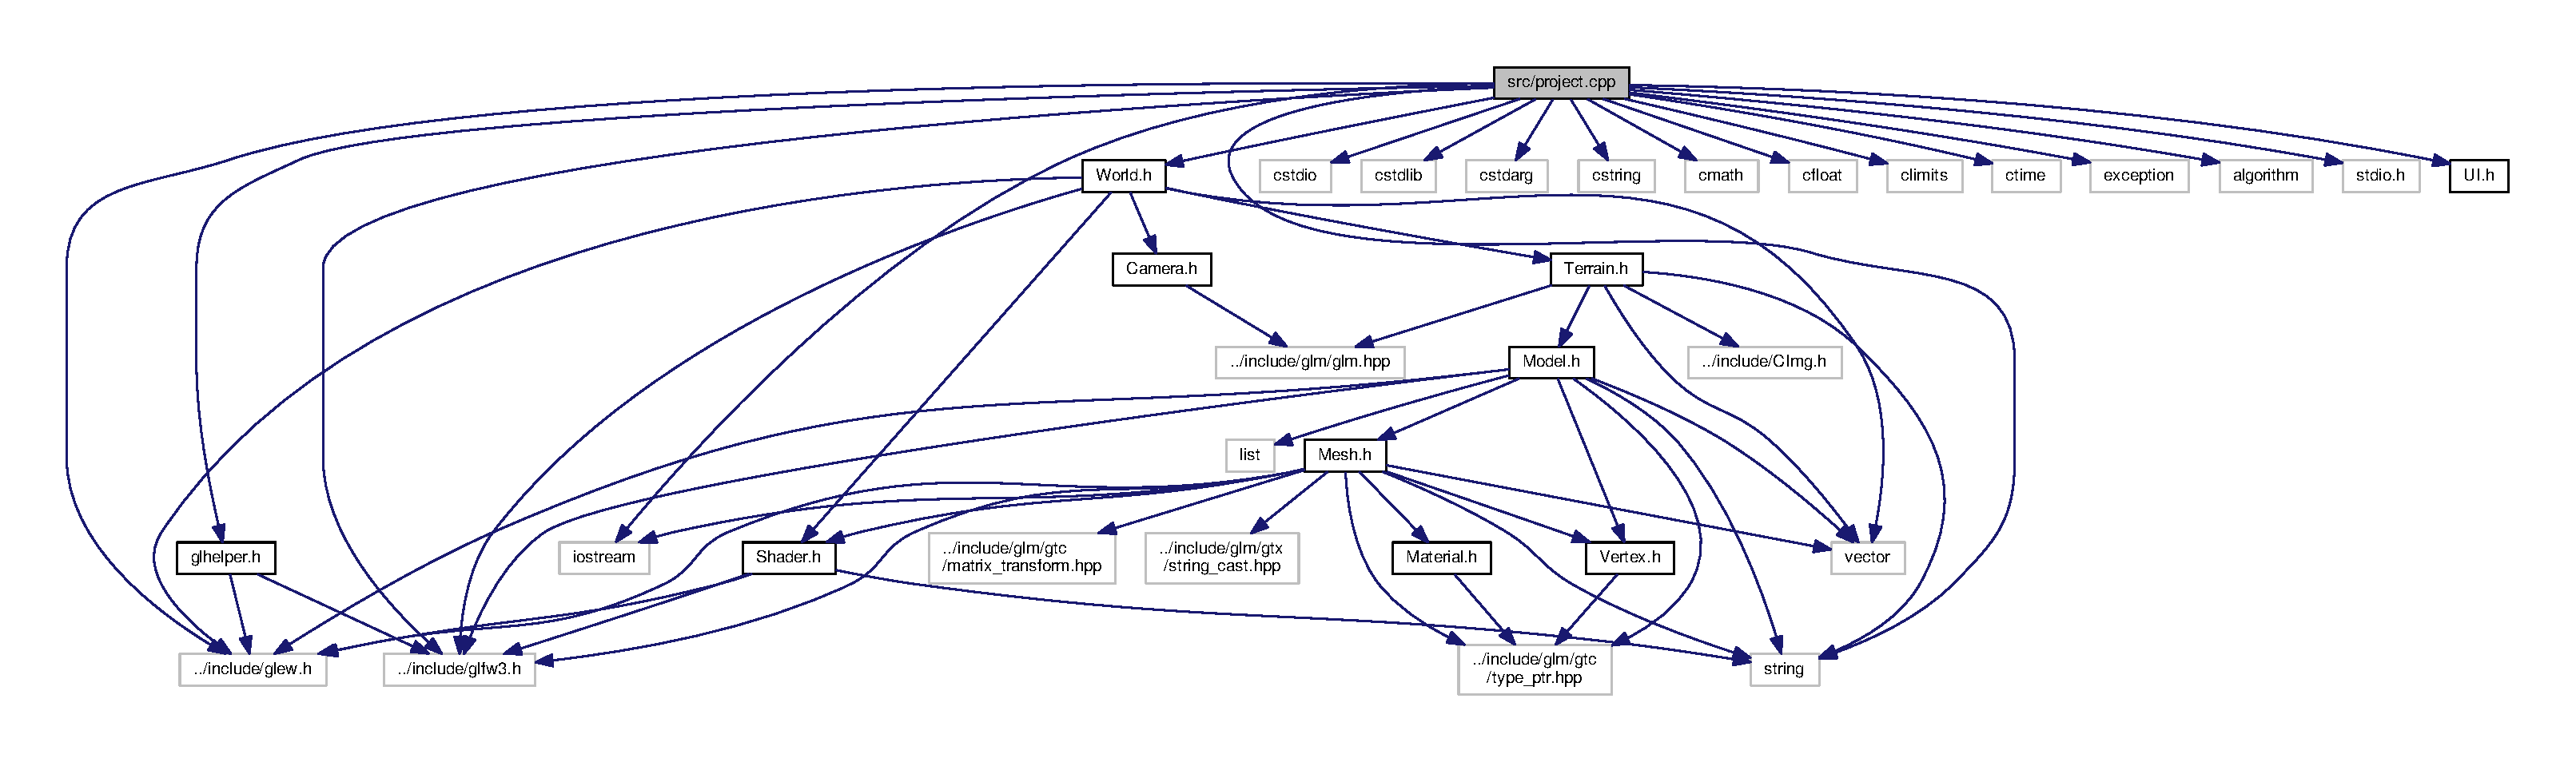
\includegraphics[width=350pt]{project_8cpp__incl}
\end{center}
\end{figure}
\subsection*{Functions}
\begin{DoxyCompactItemize}
\item 
int \hyperlink{project_8cpp_ae66f6b31b5ad750f1fe042a706a4e3d4}{main} ()
\end{DoxyCompactItemize}


\subsection{Function Documentation}
\index{project.\+cpp@{project.\+cpp}!main@{main}}
\index{main@{main}!project.\+cpp@{project.\+cpp}}
\subsubsection[{\texorpdfstring{main()}{main()}}]{\setlength{\rightskip}{0pt plus 5cm}int main (
\begin{DoxyParamCaption}
{}
\end{DoxyParamCaption}
)}\hypertarget{project_8cpp_ae66f6b31b5ad750f1fe042a706a4e3d4}{}\label{project_8cpp_ae66f6b31b5ad750f1fe042a706a4e3d4}

\hypertarget{_shader_8cpp}{}\section{src/\+Shader.cpp File Reference}
\label{_shader_8cpp}\index{src/\+Shader.\+cpp@{src/\+Shader.\+cpp}}
{\ttfamily \#include \char`\"{}../include/glew.\+h\char`\"{}}\\*
{\ttfamily \#include \char`\"{}../include/glfw3.\+h\char`\"{}}\\*
{\ttfamily \#include $<$string$>$}\\*
{\ttfamily \#include $<$fstream$>$}\\*
{\ttfamily \#include \char`\"{}Shader.\+h\char`\"{}}\\*
{\ttfamily \#include $<$iostream$>$}\\*
Include dependency graph for Shader.\+cpp\+:\nopagebreak
\begin{figure}[H]
\begin{center}
\leavevmode
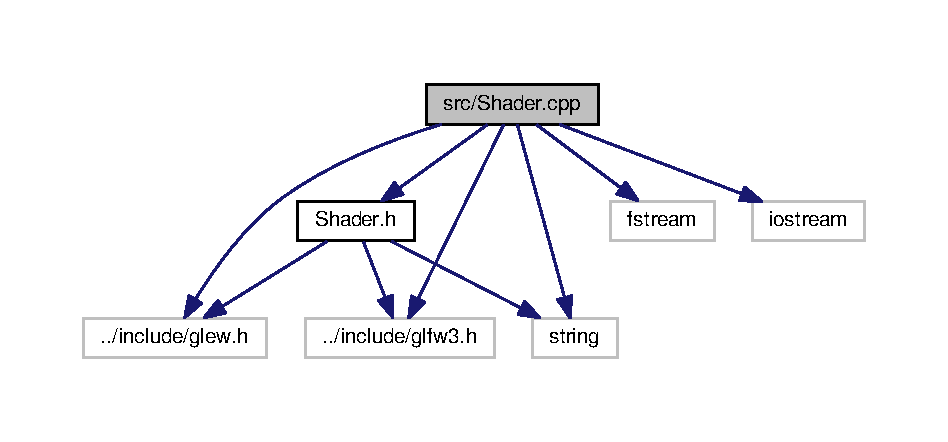
\includegraphics[width=350pt]{_shader_8cpp__incl}
\end{center}
\end{figure}

\hypertarget{_shader_8h}{}\section{src/\+Shader.h File Reference}
\label{_shader_8h}\index{src/\+Shader.\+h@{src/\+Shader.\+h}}
{\ttfamily \#include $<$string$>$}\\*
{\ttfamily \#include \char`\"{}../include/glew.\+h\char`\"{}}\\*
{\ttfamily \#include \char`\"{}../include/glfw3.\+h\char`\"{}}\\*
Include dependency graph for Shader.\+h\+:\nopagebreak
\begin{figure}[H]
\begin{center}
\leavevmode
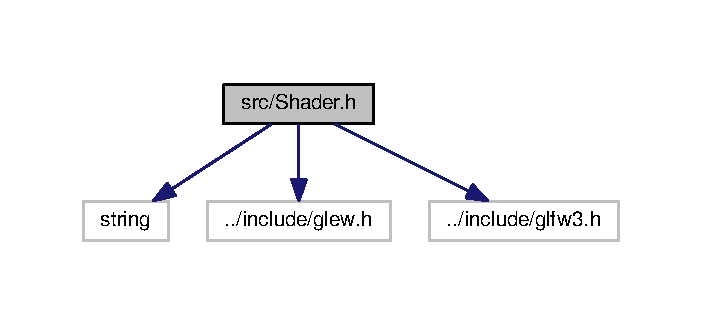
\includegraphics[width=337pt]{_shader_8h__incl}
\end{center}
\end{figure}
This graph shows which files directly or indirectly include this file\+:
\nopagebreak
\begin{figure}[H]
\begin{center}
\leavevmode
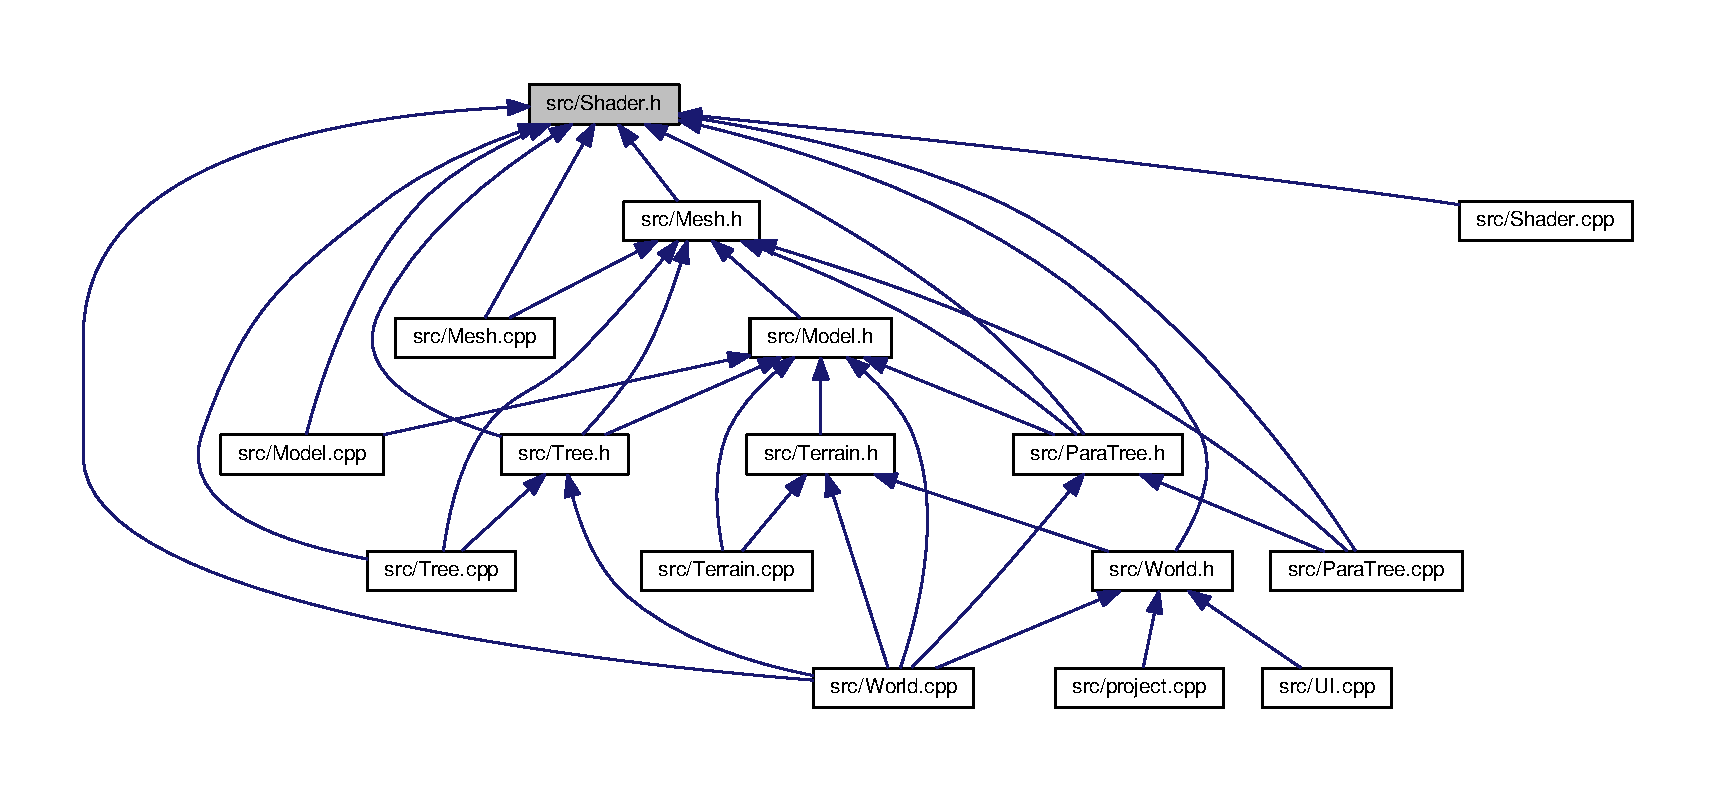
\includegraphics[width=350pt]{_shader_8h__dep__incl}
\end{center}
\end{figure}
\subsection*{Classes}
\begin{DoxyCompactItemize}
\item 
class \hyperlink{class_shader}{Shader}
\end{DoxyCompactItemize}

\hypertarget{_terrain_8cpp}{}\section{src/\+Terrain.cpp File Reference}
\label{_terrain_8cpp}\index{src/\+Terrain.\+cpp@{src/\+Terrain.\+cpp}}
{\ttfamily \#include \char`\"{}../include/glew.\+h\char`\"{}}\\*
{\ttfamily \#include \char`\"{}../include/glfw3.\+h\char`\"{}}\\*
{\ttfamily \#include \char`\"{}../include/glm/gtc/type\+\_\+ptr.\+hpp\char`\"{}}\\*
{\ttfamily \#include \char`\"{}../include/\+C\+Img.\+h\char`\"{}}\\*
{\ttfamily \#include $<$vector$>$}\\*
{\ttfamily \#include $<$stdlib.\+h$>$}\\*
{\ttfamily \#include $<$time.\+h$>$}\\*
{\ttfamily \#include $<$algorithm$>$}\\*
{\ttfamily \#include \char`\"{}Vertex.\+h\char`\"{}}\\*
{\ttfamily \#include \char`\"{}Model.\+h\char`\"{}}\\*
{\ttfamily \#include \char`\"{}Terrain.\+h\char`\"{}}\\*
{\ttfamily \#include \char`\"{}Material.\+h\char`\"{}}\\*
{\ttfamily \#include $<$iostream$>$}\\*
{\ttfamily \#include \char`\"{}../include/glm/gtx/string\+\_\+cast.\+hpp\char`\"{}}\\*
Include dependency graph for Terrain.\+cpp\+:\nopagebreak
\begin{figure}[H]
\begin{center}
\leavevmode
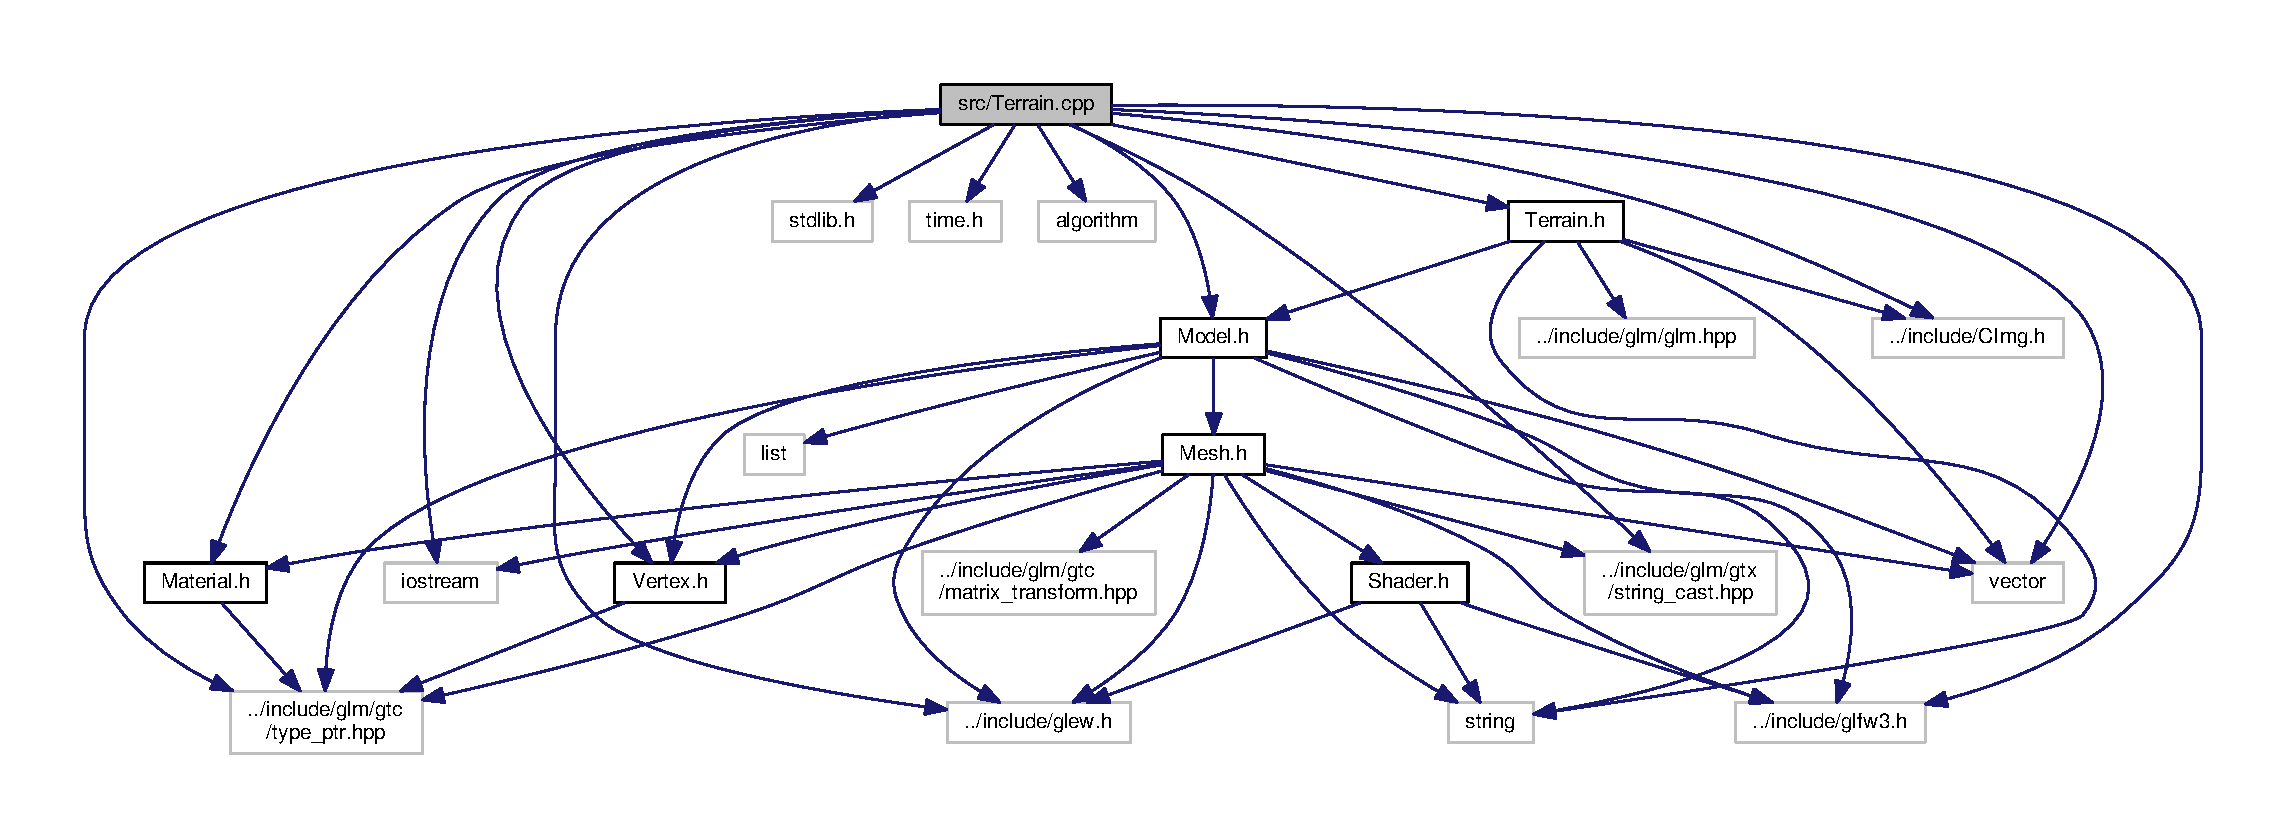
\includegraphics[width=350pt]{_terrain_8cpp__incl}
\end{center}
\end{figure}

\hypertarget{_terrain_8h}{}\section{src/\+Terrain.h File Reference}
\label{_terrain_8h}\index{src/\+Terrain.\+h@{src/\+Terrain.\+h}}
{\ttfamily \#include $<$string$>$}\\*
{\ttfamily \#include $<$vector$>$}\\*
{\ttfamily \#include \char`\"{}../include/\+C\+Img.\+h\char`\"{}}\\*
{\ttfamily \#include \char`\"{}../include/glm/glm.\+hpp\char`\"{}}\\*
{\ttfamily \#include \char`\"{}Model.\+h\char`\"{}}\\*
Include dependency graph for Terrain.\+h\+:\nopagebreak
\begin{figure}[H]
\begin{center}
\leavevmode
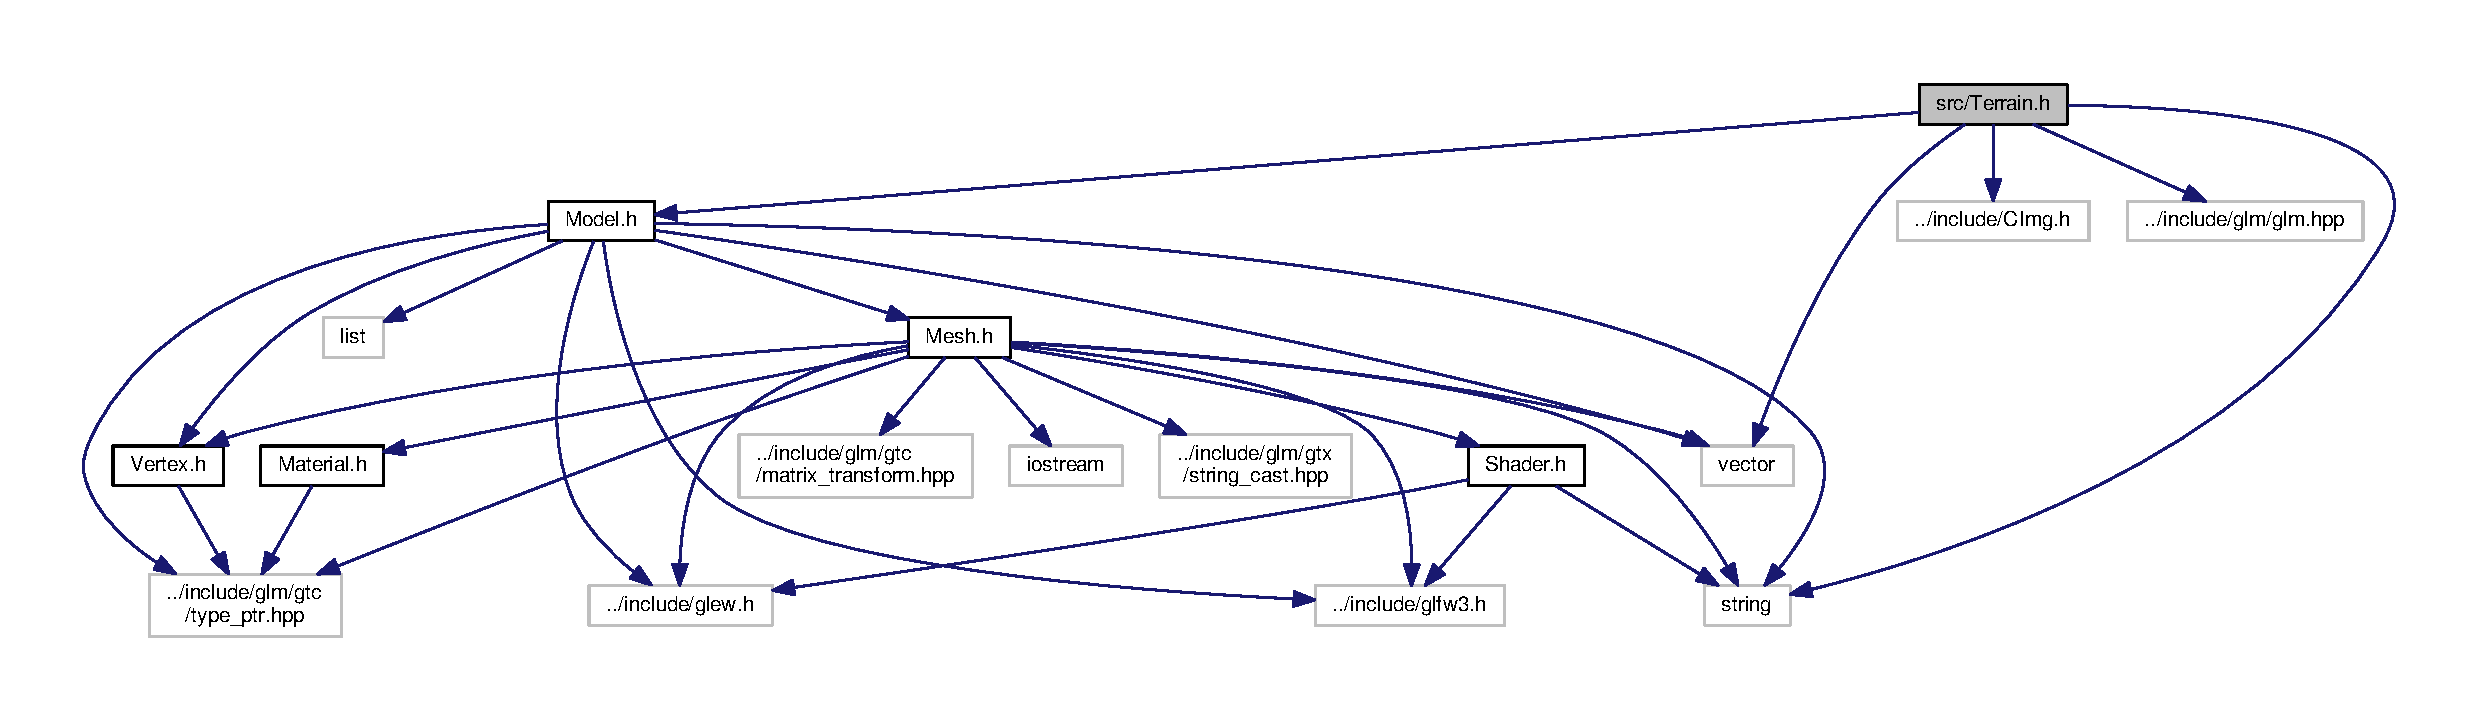
\includegraphics[width=350pt]{_terrain_8h__incl}
\end{center}
\end{figure}
This graph shows which files directly or indirectly include this file\+:\nopagebreak
\begin{figure}[H]
\begin{center}
\leavevmode
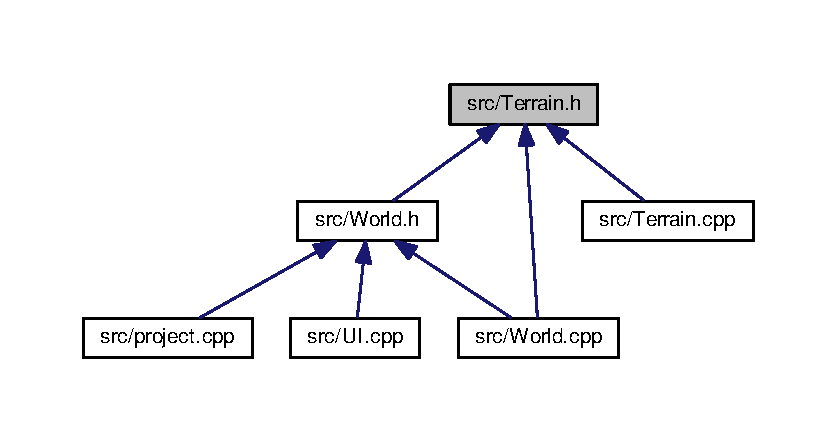
\includegraphics[width=350pt]{_terrain_8h__dep__incl}
\end{center}
\end{figure}
\subsection*{Classes}
\begin{DoxyCompactItemize}
\item 
class \hyperlink{class_terrain}{Terrain}
\end{DoxyCompactItemize}

\hypertarget{_tree_8cpp}{}\section{src/\+Tree.cpp File Reference}
\label{_tree_8cpp}\index{src/\+Tree.\+cpp@{src/\+Tree.\+cpp}}
{\ttfamily \#include \char`\"{}Tree.\+h\char`\"{}}\\*
{\ttfamily \#include $<$vector$>$}\\*
{\ttfamily \#include $<$stdio.\+h$>$}\\*
{\ttfamily \#include $<$iostream$>$}\\*
{\ttfamily \#include $<$string$>$}\\*
{\ttfamily \#include $<$cstring$>$}\\*
{\ttfamily \#include $<$algorithm$>$}\\*
{\ttfamily \#include \char`\"{}../include/glm/gtc/type\+\_\+ptr.\+hpp\char`\"{}}\\*
{\ttfamily \#include \char`\"{}Vertex.\+h\char`\"{}}\\*
{\ttfamily \#include \char`\"{}Mesh.\+h\char`\"{}}\\*
{\ttfamily \#include \char`\"{}Shader.\+h\char`\"{}}\\*
{\ttfamily \#include \char`\"{}Material.\+h\char`\"{}}\\*
{\ttfamily \#include \char`\"{}L\+System.\+h\char`\"{}}\\*
{\ttfamily \#include \char`\"{}Turtle.\+h\char`\"{}}\\*
Include dependency graph for Tree.\+cpp\+:\nopagebreak
\begin{figure}[H]
\begin{center}
\leavevmode
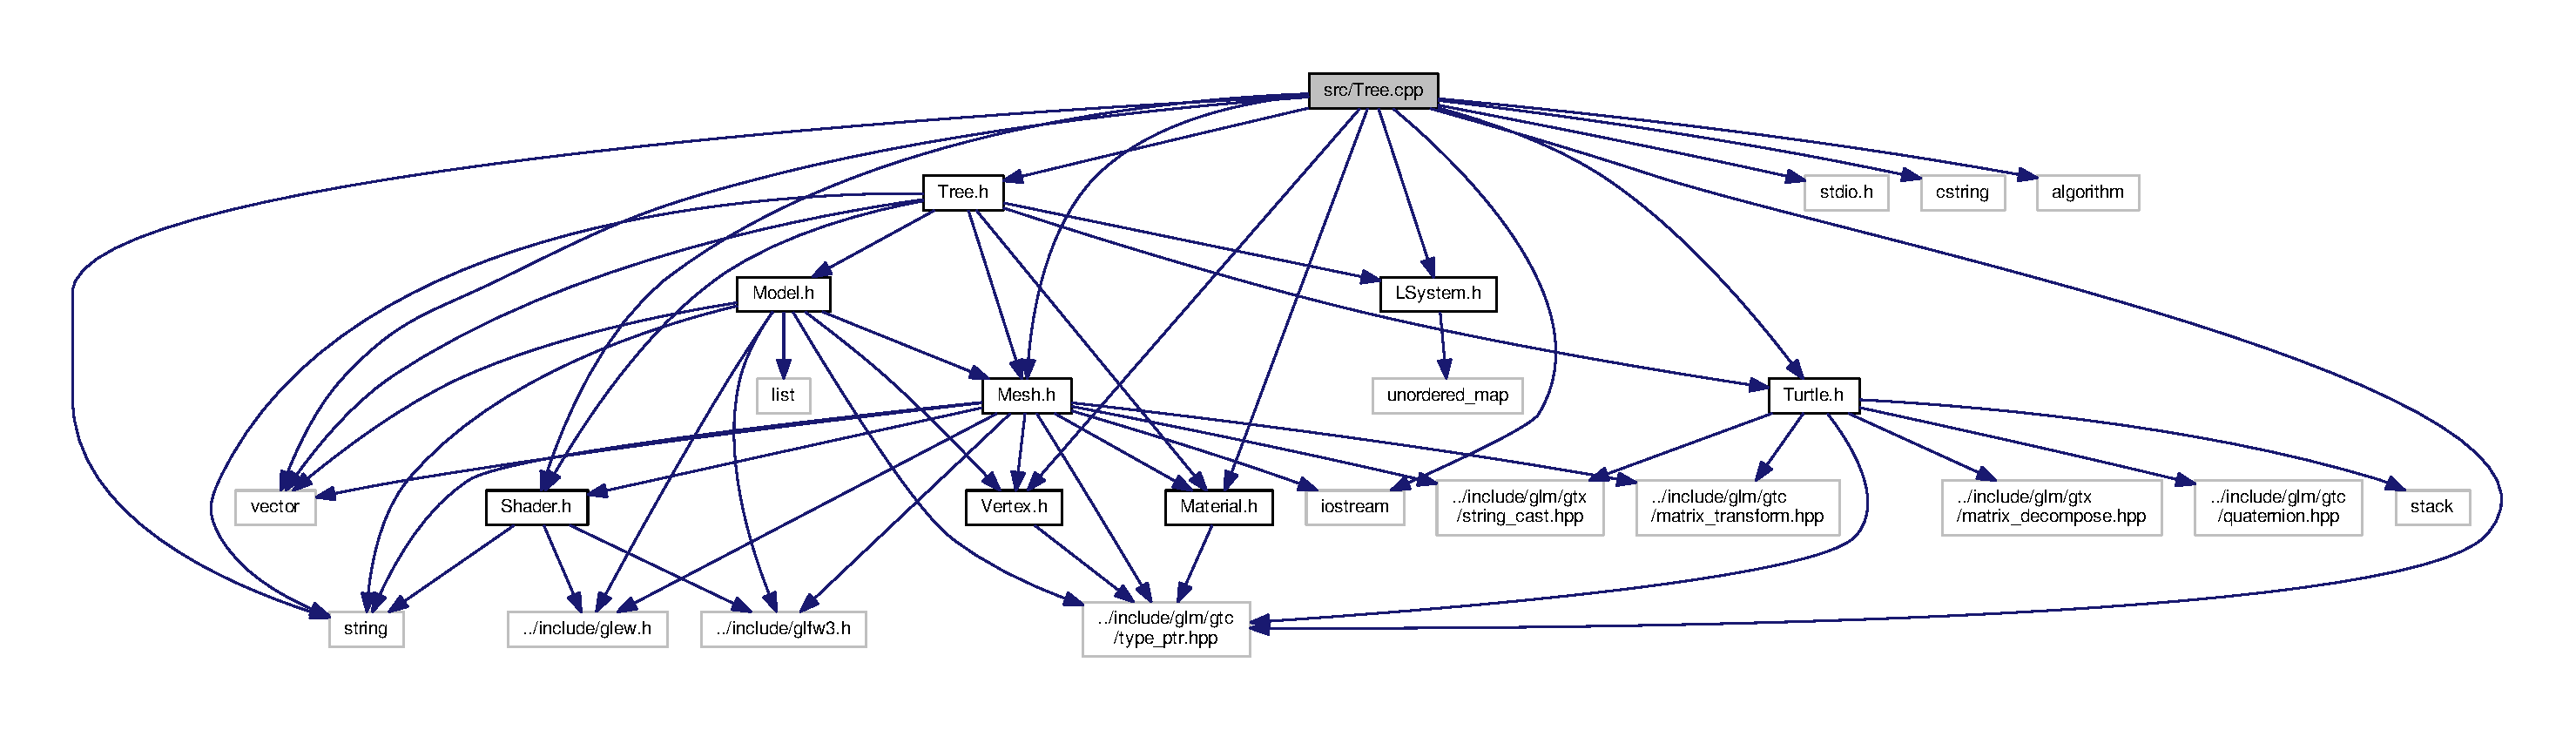
\includegraphics[width=350pt]{_tree_8cpp__incl}
\end{center}
\end{figure}

\hypertarget{_tree_8h}{}\section{src/\+Tree.h File Reference}
\label{_tree_8h}\index{src/\+Tree.\+h@{src/\+Tree.\+h}}
{\ttfamily \#include $<$vector$>$}\\*
{\ttfamily \#include $<$string$>$}\\*
{\ttfamily \#include \char`\"{}Shader.\+h\char`\"{}}\\*
{\ttfamily \#include \char`\"{}Material.\+h\char`\"{}}\\*
{\ttfamily \#include \char`\"{}Mesh.\+h\char`\"{}}\\*
{\ttfamily \#include \char`\"{}Model.\+h\char`\"{}}\\*
{\ttfamily \#include \char`\"{}L\+System.\+h\char`\"{}}\\*
{\ttfamily \#include \char`\"{}Turtle.\+h\char`\"{}}\\*
Include dependency graph for Tree.\+h\+:\nopagebreak
\begin{figure}[H]
\begin{center}
\leavevmode
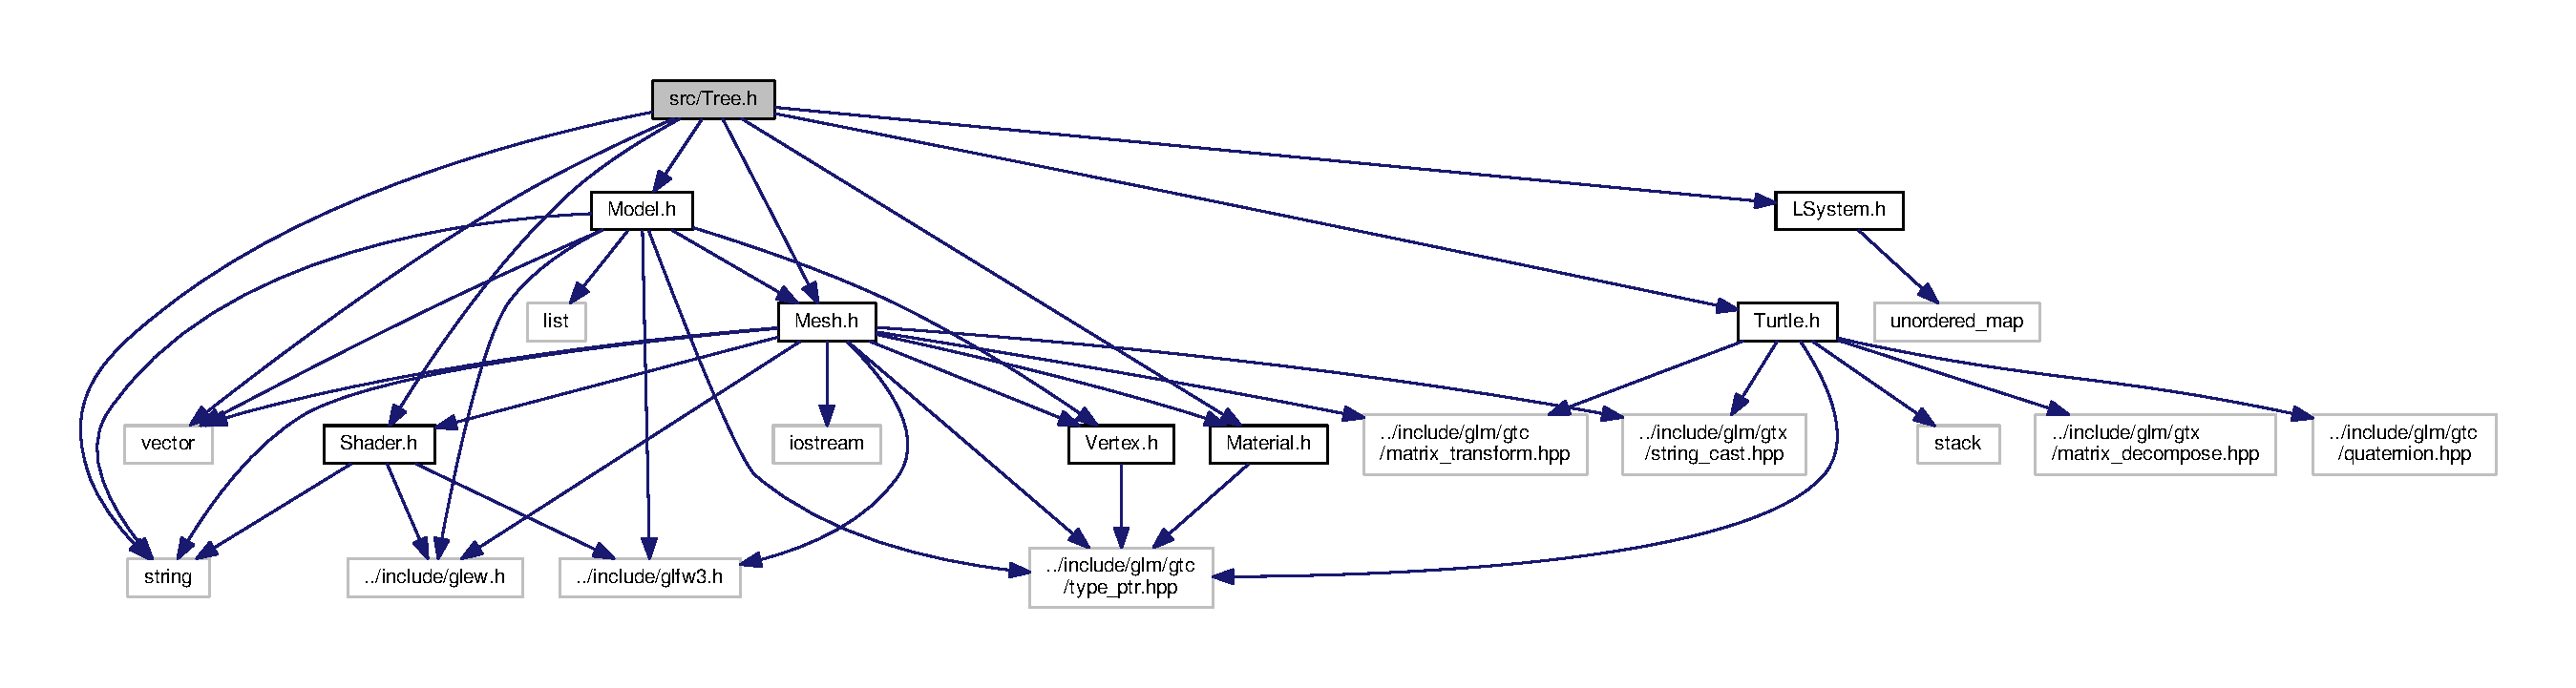
\includegraphics[width=350pt]{_tree_8h__incl}
\end{center}
\end{figure}
This graph shows which files directly or indirectly include this file\+:\nopagebreak
\begin{figure}[H]
\begin{center}
\leavevmode
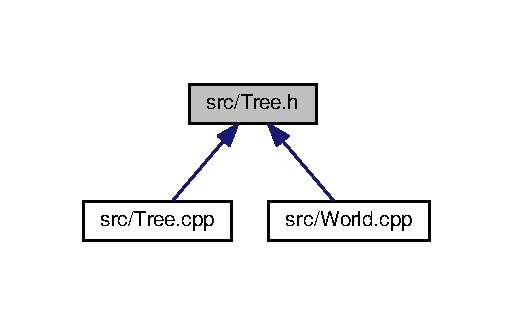
\includegraphics[width=246pt]{_tree_8h__dep__incl}
\end{center}
\end{figure}
\subsection*{Classes}
\begin{DoxyCompactItemize}
\item 
class \hyperlink{class_tree}{Tree}
\item 
struct \hyperlink{struct_tree_1_1lsys_data}{Tree\+::lsys\+Data}
\end{DoxyCompactItemize}

\hypertarget{_turtle_8h}{}\section{src/\+Turtle.h File Reference}
\label{_turtle_8h}\index{src/\+Turtle.\+h@{src/\+Turtle.\+h}}
{\ttfamily \#include $<$stack$>$}\\*
{\ttfamily \#include \char`\"{}../include/glm/gtc/type\+\_\+ptr.\+hpp\char`\"{}}\\*
{\ttfamily \#include \char`\"{}../include/glm/gtc/matrix\+\_\+transform.\+hpp\char`\"{}}\\*
{\ttfamily \#include \char`\"{}../include/glm/gtx/matrix\+\_\+decompose.\+hpp\char`\"{}}\\*
{\ttfamily \#include \char`\"{}../include/glm/gtc/quaternion.\+hpp\char`\"{}}\\*
{\ttfamily \#include \char`\"{}../include/glm/gtx/string\+\_\+cast.\+hpp\char`\"{}}\\*
Include dependency graph for Turtle.\+h\+:\nopagebreak
\begin{figure}[H]
\begin{center}
\leavevmode
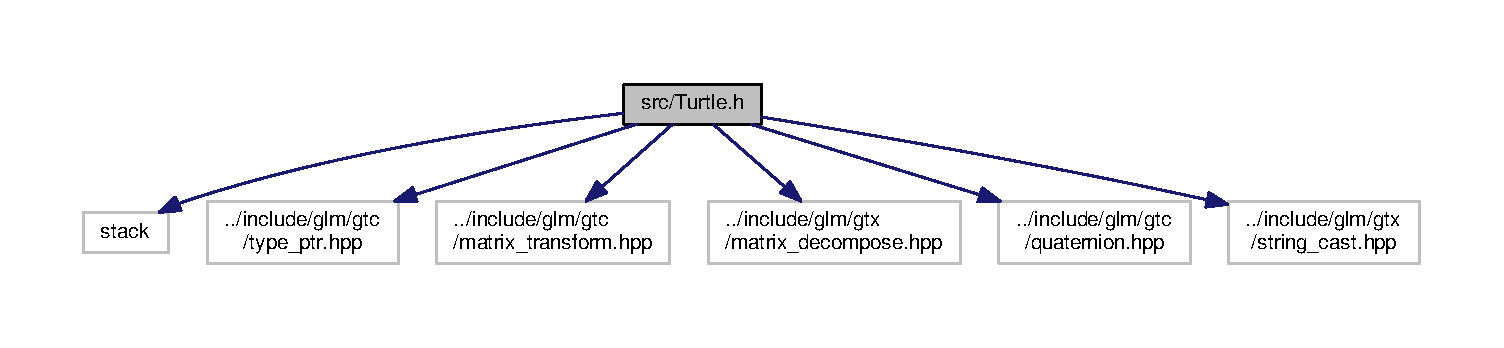
\includegraphics[width=350pt]{_turtle_8h__incl}
\end{center}
\end{figure}
This graph shows which files directly or indirectly include this file\+:\nopagebreak
\begin{figure}[H]
\begin{center}
\leavevmode
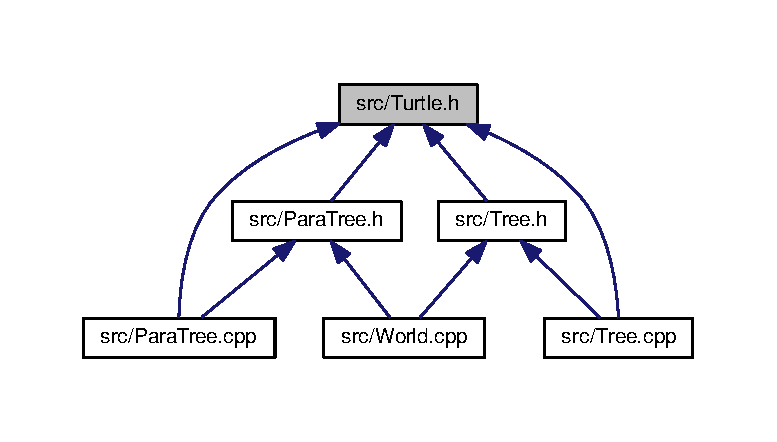
\includegraphics[width=350pt]{_turtle_8h__dep__incl}
\end{center}
\end{figure}
\subsection*{Classes}
\begin{DoxyCompactItemize}
\item 
class \hyperlink{class_turtle}{Turtle}
\item 
struct \hyperlink{struct_turtle_1_1_transformation_set}{Turtle\+::\+Transformation\+Set}
\end{DoxyCompactItemize}

\hypertarget{_u_i_8cpp}{}\section{src/\+UI.cpp File Reference}
\label{_u_i_8cpp}\index{src/\+U\+I.\+cpp@{src/\+U\+I.\+cpp}}
{\ttfamily \#include \char`\"{}../include/glew.\+h\char`\"{}}\\*
{\ttfamily \#include \char`\"{}../include/glfw3.\+h\char`\"{}}\\*
{\ttfamily \#include \char`\"{}U\+I.\+h\char`\"{}}\\*
{\ttfamily \#include \char`\"{}World.\+h\char`\"{}}\\*
{\ttfamily \#include \char`\"{}Camera.\+h\char`\"{}}\\*
Include dependency graph for U\+I.\+cpp\+:\nopagebreak
\begin{figure}[H]
\begin{center}
\leavevmode
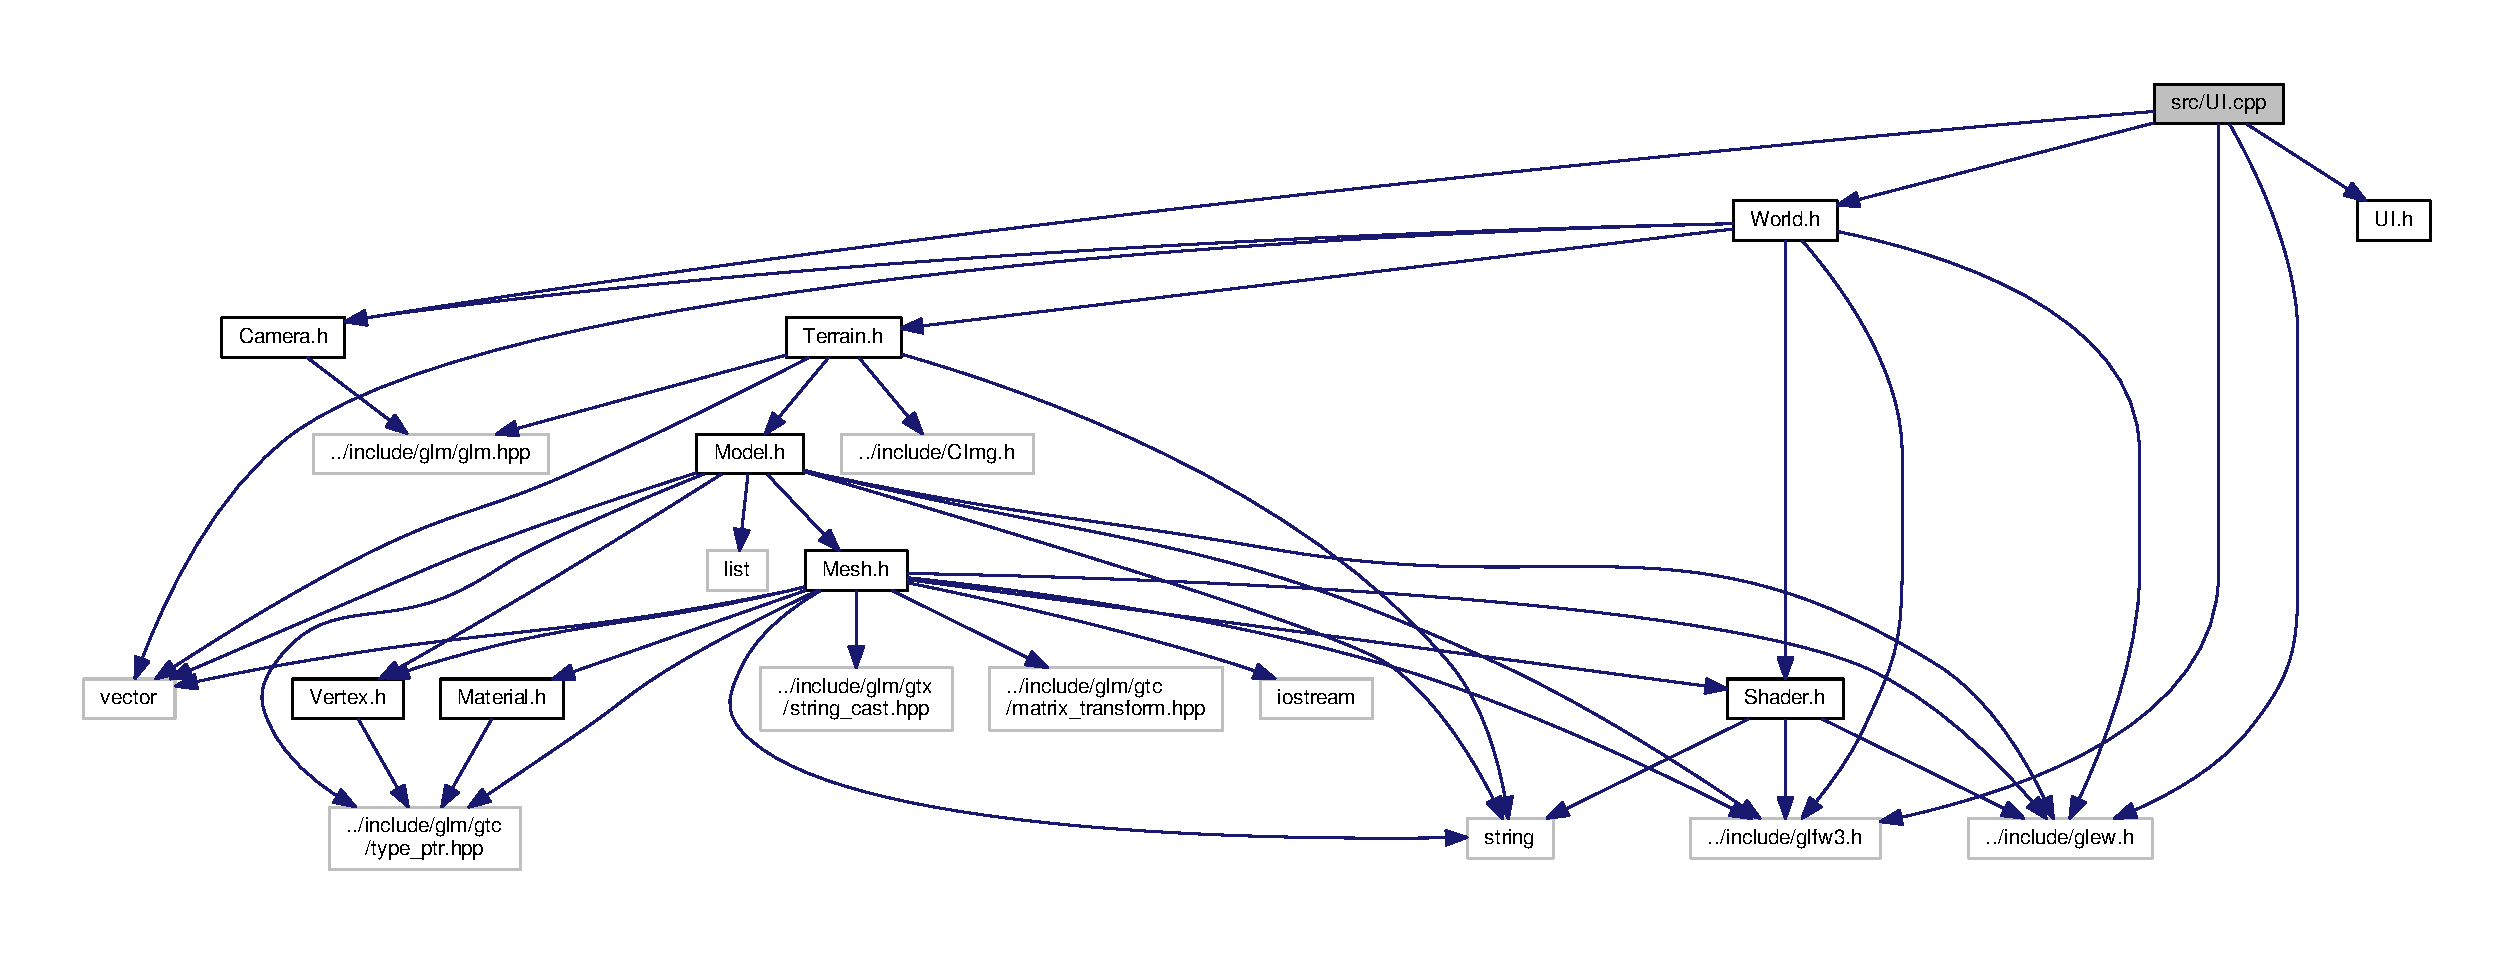
\includegraphics[width=350pt]{_u_i_8cpp__incl}
\end{center}
\end{figure}
\subsection*{Namespaces}
\begin{DoxyCompactItemize}
\item 
 \hyperlink{namespace_u_i}{UI}
\end{DoxyCompactItemize}
\subsection*{Functions}
\begin{DoxyCompactItemize}
\item 
void \hyperlink{namespace_u_i_a16e5aee40bc2d40e67afdfe6749ecc12}{U\+I\+::init} (\hyperlink{class_world}{World} $\ast$world, G\+L\+F\+Wwindow $\ast$window)
\item 
void \hyperlink{namespace_u_i_af31deeef2d9fe94fa317bdf1adc6e942}{U\+I\+::set\+Active} (U\+I\+Base \&U\+Iinstance)
\end{DoxyCompactItemize}
\subsection*{Variables}
\begin{DoxyCompactItemize}
\item 
const float \hyperlink{namespace_u_i_a3acb427a17b83fb6a34d117989a7c435}{U\+I\+::\+M\+O\+U\+S\+E\+\_\+\+S\+E\+N\+S\+\_\+\+M\+OV} = 0.\+05f
\item 
const float \hyperlink{namespace_u_i_a807544150b32fe6af7851672f882500b}{U\+I\+::\+C\+A\+M\+E\+R\+A\+\_\+\+F\+OV} = 45.\+0f
\item 
\hyperlink{class_world}{World} $\ast$ \hyperlink{namespace_u_i_a84dc8a978d6b785608801d14bac894b7}{U\+I\+::world}
\item 
G\+L\+F\+Wwindow $\ast$ \hyperlink{namespace_u_i_ac05ba8c1833c723ee85c762399654d3e}{U\+I\+::window}
\item 
U\+I\+Explore \hyperlink{namespace_u_i_a5724793eec5b84e087210957c562dad6}{U\+I\+::\+Explore}
\end{DoxyCompactItemize}

\hypertarget{_u_i_8h}{}\section{src/\+UI.h File Reference}
\label{_u_i_8h}\index{src/\+U\+I.\+h@{src/\+U\+I.\+h}}
This graph shows which files directly or indirectly include this file\+:\nopagebreak
\begin{figure}[H]
\begin{center}
\leavevmode
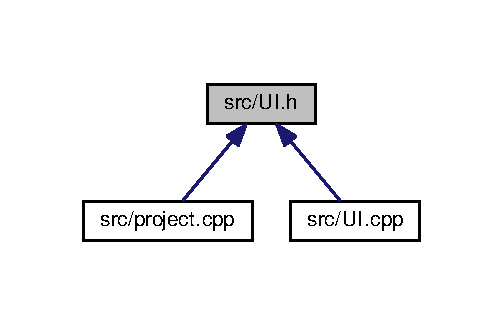
\includegraphics[width=242pt]{_u_i_8h__dep__incl}
\end{center}
\end{figure}
\subsection*{Classes}
\begin{DoxyCompactItemize}
\item 
class \hyperlink{class_u_i_1_1_u_i_base}{U\+I\+::\+U\+I\+Base}
\item 
class \hyperlink{class_u_i_1_1_u_i_explore}{U\+I\+::\+U\+I\+Explore}
\end{DoxyCompactItemize}
\subsection*{Namespaces}
\begin{DoxyCompactItemize}
\item 
 \hyperlink{namespace_u_i}{UI}
\end{DoxyCompactItemize}
\subsection*{Functions}
\begin{DoxyCompactItemize}
\item 
void \hyperlink{namespace_u_i_a16e5aee40bc2d40e67afdfe6749ecc12}{U\+I\+::init} (\hyperlink{class_world}{World} $\ast$world, G\+L\+F\+Wwindow $\ast$window)
\item 
void \hyperlink{namespace_u_i_af31deeef2d9fe94fa317bdf1adc6e942}{U\+I\+::set\+Active} (U\+I\+Base \&U\+Iinstance)
\end{DoxyCompactItemize}

\hypertarget{_vertex_8h}{}\section{src/\+Vertex.h File Reference}
\label{_vertex_8h}\index{src/\+Vertex.\+h@{src/\+Vertex.\+h}}
{\ttfamily \#include \char`\"{}../include/glm/gtc/type\+\_\+ptr.\+hpp\char`\"{}}\\*
Include dependency graph for Vertex.\+h\+:\nopagebreak
\begin{figure}[H]
\begin{center}
\leavevmode
\includegraphics[width=172pt]{_vertex_8h__incl}
\end{center}
\end{figure}
This graph shows which files directly or indirectly include this file\+:
\nopagebreak
\begin{figure}[H]
\begin{center}
\leavevmode
\includegraphics[width=350pt]{_vertex_8h__dep__incl}
\end{center}
\end{figure}
\subsection*{Classes}
\begin{DoxyCompactItemize}
\item 
struct \hyperlink{struct_vertex}{Vertex}
\end{DoxyCompactItemize}

\hypertarget{_world_8cpp}{}\section{src/\+World.cpp File Reference}
\label{_world_8cpp}\index{src/\+World.\+cpp@{src/\+World.\+cpp}}
{\ttfamily \#include $<$string$>$}\\*
{\ttfamily \#include $<$vector$>$}\\*
{\ttfamily \#include \char`\"{}../include/glew.\+h\char`\"{}}\\*
{\ttfamily \#include \char`\"{}../include/glfw3.\+h\char`\"{}}\\*
{\ttfamily \#include \char`\"{}../include/glm/gtc/type\+\_\+ptr.\+hpp\char`\"{}}\\*
{\ttfamily \#include \char`\"{}Shader.\+h\char`\"{}}\\*
{\ttfamily \#include \char`\"{}Terrain.\+h\char`\"{}}\\*
{\ttfamily \#include \char`\"{}Camera.\+h\char`\"{}}\\*
{\ttfamily \#include \char`\"{}Material.\+h\char`\"{}}\\*
{\ttfamily \#include \char`\"{}Model.\+h\char`\"{}}\\*
{\ttfamily \#include \char`\"{}Tree.\+h\char`\"{}}\\*
{\ttfamily \#include \char`\"{}Para\+Tree.\+h\char`\"{}}\\*
{\ttfamily \#include \char`\"{}World.\+h\char`\"{}}\\*
{\ttfamily \#include $<$iostream$>$}\\*
{\ttfamily \#include \char`\"{}../include/glm/gtx/string\+\_\+cast.\+hpp\char`\"{}}\\*
Include dependency graph for World.\+cpp\+:\nopagebreak
\begin{figure}[H]
\begin{center}
\leavevmode
\includegraphics[width=350pt]{_world_8cpp__incl}
\end{center}
\end{figure}

\hypertarget{_world_8h}{}\section{src/\+World.h File Reference}
\label{_world_8h}\index{src/\+World.\+h@{src/\+World.\+h}}
{\ttfamily \#include $<$vector$>$}\\*
{\ttfamily \#include \char`\"{}../include/glew.\+h\char`\"{}}\\*
{\ttfamily \#include \char`\"{}../include/glfw3.\+h\char`\"{}}\\*
{\ttfamily \#include \char`\"{}Shader.\+h\char`\"{}}\\*
{\ttfamily \#include \char`\"{}Terrain.\+h\char`\"{}}\\*
{\ttfamily \#include \char`\"{}Camera.\+h\char`\"{}}\\*
Include dependency graph for World.\+h\+:\nopagebreak
\begin{figure}[H]
\begin{center}
\leavevmode
\includegraphics[width=350pt]{_world_8h__incl}
\end{center}
\end{figure}
This graph shows which files directly or indirectly include this file\+:\nopagebreak
\begin{figure}[H]
\begin{center}
\leavevmode
\includegraphics[width=337pt]{_world_8h__dep__incl}
\end{center}
\end{figure}
\subsection*{Classes}
\begin{DoxyCompactItemize}
\item 
class \hyperlink{class_world}{World}
\end{DoxyCompactItemize}

%--- End generated contents ---

% Index
\backmatter
\newpage
\phantomsection
\clearemptydoublepage
\addcontentsline{toc}{chapter}{Index}
\printindex

\end{document}
